% !TeX spellcheck = en_GB
%% ----------------------------------------------------------------
%% Thesis.tex -- MAIN FILE (the one that you compile with LaTeX)
%% ---------------------------------------------------------------- 

% Set up the document
\pdfminorversion=4
\documentclass[a4paper, 11pt, twoside, oneside]{Thesis}  % Use the "Thesis" style, based on the ECS Thesis style by Steve Gunn


% Bella used 18pt Times New Roman with Double Spacing.

% SETUP

% TikZ stuff
\usetikzlibrary{shapes, graphs, quotes, arrows, backgrounds, positioning, calc}
\usepackage{dot2texi}

% Glossaries
\setacronymstyle{long-short}  

%http://tex.stackexchange.com/questions/89166/centering-in-tabularx-and-x-columns
\newcolumntype{Y}{>{\centering\arraybackslash}X}

% Graphics
\DeclareGraphicsExtensions{.pdf,.jpg,.png}
\graphicspath{{./Figures/}{./Figures/img/}{../../Dropbox/Thesis_Figures/}}  % Location of the graphics files (set up for graphics to be in PDF format)
\presetkeys%
    {todonotes}%
    {inline,backgroundcolor=yellow}{}


% Network terms

\newacronym{manet}{MANET}{Mobile Ad-hoc Network}  
\newacronym{otmf}{OTMF}{Objective Trust Management Framework}
\newacronym{plr}{PLR}{Packet Loss Rate}
\newacronym{tmf}{TMF}{Trust Management Framework}
\newacronym{mtfm}{MTFM}{Multi-parameter Trust Framework for MANETs}
\newacronym{v2v}{V2V}{Vehicle to Vehicle}
\newacronym{ttp}{TTP}{Trusted Third Party}
\newacronym{pki}{PKI}{Public Key Infrastructure}
\newacronym{mac}{MAC}{Medium Access Control}
\newacronym{rts}{RTS}{Request To Send}

% Routing Stuff
\newacronym{ospf}{OSPF}{Open Shortest Path First}
%% Proactive
\newacronym{cgsr}{CGSR}{Cluster-head Gateway Switch Routing}
\newacronym{dream}{DREAM}{Distance Routing Effect Algorithm for Mobility}
\newacronym{dsdv}{DSDV}{Destination-Sequences Distance Vector}
\newacronym{fsr}{FSR}{Fisheye State Routing}
\newacronym{gsr}{GSR}{Global State Routing}
\newacronym{hsr}{HSR}{Hierarchial State Routing}
\newacronym{mmwn}{MMWN}{Multimedia support in Mobile Wireless Networks}
\newacronym{olsr}{OLSR}{Optimised Link State Routing}
\newacronym{star}{STAR}{Source Tree Adaptive Routing}
\newacronym{tbrpf}{TBRPF}{Topology Dissemination Based On Reverse-Path Forwarding}
\newacronym{wrp}{WRP}{Wireless Routing Protocol}
%% Reactive 
\newacronym{dsr}{DSR}{Dynamic Source Routing}
\newacronym{aodv}{AODV}{Ad hoc On-demand Distance Vector}
\newacronym{roam}{ROAM}{Routing On-demand Acyclic Multipath}
\newacronym{abr}{ABR}{Associativity Based Routing}
\newacronym{lar}{LAR}{Location Aided Routing}
\newacronym{cbrp}{CBRP}{Cluster Based Routing Protocol}
%% Hybrid
\newacronym{zrp}{ZRP}{Zone Routing Protocol}
\newacronym{dst}{DST}{Distributed Spanning Trees}
\newacronym{ddr}{DDR}{Distributed Dynamic Routing}
\newacronym{zhls}{ZHLS}{Zone-based Hierarchial Link State}
\newacronym{slurp}{SLURP}{Scalable Location Update Routing Protocol}

% Mil Terms
\newacronym{mcm}{MCM}{Mine-Counter Measure}
\newacronym{mhc}{MHC}{Maritime Hydrography Capability}
\newacronym{eod}{EOD}{Explosive Ordnance Disposal}
\newacronym{los}{LOS}{Line of Sight}
\newacronym{blos}{BLOS}{Beyond Line of Sight}
\newacronym{isr}{ISR}{Intelligence, Surveillance and Reconnaissance}
\newacronym{cmre}{CMRE}{Centre for Maritime Research and Experimentation}
\newacronym{dstl}{DSTL}{Defence Science and Technology Laboratory}
\newacronym{sae}{SAE}{Society of Automotive Engineers}
\newacronym{astm}{ASTM}{American Society of Testing and Materials}
\newacronym{vsm}{VSM}{Vehicle Specific Module}
\newacronym{dli}{DLI}{Data Link Interface}
\newacronym{stanag}{STANAG}{NATO Standardization Agreement}

% Hardware Terms
\newacronym{auv}{AUV}{Autonomous Underwater Vehicle}
\newacronym{uav}{UAV}{Unmanned Aerial Vehicle}
\newacronym{umvs}{UMVS}{Unmanned Maritime Vehicle System}
\newacronym{uan}{UAN}{Underwater Acoustic Network}
\newacronym{gps}{GPS}{Global Positioning System}


% Autonomy Terms
\newacronym{loa}{LOA}{Level of Automation}
\newacronym{loi}{LOI}{Level of Interoperabilty}
\newacronym{hsc}{HSC}{Human Supervisory Control}
\newacronym{jaus}{JAUS}{Joint Architecture for Unmanned Systems}
\newacronym{hri}{HRI}{Human Robot Interaction}
\newacronym{sos}{SoS}{System of Systems}

% Math
\newacronym{grc}{GRC}{Grey Relational Coefficient}


% MY Terms
\newacronym{indd}{INDD}{Inter-Node Distance Deviation}
\newacronym{inhd}{INHD}{Inter-Node Heading Deviation}
\newacronym{acs}{ACS}{Autonomous Collaborative System}
\newacronym{mpc}{MPC}{Malicious Power Control}
\newacronym{sts}{STS}{Selfish Target Selection}
 % Glossaries Definitions
\makeglossaries


% Include any extra LaTeX packages required

%% ----------------------------------------------------------------
\begin{document}
%http://tex.stackexchange.com/questions/32867/tikz-rectangular-node-with-different-rounded-corners
\makeatletter
\pgfdeclareshape{roundedNode}{
	\inheritsavedanchors[from=rectangle] % this is nearly a rectangle
	\inheritanchorborder[from=rectangle]
	\inheritanchor[from=rectangle]{center}
	\inheritanchor[from=rectangle]{north}
	\inheritanchor[from=rectangle]{south}
	\inheritanchor[from=rectangle]{west}
	\inheritanchor[from=rectangle]{east}
	\backgroundpath{% this is new
		% store lower right in xa/ya and upper right in xb/yb
		\southwest \pgf@xa=\pgf@x \pgf@ya=\pgf@y
		\northeast \pgf@xb=\pgf@x \pgf@yb=\pgf@y
		% construct main path
		\pgfsetcornersarced{\pgfpoint{5pt}{5pt}}
		\pgfpathmoveto{\pgfpoint{\pgf@xa}{\pgf@ya}}
		\pgfpathlineto{\pgfpoint{\pgf@xa}{\pgf@yb}}
		\pgfpathlineto{\pgfpoint{\pgf@xb}{\pgf@yb}}
		\pgfsetcornersarced{\pgfpoint{5pt}{5pt}}
		\pgfpathlineto{\pgfpoint{\pgf@xb}{\pgf@ya}}
		\pgfpathclose
	}
}
% http://tex.stackexchange.com/questions/98388/how-to-make-table-with-rotated-table-headers-in-latex
\newcommand*\rot{\rotatebox{90}}
\newcommand*\OK{\ding{51}} % requires pifont

\makeatother
%http://tex.stackexchange.com/questions/132783/how-to-write-checkmark-in-latex
\def\checkmark{\tikz\fill[scale=0.4](0,.35) -- (.25,0) -- (1,.7) -- (.25,.15) -- cycle;} 

\tikzset{
	block/.style = {draw, fill=white, rectangle, minimum height=3em, minimum width=3em, text width=8em, text centered},
	tmp/.style  = {coordinate}, 
	sum/.style= {draw, fill=white, circle, node distance=1cm},
	input/.style = {coordinate},
	output/.style= {coordinate},
	pinstyle/.style = {pin edge={to-,thin,black}
	},
	from/.style args={#1 to #2}{% without transformations
		above right={0cm of #1},% needs positioning library
		/utils/exec=\pgfpointdiff
		{\tikz@scan@one@point\pgfutil@firstofone(#1)\relax}
		{\tikz@scan@one@point\pgfutil@firstofone(#2)\relax},
		minimum width/.expanded=\the\pgf@x,
		minimum height/.expanded=\the\pgf@y},
	doc/.style={draw, shape=roundedNode, align=center},
	bluefill/.style={fill=blue, opacity=0.5, text opacity=1}
}
\tikzset{
	*|/.style={
		to path={
			(perpendicular cs: horizontal line through={(\tikztostart)},
			vertical line through={(\tikztotarget)})
			% is the same as (\tikztostart -| \tikztotarget)
			% but just to be safe: http://tex.stackexchange.com/a/29781/16595
			-- (\tikztotarget) \tikztonodes
		}
	}
}

% USAGE: \cercle {center} {radius in cm} {begin degrees} {value of the arc} {line width} {color}
% \coordinate (OO) at (2.8,2.2);
% \cercle{OO}{0.5cm}{-20}{60}{1.0pt}{blue};
\newcommand{\cercle}[6]{
\node[circle,inner sep=0,minimum size={2*#2}](a) at (#1) {};
\draw[#6,line width=#5] (a.#3) arc (#3:{#3+#4}:#2);
}


% \SpecialCoor
\def\subsum{\mathit{\Sigma}}

\setcounter{secnumdepth}{2}
\setcounter{tocdepth}{2}


\newenvironment{myindentpar}[1]%
{\begin{list}{}%
         {\setlength{\leftmargin}{#1}}%
         \item[]%
}
{\end{list}}


\renewcommand*{\figureautorefname}{Fig.}
\renewcommand*{\chapterautorefname}{Chapter}
\renewcommand*{\sectionautorefname}{Section}
\renewcommand*{\subsectionautorefname}{Subsection}

\newcommand*{\fullref}[1]{\hyperref[{#1}]{\autoref*{#1} \nameref*{#1}}} % One single link

 % Introduction
\pagestyle{plain}  % Return the page headers back to the "fancy" style
\frontmatter	  % Begin Roman style (i, ii, iii, iv...) page numbering


\maketitle
%% ----------------------------------------------------------------


\setstretch{1}  % It is better to have smaller font and larger line spacing than the other way round

% Define the page headers using the FancyHdr package and set up for one-sided printing
\fancyhead{}  % Clears all page headers and footers
\rhead{\thepage}  % Sets the right side header to show the page number
\lhead{}  % Clears the left side page header

\cleardoublepage  % Declaration ended, now start a new page

\onehalfspacing
{\hypersetup{linkcolor=black}
\tableofcontents  % Write out the Table of Contents
 \clearpage      

\listoffigures  % Write out the List of Figures

\listoftables  % Write out the List of Tables
}

\cleardoublepage  %Start a new page

%\listofnomenclature{lll}  % Include a list of Symbols (a three column table)
\glsaddall
\printglossaries
\glsresetall


\cleardoublepage  
\addtotoc{Preface}  
\addtocontents{toc}{\vspace{1em}}  % Add a gap in the Contents, for aesthetics
\chapter*{Preface}
This thesis is primarily my own work. The sources of other materials are identifed.



\cleardoublepage  
\addtotoc{Abstract}  % Add the "Abstract" page entry to the Contents
\addtocontents{toc}{\vspace{1em}}  % Add a gap in the Contents, for aesthetics
\chapter*{Abstract}
As \glspl{auv} become more technically capable and economically feasible, they are being increasingly used in a great many areas of defence, commercial and environmental applications. 
These applications are tending towards using independent, autonomous, ad-hoc, collaborative behaviour of teams or fleets of these \gls{auv} platforms.
This convergence of research experiences in the \gls{uan} and \gls{manet} fields, along with the increasing \gls{loa} of such platforms, creates unique challenges to secure the operation and communication of these networks.

The question of security and reliability of operation in networked systems has usually been resolved by having a centralised coordinating agent to manage shared secrets and monitor for misbehaviour.
However, in the sparse, noisy and constrained communications environment of \glspl{uan}, the communications overheads and single-point-of-failure risk of this model is challenged (particularly when faced with capable attackers).

As such, more lightweight, distributed, experience based\footnote{rather than ``Evidence based'' in the case of shared keys, \gls{pki} etc.} systems of ``Trust'' have been proposed to dynamically model and evaluate the ``trustworthiness'' of nodes within a \gls{manet} across the network to prevent or isolate the impact of malicious, selfish, or faulty misbehaviour. 
Previously, these models have monitored actions purely within the communications domain. 
Moreover, the vast majority rely on only one type of observation (metric) to evaluate trust; successful packet forwarding.
In these cases, motivated actors may use this limited scope of observation to either perform unfairly without repercussions in other domains/metrics, or to make another, fair, node appear to be operating unfairly.

This thesis is primarily concerned with the use of terrestrial-\gls{manet} trust frameworks to the \gls{uan} space. 
Considering the massive theoretical and practical difference in the communications environment, these frameworks must be reassessed for suitability to the marine realm. 
We find that current single-metric \glspl{tmf} do not perform well in a best-case scaling of the marine network, due to sparse and noisy observation metrics, and while basic multi-metric communications-only frameworks perform better than their single-metric forms, this performance is still not at a reliable level. 
We propose, demonstrate (through simulation) and integrate the use of physical observational metrics for trust assessment, in tandem with metrics from the communications realm, improving the safety, security, reliability and integrity of autonomous \glspl{uan}.

Three main novelties are demonstrated in this work:
Trust evaluation using metrics from the physical domain (movement/distribution/etc.), demonstration of the failings of Communications-based Trust evaluation in sparse, noisy, delayful and non-linear \gls{uan} environments, and the deployment of trust assessment across multiple domains, e.g.\ the physical and communications domains.
The latter contribution includes the generation and optimisation of cross-domain metric composition or``synthetic domains'' as a performance improvement method.
 % Introduction
\cleardoublepage  % Declaration ended, now start a new page


\addtotoc{Acknowledgements}  % Add the "Abstract" page entry to the Contents
\addtocontents{toc}{\vspace{1em}}  % Add a gap in the Contents, for aesthetics
\chapter*{Acknowledgements}

There are many people who deserve the highest thanks for their support, patience, kindness and understanding.
The greatest thanks have to be distributed among my family and friends, for putting up with my madness; both the madness of starting it and the madness of seeing it through.
Maybe I'll get a job that you can actually explain! 
Finally, I must thank Professor Marshall, without whom this work wouldn't have been attempted let alone completed.

{\centering
Alan-hu Akbar\par
}
 % Introduction
\clearpage  % End of the Acknowledgements

\mainmatter	  % Begin normal, numeric (1,2,3...) page numbering
\pagestyle{fancy}  % Return the page headers back to the "fancy" style

% !TeX spellcheck = en_GB

\chapter{Introduction}
\label{ch:introduction}
\lhead{Chapter \thechapter. \emph{Introduction}}

\section{\glspl{manet}}\label{manets}

With the explosive growth in the use of mobile telephony and the increasing miniaturisation and efficiency gains of portable communications devices, the classical paradigm of a broadcast/receiver or server/client has given way to an increasing use of decentralised, ad-hoc networks that not only accommodate but take advantage of network mobility.

Whether these networks are decentralised cellular / RF / 802.11 WiFi networks for use in disaster relief areas \cite{Milliken2015} or biologically inspired wireless sensor networks for low-energy, low-maintenance environmental monitoring \cite{Nicholson2008,Selvakennedy2007}, \gls{manet} theory developed over the past 30 years has gone from it's first formal definition, emerging from DARPA's Packet Radio Network research \cite{Jubin1987}, to being an integral part of modern practical communications.

Minimally, a \gls{manet} consists of of a collection of mobile physical entities (nodes) that communicate cooperatively to collect, distribute, disseminate, and collate data and/or influence across an area.
In most cases \gls{manet} nodes incorporate bi-directional transceivers to send and receive data, however this bi-directionality is not a requirement (for example in the area of Wireless Sensor Networks \cite{Akyildiz2002}).
\glspl{manet} may utilise omnidirectional, static, or steerable communications antennae, and a selection of protocols such as WiFi, Bluetooth, GSM, UMTS, Optical or Acoustics, and may incorporate a range of mobilities across nodes, from static devices, terrestrial and marine surface platforms, and aerial and underwater platforms.
A core characteristic of \glspl{manet} is the inclusion and integration of heterogeneous node collections, i.e where different nodes or groups of nodes in a network may have different capabilities in terms of propulsion, sensor apparatus, communications capability, etc.

\glspl{manet} may be totally independent with no external connections; include independent per-node communications backhauls (e.g. Cellular Modems in mobile phones as part of a Bluetooth Personal Area Network), or include static nodes that provide infrastructure based backhaul.
However, this multiplicity of variations and options presents several challenges to users and operators; the physical topology of \glspl{manet} can vary wildly over short periods of time.
A particular challenge to \gls{manet} operation is that given any node may operate as a routing / gateway node, if/when that node moves to a different region, network segments that had previously used that node as a path must renegotiate / re-establish their routes.
These situations, if not appropriately managed, lead to opportunities for subversion and selfishness.

The characteristics of \gls{manet}s as defined by Corson et al.\ are paraphrased in Table~\ref{tab:manet_characteristics}.

\begin{table}[h!]
  \hyphenpenalty=10000
\caption[Summary of Characteristics of \glspl{manet}]{Summary of Characteristics of \glspl{manet}\cite{Corson1999}}
\label{tab:manet_characteristics}
  \begin{tabularx}{\textwidth}{p{2cm}X}\toprule
    Dynamic Topologies & Nodes are free to move arbitrarily; thus, the typically multi-hop network topology may change randomly and rapidly at unpredictable times, and may consist of both bidirectional and unidirectional links.
\\
    Bandwidth Constrained, Varied Capacity & Wireless links will continue to have significantly lower capacity than their hardwired counterparts.
In addition, the realized throughput of wireless communications, after accounting for the effects of multiple access, fading, noise, and interference conditions, etc., is often much less than a radio's maximum transmission rate.
\par
One effect of the relatively low to moderate link capacities is that congestion is typically the norm rather than the exception, i.e.\  aggregate application demand will likely approach or exceed network capacity frequently.\\
    Energy Constrained Operation &  Some or all of the nodes in a \gls{manet} may rely on batteries or other exhaustible means for their energy.
For these nodes, the most important system design criteria for optimization may be energy conservation.\\
    Limited physical security & Mobile wireless networks are generally more prone to physical security threats than are fixed cable nets.
The increased possibility of eavesdropping, spoofing, and denial-of-service attacks should be carefully considered.\par
Existing link security techniques are often applied within wireless networks to reduce security threats.
As a benefit, the decentralized nature of network control in \glspl{manet} provides additional robustness against the single points of failure of more centralized approaches.\\\bottomrule
\end{tabularx}
\end{table}


\subsection{\glspl{manet} in Harsh Environments}

As \acrfullpl{manet} grow beyond the terrestrial arena, their operation and the protocols designed around them must be reviewed to assess their suitability to different communications environments, ensuring their continued security, reliability, and performance.

The distributed and dynamic nature of \glspl{manet} mean that it is difficult to maintain an evidence based trust system such as \gls{ttp}, Certificate Authorities or using \gls{pki}. 
In both cases, there is the assumption of a run-time canonical source of trust, i.e. a ``Master'' node or Certifying Authority that can objectively coordinate the security and trust of the network.
This single-point-of-failure is antithetical to \gls{manet} architectures, and given the normally limited transmission, storage, battery and computational power of \gls{manet} nodes, the overheads of true \gls{ttp} or \gls{pki} architectures have been out of the realms of practicality for most applications.
Therefore, a distributed, collaborative system must be applied to these networks.
\footnote{ \citet{Zouridaki} has demonstrated an intriguing low-power Distributed CA based \gls{manet} architecture, however given the soon-to-be-discussed assumptions about capable attackers(~\autoref{sec:capable_attackers}), this ``decentralised'' approach is less than ideal}
Such distributed trust management frameworks aim to detect, identify, and mitigate the impacts of malicious actors by distributing per-node assessments and opinions to collectively self-police behaviour.
As such, \glspl{tmf} can be used to predict and reason on the future interactions between entities in a system.

\glspl{tmf} provide information to assist the estimation of future states and actions of nodes within \glspl{manet}.
This information is used to optimize the performance of a network against malicious, selfish, or defective misbehaviour by one or more nodes.
Previous research has established the advantages of implementing \glspl{tmf} in 802.11 based \glspl{manet}, particularly in terms of preventing selfish operation in collaborative systems \cite{Li2007}, and maintaining throughput in the presence of malicious actors \cite{Buchegger2002}



\section{Autonomous Systems Approach to Trust and Trust Engineering}

\subsection{Autonomous \glspl{manet}}
\todo{ADD: short discussion of autonomy}

\subsection{Trust vs Security vs Integrity}

Early attempts to secure and protect the integrity of \glspl{manet} have relied on various forms of strong-cryptography to protect information being transferred from tampering or malicious inspection.
While such approaches protect the integrity of individual pieces of data, the increased computation, and storage requirements of modern, strong, decentralised cryptographic systems presents a clear avenue for \gls{dos} attacks on \glspl{manet}.
This threat is particularly relevant in resource-constrained networks, where one or more aspects of the environment are limited, be it available power, mobility, data storage, onboard processing, bandwidth, and channel resources such as capacity and delay.
In such networks, where there is a requirement of security and/or integrity monitoring, strong-cryptographic methods present an entirely new opportunity to potential attackers.

One solution to the trade-off between \gls{dos}-protection, and security is the assessment of ``trustworthiness'' of nodes within a local network. 
``Trust'' in this case is an assessment of capability of a node based on previously observed behaviour.
Using this Trust to make simple routing decisions is significantly simpler and faster that strong-cryptographic methods, particularly in multi-hop networks or resource constrained networks\cite{Cordasco2008}.
With Trust being reliant on the near-real-time awareness of some behaviour, and cryptography on the pre-establishment of some entropy store and the repeated reinforcement of that numerical security, they represent two very different approaches to system integrity with very different costs/benefits and in practice, some elements of both methodologies will be used in different contexts and applications.

\subsection{Systemic Trust and Trusted Development}
As will be discussed further in \autoref{sec:trust_perspectives}, the ``Trust'' in the operation of a system is important well before a system is activated; the incubation, specification, design, development and testing of a system (particularly a system with some \gls{loa} or other non-deterministic operation) is critical to the trust that an end user can put into that system, and particularly, how much ``Trust'' can be exhibited within and between that systems individual components.

\subsection{Trust Operation Against Capable Attackers}\label{sec:capable_attackers}

In any security situation, the hazards and risks of a systemic vulnerability being identified and exploited by an attacker are tightly coupled to the expectation of capability of that attacker.
Within the defence context of this work, it is assumed that any attacking agency has the complexity and resources of a nation state.

This is also one of the primary motivators for this particular direction of work; where increasingly complex and subtle evidentiary security measures (passwords, encryption, etc) are applied, with increasing pressures in computation, connectivity, or communication, the assumption that a slightly-higher-technical-investment will protect a system from state-level espionage or infiltration (or the discovery of some technical flaw in the system) is unfounded, with many examples of cryptographic applications being ``disseminated'' through human or technical failings, but internal and external. 

\subsection{Thesis Layout and Contributions}

\subsubsection{\fullref{ch:trust_background}}
In this chapter the current literature and research on the concepts, theory, and applications concerning Trust and Trust Management are explored, specifically leaning towards the applications of Trust within Autonomous \glspl{manet}.

In~\autoref{sec:trust_defs}, the abstract quantity of ``trust'' is explored,
In~\autoref{sec:trust_autonomy}, Autonomy and ``Trusted Operation'' of autonomous systems is investigated from a system architects and a system operators perspective.
In~\autoref{sec:trust_manets}, current use and applications of Trusted operation of \glspl{manet} is explored, including current \glspl{tmf}.

\subsubsection{\fullref{ch:maritime_background}}
In \autoref{ch:maritime_background}, the maritime context is investigated, particularly concerned with the mechanisms of maritime acoustic communications, including the opportunities and challenges of the marine acoustic channel and its modelling(\autoref{sec:marine_comms}).
Additionally, in \autoref{sec:marine_ops}, the application scope of \glspl{auv}, littoral and sub-marine operations are explored to provide context to the problem.

\subsubsection{\fullref{ch:comms_trust}}
In this chapter, the need for multi-metric trust assessment in \gls{uan} is demonstrated as an example of a harsh network environment.

The operation of a selection of traditional \gls{manet} \glspl{tmf} in this environment is investigated.
These challenges are characterised and results are presented that demonstrate a multi-metric approach to Trust greatly enhances the effectiveness of \glspl{tmf} in these environments.

In~\autoref{sec:initialsystemcharacterization} an experimental configuration for the marine space is established, and the scenarios and results presented in \cite{Guo11} are reviewed for comparison.
In~\autoref{sec:trustresultsanddiscussion} findings in trust establishment and malicious behaviour detection are presented and comparing with other current \glspl{tmf} (Hermes and \gls{otmf}) and the use of this multi-parameter approach to detecting malicious and selfish behaviour in autonomous marine networks is analysed.

The contributions of this chapter are the first study on the comparative operation and performance of \glspl{tmf} in marine acoustic networks, and a review of metric suitability for \glspl{tmf} in marine environments, informing future metric selection for experimenters and theorists, and identifying both the opportunity and need to generate trust from additional domains, such as the physical domain.
Finally, methodology to assess the usefulness of metrics in discriminating against misbehaviours in such constrained, delay-tolerant networks is demonstrated.

Key parts of this chapter were published as \bibentry{Bolster2015}

\subsubsection{\fullref{ch:physical_trust}}

This chapter proposes a new approach to trust in resource-constrained networks of autonomous systems based on their physical behaviour, using the motion of nodes within a team to detect and potentially identify malicious or failing operation within a cohort.
This is accomplished by looking specifically at operations within the three dimensions of the underwater space, based on kinematics of industry standard \glspl{auv}.
A series of composite metrics based on physical movement are presented and applied to the detection and discrimination of sample physical misbehaviours.
This approach opens the possibility of bringing information about both the physical and communications behaviours of autonomous \glspl{manet} together to strengthen and expand the application of Trust Management Frameworks in sparse and/or resource constrained environments\cite{Bolster2016}.

\todo{ADD: Discussion of single-metric/vector/multi-domain}


\todo{ADD: Physical trust results}


\subsubsection{\fullref{ch:multi_domain}}

In this chapter, a multi-domain trust management framework (MD-TMF) is demonstrated in collaborative marine \glspl{manet}
A methodology is demonstrated that applies Grey Sequence operations and Grey Generators to provide continuous trust assessment in a sparse, asynchronous metric space across multiple domains of trust.
By utilising information from multiple domains, it is demonstrated that trust assessment can be more accurate and consistent in identifying misbehaviour than in single-domain assessment.
Further, a methodology for assessing the usefulness of individual metrics in this cross-domain space is demonstrates, allowing for the elimination of redundant metrics, simplifying the runtime assessment process\cite{Bolster2016a}

\subsubsection{\autoref{ch:conclusion}}

\todo{ADD: Describe Conclusion (Is this redundant?)}




%%%%%%%%%%%%%%%%%%%%%%%%%%%%%%%%%%%%%%%%%%%%%%%%%%%%%%%%%%%%%%%%%%%%%%%%%%%%%%%
 % Introduction

\chapter{\glspl{manet} and Trust}
\label{ch:trust_background}
\lhead{Chapter \thechapter. \emph{\glspl{manet} and Trust}}

\section{\acrlong{manet} Topologies \& Routing}\label{sec:manet_topologies}

\glspl{manet} are wireless networks consisting of mobile devices acting simultaneously as sensor/processing/effector nodes and routing nodes, acting without a classical \gls{wlan} structured network architecture. 
Given constraints on propagation in such wireless networks, it is impractical for nodes to be ``fully connected'' to the rest of the network, and is instead constructed from single-hop ``node-pair'' links, through and across which data is routed to more distant parts of the network.
This link-wise approach coupled with inherant Node mobility results in a potentially highly dynamic topology, where the instantaneous graph of node-pair connectivity can change dramatically in short intervals, and it may take considerable time for the network to ``re-optimise'' for this new, possibly temporary, topology. 

In order to understand and clarify the challenges to generic \gls{manet} applications, it is beneficial to explore some concepts from Graph Theory that apply to the discussion of \gls{manet} topologies. 


\begin{table} 
	\centering
	\begin{tabular}{cc}
		\toprule
		Graph Theory & Network Engineering\\
		\midrule
		Vertex & Node\\
		Edge & Link\\
		Undirected & Symmetric\\
		Directed & Asymmetric\\
		\bottomrule
	\end{tabular}
	\caption{Basic mapping between Graph and Network Theory nomenclatures}
\end{table}

\subsection{Network Density and Connectivity}\label{sec:connectivity}

One fundamental compromise in the operation of wireless \glspl{manet} is the trade-off between the number of hops required between source and destination nodes and the effective bandwidth available to the network overall~\cite{Royer2001}.
This compromise is encapsulated in the relative density of a given network; that is, the number of nodes in a given node's one-hop locality, drawing direct links between wireless transmission strength / reception sensitivity, the environmental noise floor, environmental channel characteristics, the mobility of the nodes and the number of nodes deployed in a region.

From graph theory, the concept of ``Density'' is a $D_G=[0,1]$ bounded measure of how ``Complete'' or fully-connected a given graph $G$ consisting of the set of vertices $V$ and edges (links) $E$ is.
``Connectivity'' can be generalised as the routing-ability and the possible redundancy of that routing-ability across the graph, i.e.\ for a ``Connected'' graph, such that there is a sequence of edges (a path) that can be traversed to link all possible pairs of nodes, but if any of the nodes were removed, the graph becomes disconnected or separated, that graph has a connectivity of $1$.
If this is not possible, but it is possible to disconnect the graph by removing two vertices, the graph has connectivity 2, and so on.
A graph with a connectivity of $0$ indicates that that graph has separated (or disconnected) vertices.

The concepts of graph density and connectivity are demonstrated visually in \autoref{fig:manet_density}, constructed with a uniform vertex distribution and decomposed by removing subsequent ``longest edges'' from a fully connected (Complete) graph.

\tikzstyle{cblue}=[circle, draw, thin,fill=cyan!20, scale=0.8]

\begin{figure}

	\begin{subfigure}[t]{0.5\textwidth}
		\centering
		\begin{tikzpicture}[>=latex',scale=1]
		% Physical layer nodes
		\foreach \x/\place in {{1/(-2.5, 0.3)},{2/(-1.75, -0.55)},{3/(-1.2, 0.55)},{4/(-0.75, -0.7)},{5/(-0.25, 0)},{6/(0.25, 0.7)},{7/(0.75, -0.3)},{8/(1.5, 0)},{9/(2.5, 0.4)}}
			\node[cblue] (a\x) at \place {};
		\foreach \x/\y in {{1/2},{1/3},{1/4},{1/5},{1/6},{1/7},{1/8},{1/9},{2/3},{2/4},{2/5},{2/6},{2/7},{2/8},{2/9},{3/4},{3/5},{3/6},{3/7},{3/8},{3/9},{4/5},{4/6},{4/7},{4/8},{4/9},{5/6},{5/7},{5/8},{5/9},{6/7},{6/8},{6/9},{7/8},{7/9},{8/9}}
			% Physical layer links
			\path[thin] (a\x) edge (a\y);
		\end{tikzpicture}
		\caption{Fully connected (Complete) ($D=1.0, k=8.0$}
	\end{subfigure}
	\begin{subfigure}[t]{0.5\textwidth}
		\centering
		\begin{tikzpicture}[>=latex',scale=1]
		% Physical layer nodes
		\foreach \x/\place in {{1/(-2.5, 0.3)},{2/(-1.75, -0.55)},{3/(-1.2, 0.55)},{4/(-0.75, -0.7)},{5/(-0.25, 0)},{6/(0.25, 0.7)},{7/(0.75, -0.3)},{8/(1.5, 0)},{9/(2.5, 0.4)}}
			\node[cblue] (a\x) at \place {};
		\foreach \x/\y in {{1/2},{1/3},{1/4},{1/5},{2/3},{2/4},{2/5},{3/4},{3/5},{3/6},{3/7},{4/5},{4/6},{4/7},{5/6},{5/7},{5/8},{6/7},{6/8},{6/9},{7/8},{7/9},{8/9}}
			% Physical layer links
			\path[thin] (a\x) edge (a\y);
		\end{tikzpicture}
		\caption{($D=0.64,k=3$)}
	\end{subfigure}
	\begin{subfigure}[t]{0.5\textwidth}
		\centering
		\begin{tikzpicture}[>=latex',scale=1]
		% Physical layer nodes
		\foreach \x/\place in {{1/(-2.5, 0.3)},{2/(-1.75, -0.55)},{3/(-1.2, 0.55)},{4/(-0.75, -0.7)},{5/(-0.25, 0)},{6/(0.25, 0.7)},{7/(0.75, -0.3)},{8/(1.5, 0)},{9/(2.5, 0.4)}}
			\node[cblue] (a\x) at \place {};
		\foreach \x/\y in {{1/2},{1/3},{2/3},{2/4},{2/5},{3/4},{3/5},{3/6},{4/5},{4/6},{4/7},{5/6},{5/7},{5/8},{6/8},{6/7},{7/8},{8/9}}
			% Physical layer links
			\path[thin] (a\x) edge (a\y);
		\end{tikzpicture}
		\caption{($D=0.5,k=1$)}
	\end{subfigure}
	\begin{subfigure}[t]{0.5\textwidth}
		\centering
		\begin{tikzpicture}[>=latex',scale=1]
		% Physical layer nodes
		\foreach \x/\place in {{1/(-2.5, 0.3)},{2/(-1.75, -0.55)},{3/(-1.2, 0.55)},{4/(-0.75, -0.7)},{5/(-0.25, 0)},{6/(0.25, 0.7)},{7/(0.75, -0.3)},{8/(1.5, 0)},{9/(2.5, 0.4)}}
				 \node[cblue] (a\x) at \place {};
		\foreach \x/\y in {{1/2},{2/4},{3/5},{4/5},{5/6},{5/7},{7/8},{8/9}}
		% Physical layer links
		\path[thin] (a\x) edge (a\y);
		\end{tikzpicture}
		\caption{Minimally Connected ($D=0.22,k=1$)}
	\end{subfigure}
	\begin{subfigure}[t]{0.5\textwidth}
		\centering
		\begin{tikzpicture}[>=latex',scale=1]
		% Physical layer nodes
		\foreach \x/\place in {{1/(-2.5, 0.3)},{2/(-1.75, -0.55)},{3/(-1.2, 0.55)},{4/(-0.75, -0.7)},{5/(-0.25, 0)},{6/(0.25, 0.7)},{7/(0.75, -0.3)},{8/(1.5, 0)},{9/(2.5, 0.4)}}
				 \node[cblue] (a\x) at \place {};
		\foreach \x/\y in {{2/4},{3/5},{4/5},{5/6},{5/7},{7/8},{8/9}}
		% Physical layer links
		\path[thin] (a\x) edge (a\y);
		\end{tikzpicture}
		\caption{Disconnected ($D=0.19,k=0$)}
	\end{subfigure}
	\begin{subfigure}[t]{0.5\textwidth}
		\centering
		\begin{tikzpicture}[>=latex',scale=1]
		% Physical layer nodes
		\foreach \x/\place in {{1/(-2.5, 0.3)},{2/(-1.75, -0.55)},{3/(-1.2, 0.55)},{4/(-0.75, -0.7)},{5/(-0.25, 0)},{6/(0.25, 0.7)},{7/(0.75, -0.3)},{8/(1.5, 0)},{9/(2.5, 0.4)}}
		\node[cblue] (a\x) at \place {};
		\end{tikzpicture}
		\caption{An Empty Graph ($D=0,k=0$)}
	\end{subfigure}
	\caption{Network Density and Connectivity Examples}
	\label{fig:manet_density}
\end{figure}


\subsection{Node Density in \glspl{manet}}

In practical wireless network applications, network connectivity is a product of the physical distribution of nodes within an environment, and the propagation characteristics of the medium.

Taking the same physical configuration as in \autoref{fig:manet_density}, the structure, density and connectivity of the network with different assumed propagation ranges $r$ can be shown(See \autoref{fig:manet_topo_mobility}).
Naturally, as the relative transmission range is reduced, the natural density and connectivity of the network reduces down to the point in \autoref{fig:topo_broken_net} where the ``network'' is fundamentally broken.

\begin{figure}
	\begin{subfigure}[t]{0.5\textwidth}
		\centering
		\begin{tikzpicture}[>=latex',scale=1]
		% Physical layer nodes
		\foreach \x/\place in {{1/(-2.5, 0.3)},{2/(-1.75, -0.55)},{3/(-1.2, 0.55)},{4/(-0.75, -0.7)},{5/(-0.25, 0)},{6/(0.25, 0.7)},{7/(0.75, -0.3)},{8/(1.5, 0)},{9/(2.5, 0.4)}}
		\node[cblue] (a\x) at \place {};
		\foreach \x/\y in {{1/2},{1/3},{1/4},{1/5},{2/3},{2/4},{2/5},{2/6},{3/4},{3/5},{3/6},{3/7},{4/5},{4/6},{4/7},{4/8},{5/6},{5/7},{5/8},{6/7},{6/8},{6/9},{7/8},{7/9},{8/9}}
		% Physical layer links
		\path[thin] (a\x) edge (a\y);
		\draw [line width=0.1em] (1.5,-1) -- node[below,inner sep=0.1em, font=\footnotesize] {1 Unit} (2.5,-1);
		\end{tikzpicture}
		\caption{($r=2.5,D=0.69,k=3$)}
	\end{subfigure}
	\begin{subfigure}[t]{0.5\textwidth}
		\centering
		\begin{tikzpicture}[>=latex',scale=1]
		% Physical layer nodes
		\foreach \x/\place in {{1/(-2.5, 0.3)},{2/(-1.75, -0.55)},{3/(-1.2, 0.55)},{4/(-0.75, -0.7)},{5/(-0.25, 0)},{6/(0.25, 0.7)},{7/(0.75, -0.3)},{8/(1.5, 0)},{9/(2.5, 0.4)}}
		\node[cblue] (a\x) at \place {};
		\foreach \x/\y in {{1/2},{1/3},{2/3},{2/4},{2/5},{3/4},{3/5},{3/6},{4/5},{4/6},{4/7},{5/6},{5/7},{5/8},{6/8},{6/7},{7/8},{7/9},{8/9}}
		% Physical layer links
		\path[thin] (a\x) edge (a\y);
		\draw [line width=0.1em] (1.5,-1) -- node[below,inner sep=0.1em, font=\footnotesize] {1 Unit} (2.5,-1);
		\end{tikzpicture}
		\caption{($r=2,D=0.53,k=2$)}
	\end{subfigure}
	\begin{subfigure}[t]{0.5\textwidth}
		\centering
		\begin{tikzpicture}[>=latex',scale=1]
		% Physical layer nodes
		\foreach \x/\place in {{1/(-2.5, 0.3)},{2/(-1.75, -0.55)},{3/(-1.2, 0.55)},{4/(-0.75, -0.7)},{5/(-0.25, 0)},{6/(0.25, 0.7)},{7/(0.75, -0.3)},{8/(1.5, 0)},{9/(2.5, 0.4)}}
		\node[cblue] (a\x) at \place {};
		\foreach \x/\y in {{1/2},{1/3},{2/3},{2/4},{3/4},{3/5},{3/6},{4/5},{5/6},{5/7},{6/8},{6/7},{7/8},{8/9}}
		% Physical layer links
		\path[thin] (a\x) edge (a\y);
		\draw [line width=0.1em] (1.5,-1) -- node[below,inner sep=0.1em, font=\footnotesize] {1 Unit} (2.5,-1);
		\end{tikzpicture}
		\caption{($r=1.5,D=0.39,k=1$)}
	\end{subfigure}
	\begin{subfigure}[t]{0.5\textwidth}
		\centering
		\begin{tikzpicture}[>=latex',scale=1]
		% Physical layer nodes
		\foreach \x/\place in {{1/(-2.5, 0.3)},{2/(-1.75, -0.55)},{3/(-1.2, 0.55)},{4/(-0.75, -0.7)},{5/(-0.25, 0)},{6/(0.25, 0.7)},{7/(0.75, -0.3)},{8/(1.5, 0)},{9/(2.5, 0.4)}}
		\node[cblue] (a\x) at \place {};
		\foreach \x/\y in {{4/5},{5/6},{7/8}}
		% Physical layer links
		\path[thin] (a\x) edge (a\y);
		\draw [line width=0.1em] (1.5,-1) -- node[below,inner sep=0.1em, font=\footnotesize] {1 Unit} (2.5,-1);
		\end{tikzpicture}
		\caption{($r=1,D=0.08,k=0$)}
		\label{fig:topo_broken_net}
	\end{subfigure}
	\caption{Examples of states of \gls{manet} topologies}
	\label{fig:manet_topo_states}
\end{figure}

Another graph theoretic factor that is worth considering in \gls{manet} design is \emph{Centrality}, that is, the measure of importance of individual nodes to the connectivity of the network.
There are a great many methods for calculating centrality, however the important understanding from a network perspective is that of network-relative centralisation; in \autoref{fig:centralisation}, our previously deployed network layout is used to demonstrate three delineations of network centrality.
In the first, all nodes are connected to one node, and that one node is totally responsible for communications and routing in the network.
This is architecturally similar to switch-managed wired networks in a small office or home.
In the second example, a generally de-centralised layout is set, with a generally hierarchical logical routing setup, where a few nodes take the brunt of the connectivity and bridging, almost creating centralised ``sub graphs'' with single uplinks.
Finally, a truly ``distributed'' topology is shown, where there are no architecturally important nodes and, in general, shorter link distances. 

\begin{figure}
	\begin{subfigure}[t]{0.5\textwidth}
		\centering
		\begin{tikzpicture}[>=latex',scale=1]
		\foreach \x/\place in {{1/(-2.5, 0.3)},{2/(-1.75, -0.55)},{3/(-1.2, 0.55)},{4/(-0.75, -0.7)},{5/(-0.25, 0)},{6/(0.25, 0.7)},{7/(0.75, -0.3)},{8/(1.5, 0)},{9/(2.5, 0.4)}}
		\node[cblue] (a\x) at \place {};
		
		\foreach \x in {1,2,3,4,5,6,7,8,9}
		\path[thin](a\x) edge (a5);
		\end{tikzpicture}
		\caption{Centralised}
	\end{subfigure}
	\begin{subfigure}[t]{0.5\textwidth}
		\centering
		\begin{tikzpicture}[>=latex',scale=1]
		\foreach \x/\place in {{1/(-2.5, 0.3)},{2/(-1.75, -0.55)},{3/(-1.2, 0.55)},{4/(-0.75, -0.7)},{5/(-0.25, 0)},{6/(0.25, 0.7)},{7/(0.75, -0.3)},{8/(1.5, 0)},{9/(2.5, 0.4)}}
		\node[cblue] (a\x) at \place {};
		
		\foreach \x in {1,3,4,5}
		\path[thin](a\x) edge (a2);
		
		\foreach \x in {5,6,7,9}
		\path[thin](a\x) edge (a8);
		\end{tikzpicture}
		\caption{Decentralised}
	\end{subfigure}
	\\
	\begin{subfigure}[t]{\textwidth}
		\centering
		\begin{tikzpicture}[>=latex',scale=1]
		\foreach \x/\place in {{1/(-2.5, 0.3)},{2/(-1.75, -0.55)},{3/(-1.2, 0.55)},{4/(-0.75, -0.7)},{5/(-0.25, 0)},{6/(0.25, 0.7)},{7/(0.75, -0.3)},{8/(1.5, 0)},{9/(2.5, 0.4)}}
		\node[cblue] (a\x) at \place {};
		
		\foreach \x/\y in {{1/2},{1/3},{2/3},{2/4},{3/4},{3/5},{3/6},{4/5},{5/6},{5/7},{6/8},{6/7},{7/8},{8/9},{4/7},{6/9}}
		% Physical layer links
		\path[thin] (a\x) edge (a\y);
		\end{tikzpicture}
		\caption{Distributed}
	\end{subfigure}
	\label{fig:centralisation}
	\caption{Example of routing strategies and logical connectivity in a sample network}
	
\end{figure}

The last issue to consider directly is that of the impacts of node mobility and temporary absence.
In \autoref{fig:manet_topo_mobility}, a node leaves the network from one ``side'', and later reappears at another part of the network.
This is quite possible in cases where node links may be physically interrupted by obstructions (or indeed the planned paths for nodes are obstructed, requiring a course correction and delay).
When the node reappears, all routing information that may have been established (i.e. node 5 would send packets destined to node 9 to nodes 6 or 7 rather than nodes 3 or 4) must be renegotiated and re-distributed across the network before efficient operation can continue.
Secondarily to this, any authentication and validation that may be required to positively identify node 9 as \emph{actually being} node 9 may have to be transited from node 8, which had previously been the only node directly communicating to node 9.

\begin{figure}
	\begin{subfigure}[t]{0.5\textwidth}
	  	\centering
		\begin{tikzpicture}[>=latex',scale=1]
			 % Physical layer nodes
			 \foreach \x/\place in {{1/(-2.5, 0.3)},{2/(-1.75, -0.55)},{3/(-1.2, 0.55)},{4/(-0.75, -0.7)},{5/(-0.25, 0)},{6/(0.25, 0.7)},{7/(0.75, -0.3)},{8/(1.5, 0)},{9/(2.5, 0.4)}}
				 \node[cblue] (a\x) at \place {\x};
			 \foreach \x/\y in {{1/2},{1/3},{2/3},{2/4},{3/4},{3/5},{3/6},{4/5},{5/6},{5/7},{6/8},{6/7},{7/8},{8/9}}
			  % Physical layer links
				  \path[thin] (a\x) edge (a\y);
		\end{tikzpicture}
	  	\caption{Initial State}
	\end{subfigure}
	\begin{subfigure}[t]{0.5\textwidth}
		\centering
		\begin{tikzpicture}[>=latex',scale=1]
		% Physical layer nodes
		\foreach \x/\place in {{1/(-2.5, 0.3)},{2/(-1.75, -0.55)},{3/(-1.2, 0.55)},{4/(-0.75, -0.7)},{5/(-0.25, 0)},{6/(0.25, 0.7)},{7/(0.75, -0.3)},{8/(1.5, 0)},{9/(2.8, 0.8)}}
		\node[cblue] (a\x) at \place {\x};
		\foreach \x/\y in {{1/2},{1/3},{2/3},{2/4},{3/4},{3/5},{3/6},{4/5},{5/6},{5/7},{6/8},{6/7},{7/8}}
		% Physical layer links
		\path[thin] (a\x) edge (a\y);
		
		\path[dashed] (a8) edge (a9);
		
		\draw [->] (a9) -- (3.2, 1.3);			
		\end{tikzpicture}
		\caption{Node $9$ moves out of range and loses connectivity}
		\end{subfigure}\\
		\begin{subfigure}[t]{\textwidth}
			\centering
			\begin{tikzpicture}[>=latex',scale=1]
			% Physical layer nodes
			\foreach \x/\place in {{1/(-2.5, 0.3)},{2/(-1.75, -0.55)},{3/(-1.2, 0.55)},{4/(-0.75, -0.7)},{5/(-0.25, 0)},{6/(0.25, 0.7)},{7/(0.75, -0.3)},{8/(1.5, 0)},{9/(-1, -1.4)}}
			\node[cblue] (a\x) at \place {\x};
			\foreach \x/\y in {{1/2},{1/3},{2/3},{2/4},{2/9},{3/4},{3/5},{3/6},{4/9},{4/5},{5/6},{5/7},{6/8},{6/7},{7/8}}
				% Physical layer links
				\path[thin] (a\x) edge (a\y);
			\end{tikzpicture}
			\caption{Node 9 rejoins the network at some future point in a different topology}
		\end{subfigure}
		\caption{Example of node mobility in \gls{manet} topology changes}
		\label{fig:manet_topo_mobility}
\end{figure}

These factors of network density, link length, centralisation and mobility simultaneously give \glspl{manet} their strength and resilience as well as their risks and challenges.


\section{Routing in \acrlongpl{manet}}\label{sec:manet_routing}

Given the decentralised nature of \gls{manet} operations, routing protocols have been an active area of research since their inception~\cite{Jubin1987}.
This research is classified according to the strategies used for discovering, monitoring and updating routes within the network, and are usually grouped into three classes; proactive (or Table Driven), reactive (or On Demand) and hybrid protocols.
A summary of the generalised characteristics of these classes is shown in \autoref{tab:routing_categories}.
Additional, these classes can be further rearranged, combined or augmented based on assumptions made about the structure of the baseline topology, i.e. flat, hierarchical or geographic) or by assumed constraints of the available resources of the nodes within the network i.e. heterogeneity in power, mobility, or communications capabilities where resource-based heuristics are used as well as purely topological considerations\cite{Li2005,Gerla2002}.


\subsection{Proactive Routing}

In Proactive routing, protocols attempt to maintain a up-to-date, global topology awareness of the network, where every node knows how the best next-hop to contact any other node in the network.
This is extremely efficient for relatively small, static networks, with minimal storage and time requirements~\cite{Mbarushimana2007}.
When the network topology is significantly modified by a shift in topology, either due to a node ``dropping out'' or moving, route renegotiation and optimisation is extremely resource consuming, as this global state is converged upon in a distributed manner by nodes exchanging their local knowledge of the ``new'' topology.
The decomposition and updating of the node-knowledge of the network state, and the method of updating these state-tables, is the primary differentiator between proactive protocols, a selection of which are summarised below.

\subsubsection{\gls{dsdv}}
\acrlong{dsdv} is a loop free derivative of the Distributed Bellman-Ford algorithm where each node maintains two tables; one that attempts to maintain a globally accurate next-hop routing table for all destination nodes (the routing table) and a route advertisement table, monitoring routes that the node itself can provide. These tables are updated both periodically and opportunistically. Loop-free status is maintained by monitoring a monotonic ``sequence number'', which guarantees that if a long-loop returned packet is observed, it is discarded in favour of a route with a higher sequence number (i.e.\ newer route)~\cite{Perkins1994}.\
\subsubsection{\gls{olsr}}
\acrlong{olsr} reduces the traffic-overhead of truly distributed link-state exchange and monitoring by establishing a multipoint replaying strategy (MRP) where nodes select a subset of their one-hop network relay to retransmit their packets, based on the two-hop connectivity of the network, thereby reducing contention and overheads by reducing local re-transmitters. However, \gls{olsr} does not monitor link \emph{quality} beyond binary ``active/failed'' state which can lead to non-optimial MRP and route selection in wireless networks for instance.\\
\subsubsection{\gls{tbrpf}}
\acrlong{tbrpf} consists of two main modules; the neighbour discovery (TND) module and the routing module; the TND uses differential updates to report only the \emph{changes} in the local topology. Further, instead of flooding the entire network with updates, \gls{tbrpf} selectively updates the relevant route updates to nodes that are on the minimum spanning tree route of of that update. Full topology updates are also used on a periodic, but occasional basis to maintain consistency and visibility. Given the use of differential updating, \gls{tbrpf} is more responsive and resilient in the face of dynamic mobile networks and incurs lower traffic overheads.\cite{Bellur1999}\\

\subsection{Reactive Routing}

In contract to Proactive Routing, Reactive (or ``on-demand'') routing establishes routing information when it is required, rather than in advance or periodically.
This route establishment is usually based on a request-response exchange where the node requesting routing information ``floods'' its local network with next-hop requests.
The structure of this flooding (and the context of any responses) are the main differentiators between protocols, discussed below.
There are two main sub-classes of reactive routing; source routing and hop-by-hop routing where packet routing information is either totally planned in advance and encapsulated in the packet on transmission, or decided at each forwarding point respectively.
The on-demand nature of of route discovery can lead to significantly lower traffic than proactive routing protocols, but this is often a trade-off between lower average traffic and larger pre-transmission discovery delays. 
As such, reactive routing lends itself to low-traffic, delay tolerant, dynamic mobile applications as it does not require rediscovery after every \emph{topology} change, but only on transmission along a new or stale route.

\subsubsection{\gls{dsr}}
On-demand route formation when a transmitting node requests one. However, packets include full routing information instead of relying on the routing tables at each intermediate device\cite{Johnson1996}. Effective for small to medium, minimally mobile networks due to inclusion of route caching which reduces the number of route request discovery phases and associated congestion. Ineffective in large networks due to full-route packet overheads as network scale increases, and less than ideal for mobile networks due to cache-miss delays.\\
\subsubsection{\gls{aodv}}
Based on \gls{dsdv} and \gls{dsr}; uses beaconing and sequence numbering (\gls{dsdv}) as well as shortest path route discovery from \gls{dsr}, except that \gls{aodv} does not use full-path source routing, instead relying on intermediate-routing based only on a destination. This optimisation reduces overhead and is more resilient to highly dynamic deployments at the cost of variable and potentially very long delays due to slow route construction or complete retransmissions due to link failure.\cite{Rai2010a}  \\
\subsubsection{\gls{roam}}
\gls{roam} uses inter-nodal coordination along directed acyclic sub-graphs, which is derived from the router’s distance to destination. This operation is referred to as a “diffusing computation”. The advantage of this protocol is that it eliminates the search-to-infinity problem present in some of the on-demand routing protocols by stopping multiple flood searches when the required destination is no longer reachable. Another advantage is that each router maintains entries (in a route table) for destinations, which flow data packets through them (i.e. the router is a node which completes/or connects a router to the destination). This reduces significant amount of storage space and bandwidth needed to maintain an up-to-date routing table. Another novelty of \gls{roam} is that each time the distance of a router to a destination changes by more than a defined threshold, it broadcasts update messages to its neighbouring nodes, as described earlier. Although this has the benefit of increasing the network connectivity, in highly dynamic networks it may prevent nodes entering sleep mode to conserve power.\\ % REWORD THIS ITS DIRECTLY FROM~\cite{Abolhasan2004}
\subsubsection{\gls{abr}}
\gls{abr} extends classical source-routing by including a stability (``associativity'') heuristic of the long-term link state between mobile nodes, ensuring that the least-mobile nodes are preferentially used for routing. Further, this heuristic is applied outward from destination rather than from the source, selecting only the ``best'' route, reducing the likelihood of packet duplication in the mid-network. However this ``associativity'' measure requires periodic beaconing forcing all nodes to remain active. Finally, in the case where the ``best'' route fails through an in-the-air topology change, there is no in-network path recovery mechanism, and link discovery must be restarted\cite{Toh1997}.\\
\subsubsection{\gls{lar}}
\gls{lar} incorporates location information (usually from \gls{gps}), and generates a heuristic based on either the distance from the current node \emph{towards} the destination location, or the distance from the current node \emph{away from} the original source, minimising and maximising this distance respectively.These methods limit control overheads and usually accurately determine the shortest path. However, in highly mobile networks this behaviour appears increasingly flood-like (similar to \gls{dsr} and \gls{aodv}), and the general requirement for highly accurate and timely positional information restricts the application of this protocol\\
\subsubsection{\gls{cbrp}}
\gls{cbrp} uses a hierarchical clustering topology where each cluster has a cluster-head which coordinates routing within that cluster. As only cluster-heads coordinate routing across clusters, transmission overheads are minimised compared to other route distribution methods. However, the negotiation and maintenance overheads and propagation delays associated with hierarchical clustering make the network susceptible to temporary routing loops as nodes may have inconsistent residual routing information during cluster re-negotiation\\
\subsection{\gls{geraf}}
\gls{geraf} is a geographic, on-demand, opportunistically routed protocol that could be considered an edge case of the ``reactive'' definition, in that it relies on additional knowledge about the environment to make routing decisions.
It's basic operation is that a source node broadcasts a packet to be sent, including it's own location and the estimated location of the intended recipient.
Intermediate nodes then reactively assess their own optimality in relaying based on maximum distance advancement from source and sink positions, and contend for the channel to receive the packet and rebroadcast it on.
The core innovation of \gls{geraf} is this intermediate / receiver contention policy\cite{Zorzi2003,Zorzi2003a}.
One downside of this distance-only priority heuristic is that it can induce long, zig-zag paths that can be sensitive to node mobility~\cite{Jornet2008}.

\subsection{Hybrid Routing}

Hybrid routing protocols combine selected elements from both Proactive and Reactive routing  in an attempt to minimise weaknesses in the respective classes.
In many cases, this takes the form of a tiered or bounded choice between proactive and reactive approaches based, where inside a given ``set'' of nodes (either physically proximate or or via a directory-based subgrouping), lower latency, deterministic, proactive approaches are used, and outside or between such sets, reactive approaches are applied.
These in general exhibit ``better'' performance on average, particularly with increasing numbers and expanding distributions of nodes, but the variability in performance may be significant, particularly when sets require updating due to physical mobility of nodes, or where key gateway nodes are removed from the network somehow. 

\subsubsection{\gls{zrp}}
A true-blend of Proactive and Reactive policies; \gls{zrp} draws ``Routing Zones'' around nodes based on hop-distance, within which routing is made proactively, providing immediate local routes, and reactive, on-demand routes outside this distance. This significantly reduces local overheads and delays by reducing the scope of potential routes as those nodes on the edge of the zone. The control of this boundary point is a significant challenge to optimise with respect to overall network scale. \\
\subsubsection{\gls{dst}}
Based on a combination of Hybrid Tree Flooding and Distributed Spanning Tree shuttling on tree based clusters where each cluster has a root node acting as a configuration leader. Routing updates are passed through direct neighbours and ``up'' the spanning trees under the root; this leads to a highly responsive and low over head routing policy in highly dynamic networks.\cite{Radhakrishnan1999}\\
\subsubsection{\gls{ddr}} 
A tree protocol similar to \gls{dst} except without the need for a root node; trees are constructed and maintained by periodic neighbour beaconing, where each node becomes the potential root of its own tree within the ``forest'' of the wider network. The construction of this forest follows six phases; neighbour election, forest construction, intra-tree clustering, inter-tree clustering, zone naming and zone partitioning. Each of these phases are executed based on information received in the beacon messages. One of the strengths of \gls{dst} is its lack of centralisation or a-priori structure requirement (i.e. root/cluster-heads or static zone maps), however there is no equalisation method to balance the case where a gateway node that is a preferred neighbour to many subtrees becomes congested and represents a significant bottleneck, as the neighbour selection is predicated on graph connectivity alone, without taking maximum throughput into account. In variably connected networks this could potentially cause network-wide delays through mid-network packet drops.\\
\subsubsection{\gls{zhls}}
Compared to \gls{zrp}, \gls{zhls} extended the zoning concept to include some elements of \gls{lar}, by constructing hierarchical non-overlapping zones based on physical location as well as connectivity. This location management is purely decentralised, with no explicit ``zone-heads'', eliminating single-point-of-failure concerns and significantly reducing invalid-flooding overheads, as topology updates only carry towards zones where the information is relevant. Shifting topologies within zones are tolerated cleanly as the internal zone-map is flat rather than hierarchical, and does not require re-computation or re-location as long as the node stays within a given ``zone''. This static map also leads to a significant disadvantage in that this zone-map must be pre-set, so are inappropriate for fully-mobile applications or applications with dynamic geographic boundaries.\cite{Joa-Ng1999,Hamma2006}
\subsubsection{\gls{slurp}}
With a similar hierarchical non-overlapping zone structure to \gls{zhls}, \gls{slurp} does away with global routing through a deterministic mapping of node identifiers to ``Home'' regions, such that any node attempting to communicate with a node, can directly calculate from what ``Home'' zone that node originated.As and when nodes leave their ``Home'' region, they feedback to that region their current location. Subsequently when that node is a destination for a packet, the routing query is automatically directed to the home region which can direct the source node as to the direction of its destination, upon which the source can start sending data towards the destination using a most forward with fixed radius (MFR) geographical forwarding algorithm. Once the data reaches the zone where the destination currently resides, source-routing is used internally to complete the route. This strategy works well for relatively static networks with some mobile nodes, or where node mobility is ``slow'', such as \gls{wsn}, however it still relies on pre-programmes static zone maps as per \gls{zhls}\cite{Woo2001}
\subsubsection{\gls{fbr}}
\gls{fbr} is built upon the concepts of \gls{geraf}, which uses straight line distance-from-receiver minimisation, extending with a cone-based prioritisation metric rather than absolute distance, mitigating the zig zag effect of \gls{geraf} and implicitly supporting partially overlapping simultaneous alternate routing, improving system redundancy and (usually) eliminating the need for retransmission~\cite{Jornet2008}.
This is further augmented with an adaptive open-loop power control system which both aids in energy consumption and in preventing spurious blocking of the channel.
\gls{fbr} is particularly well suited to constrained energy mobility networks with high mobility and high retransmission costs\cite{Noh2012}.


\begin{table}[H]\centering
	\caption[Comparison of Routing Strategy Classes]{Comparison of Routing Strategy Classes (from~\citet{Abolhasan2004})}
	\label{tab:routing_categories}
	\begin{tabularx}{\textwidth}{p{2cm}|XXX}\toprule
		\diagbox[width=2cm, height=1.8cm]{Area}{Class} & Proactive & Reactive & Hybrid \\ \midrule
		Routing Structure & 
		Both flat and hierarchical structures are available &
		Mostly flat except \gls{cbrp} &
		Mostly hierarchical \\
		Route Availability &
		Always available if nodes are reachable &
		Determined when needed &
		Depends on the location of the destination \\
		Control Traffic Volume &
		Usually high, attempt at reduction is made. e.g. \gls{olsr}, \gls{tbrpf} &
		Lower than Global routing and further improved using \gls{gps}. e.g. \gls{lar} &
		Mostly lower than proactive and reactive \\
		Periodic Updating &
		Yes, some may be conditional e.g. \gls{star} &
		Not required, however some nodes may require periodic beacons. e.g. \glspl{abr} &
		Usually used within each zone or between gateway nodes \\
		Mobility Handling &
		Usually updates occur at fixed intervals. \gls{dream} alters periodic updates based on mobility &
		\gls{abr} uses localised broadcast queries, \gls{roam} uses threshold updates, \gls{aodv} routing uses local route discovery &
		Usually more than one path may be available. Single point of failures are reduces by working as a group\\
		Storage Requirements &
		High &
		Dependent on number of nodes kept or required; usually lower than proactive protocols &
		Usually depends on cluster or zone size; may become as large as proactive if clusters are big \\
		Delay Level &
		Short routes are predetermined &
		Higher than proactive &
		Short for destinations in the same zone/cluster as source. Inter-zone may be as large as Reactive protocols\\
		Scalability &
		Up to 100 nodes; \gls{ospf} and \gls{tbrpf} may scale higher &
		Source routing protocols; up to a few hundred nodes. Point-to-point may scale higher. Depends on level of traffic and levels of multihopping&
		Designed for up to or more than 1000 nodes \\
		\bottomrule
	\end{tabularx}
\end{table}



\section{Trust Definitions, Perspectives, and Relationships}\label{sec:trust_defs}
For a term that is so common in every-day speech, ``Trust''\footnote{As a point of notation, in this work "Trust" and "trust" are used interchangeably to refer to the concept, action, or belief of a specified trusting relationship. Where Trust is capitalised outside of grammatical convention, it is to emphasise ``trust as a concept'' rather than a particular value or relationship} is a challenging discussion area, particularly given the wealth of proposed definitions (Table~\ref{tab:trust_definitions}).

Beyond these dry, vague, and often ``fuzzy'' definitions, there is a significant ontological conflict between the subjective and objective perspectives of trust; is ``trust'' an attribute of the actor performing a given action, or of the observer of such an action? Or indeed is trust itself an action upon a relationship between actors? Is it qualitative or quantitative? These questions have challenged philosophers, psychologists and social scientists for decades.

In human trust relationships it is recognized that there can be several domains of trust for example organizational, sociological, interpersonal, psychological and neurological~\cite{Lee2004}.

These domains of trust are, from a human perspective, quite natural and are formed during the earliest stages of linguistic integration.
This leads to recognisable deviations in the experiential concept of ``trust'' across cultures with differing linguistic histories.
This has led to a wealth of work in the social sciences (as well as management schools across the world) in to how to develop, understand, and repair trust across cultural boundaries~\cite{Okumura2011}.

As such it is important to explore the following areas of trust definitions, the characteristics of trust relationships and the impact of topology on the information available to assess trust within an abstract network before approaching the application of Trust towards Autonomous Systems and finally to \glspl{manet}.
%
\begin{table}[h]
  \centering
  \caption{Definitions of Trust}
  \label{tab:trust_definitions}
  \begin{tabularx}{\textwidth}{X p{3cm}}\toprule
    Definition & Source \\ \midrule
    Assured reliance on the character, ability, strength, or truth of someone or something.
    & Merriam-Webster\\
    Firm belief in the reliability, truth, or ability of someone or something & OED\\
    The willingness of a party to be vulnerable to the actions of another party based on the expectation that the other will perform a articular action important to the trustor, irrespective of the ability to monitor or control that other party &~\citet{Mayer1995} \\
    An expectancy held by and individual or a group that the word, promise, verbal or written statement of another individual or group can be relied upon &~\citet{Rotter1967}\\\bottomrule
  \end{tabularx}
\end{table}
%

\subsection{Modelling Trust Relationships}
\citet{Mayer1995} proposed a model of trust that encapsulates generalised factors of perceived trustworthiness of a \textit{trustee} in interpersonal relationships (Table~\ref{tab:trust_factors}), accommodating a subjective trustworthiness and risk-taking potentiality on the part of the \textit{trustor}.
This formulation of trust allowed a wider discussion of the characteristics of trust relationships, both between individuals and within networks or communities.

\begin{table}[h]
  \centering
  \caption[Factors of Trust]{Factors of Trust (from~\citet{Mayer1995})}
  \label{tab:trust_factors}
  \begin{tabularx}{\textwidth}{p{2cm}X}\toprule
    Factor & Definition \\ \midrule
    Ability & Collection of skills, competencies, capabilities and characteristics that enable a party to have influence or action within some specific domain \\
    Benevolence & The extent to which a trustee is believed to want to do good to or by the trustor beyond a selfish profit motive\\
    Integrity & Acceptance or adherence to a common set of principals of operation that the trustor finds acceptable\\
    \bottomrule
  \end{tabularx}
\end{table}

As shown in \autoref{fig:mayer_trust_model}, Mayer primarily focuses on the Trustor's perspective and processes with respect to a give trust-based relationship.
Three primary factors of perceived trustworthiness; based on previous outcomes, are assessed and synthesised along with the Trustor's own interanalised propensity to Trust with respect to the different factors observed, to generate a given trust value. 
This trust value is incorporated with the risk / reward as assessed by the trustor to conclude what level of risk taking (Trust) can be assumed in the relationship between this trustor and a given trustee.

\begin{figure}[h]
  \centering
  \begin{tikzpicture}[auto, node distance=1.5cm and 0.5cm, line width=2pt, >=latex']
    \node [block] (ability) {Ability};
    \node [block, below of = ability] (benevolence) {Benevolence};
    \node [block, below of = benevolence] (integrity) {Integrity};
    %\draw[red,thick,dotted] ($(ability.north west)+(-0.3,0.6)$)  rectangle ($(integrity.south east)+(0.3,-0.6)$);
    \node (percievedFactors) [draw=red, fit= (ability) (benevolence) (integrity), inner sep=0.2cm, dashed, ultra thick, fill opacity=0.2] {};
    \node [yshift=5ex, red, text width=8em, text centered] at (percievedFactors.north) {Factors of Perceived Trustworthiness};

    \node [block, right=1.5cm and 1.5cm of percievedFactors] (trust) {Trust};

    \node [block, above=2.5cm of trust, xshift=-6em] (trustorsPropensity) {Trustor's Propensity};
    \node [block, right=of trust] (riskTaking) {Risk Taking in Relationship};
    \node [block, above=of trust, xshift=5em] (percievedRisk) {Perceived Risk};
    \node [block, right=of riskTaking] (outcomes) {Outcomes};

    \draw [->] (ability) --coordinate[near start](mAb)  (trust);
    \draw [->] (benevolence) -- coordinate[midway](mBe) (trust);
    \draw [->] (integrity) -- coordinate[near end](mIn) (trust);
    \draw [->] (trustorsPropensity.south) to[bend right=10] (mAb);
    \draw [->] (trustorsPropensity.south) to (mBe);
    \draw [->] (trustorsPropensity.south) to[bend left=5] (mIn);
    \draw [->] (trustorsPropensity.south) to[bend left=10] (trust);
    \draw [->] (trust) -- coordinate[midway](mT) (riskTaking);
    \draw [->] (percievedRisk) -- (mT);
    \draw [->] (riskTaking) |- (outcomes);
    \draw [->] (outcomes.south) --++ (0cm,-2.5cm) -| (percievedFactors.south);

  \end{tikzpicture}
  \caption[Model of Trust]{Model of Trust (from~\citet{Mayer1995})}
  \label{fig:mayer_trust_model}
\end{figure}

%\todo{\autoref{fig:mayer_trust_model}: Only reasonable delimitation of Trustee Operation that doesn't corrupt Mayers thesis is curring half way though Risk Taking, Outcomes and \emph{maybe} perceived risk (as this is also affected by outcomes; may make more sense to have a separate augmented diagram}

\citet{Lee2004} extended and synthesised Mayer et al's approach to personal and interpersonal trust towards a generalised concept of trust for human and autonomic/autonomous systems with alternative contextual definitions shown in~\autoref{tab:autonomous_trust_factors} (including their approximate mappings to Mayer et al's approach.

\begin{table}
  \caption[Factors of Trust for Autonomous Systems]{Factors of Trust for Autonomous Systems (from~\citet{Lee2004})}
  \label{tab:autonomous_trust_factors}
  \begin{tabularx}{\textwidth}{p{2cm}X p{2cm}}\toprule
    Factor & Definition & Mayer Term\\ \midrule
    Performance & `The current and historical operation of the automation, including characteristics such as reliability, predictability, and ability & Ability\\
    Purpose & The degree to which the automation is being used within the realm of the designers intent & Benevolence \\
    Process & The degree to which the automation's algorithms are appropriate for the situation and able to achieve the operators goals.
    & Integrity\\

    \bottomrule
  \end{tabularx}
\end{table}

\citet{Sun2008} suggests that there are two overarching forms of trust:
\begin{itemize}
  \item Behavioural: That one entity voluntarily depends on another entity in a specific situation
  \item Intentional: That one entity would be willing to depend on another entity
\end{itemize}

It is suggested that these overarching forms are supported by and indeed are drawn from four major constructs within social and networked environments, as identified by~\citet{Mcknight1996}:

\begin{itemize}
  \item Trusting Belief: the subjective belief within a system that the other trusted components are willing and able to act in each others' best interests
  \item Dispositional Trust: a general expectation of trustworthiness over time 
  \item Situational Decision Trust: in-situ risk assessment where the benefits of trust outweigh the negative outcomes of trust
  \item System Trust: the assurance that formal impersonal or procedural structures are in place to ensure successful operation.
\end{itemize}

Sun argues that only System Trust and Behavioural Trust are relevant to trusted networking applications.
However, it is arguable that in any communications network where the operation of that network is not the only concern, or where that network has to interact with any operator, then all of these factors come into play; as we will see (\autoref{sec:trust_perspectives}).
Both System and Behavioural trust rely on what Sun calls a ``Belief Formation Process'', or a trust assessment, while the other trust constructs deal with the interactions between trust and decision making against an internal assessment of network trustworthiness.

\begin{figure}
	\centering
	\begin{tikzpicture}[auto, node distance=1.5cm and 0.5cm, line width=1pt, >=latex', every node/.style = {align=center, minimum height=1em}]
		\node[fit={(0,0)(2,3)}, draw=black, inner sep=-1pt] (sit) {Situational Decision to Trust};
		
		\node[fit={(2,0)(4,2)}] (disp) {Disposition to Trust};
		\path[draw=black] (2cm+1pt,0cm+1pt) -- (4cm-1pt,0cm+1pt) -- (4cm-1pt,2cm-1pt) -- (3cm-1pt,2cm-1pt) -- (3cm-1pt,3cm-1pt) -- (2cm+1pt,3cm-1pt) -- cycle;
		
		\node[fit={(4,0)(8,2)}, draw=black, inner sep=-1pt] (belief) {Belief Formation\\Process};
		\node[fit={(8,0)(10,3)}, draw=black, inner sep=-1pt] (sys) {System\\Trust};
		
		\node[fit={(3,2)(8,3)}, draw=black, inner sep=-1pt] (trustb) {Trusting Beliefs};
		\node[fit={(0,3)(10,4)}, draw=black, inner sep=-1pt] (trusti) {Trusting Intention};
		\node[fit={(0,4)(10,5)}, draw=black, inner sep=-1pt] (trusth) {Trusting Behaviour};
		
		
		\draw[<-, *|] ([yshift=10pt]trusth.south) to ([yshift=-10pt]sit.north);
		\draw[<-, *|] ([yshift=10pt]trusth.south) to ([yshift=-10pt, xshift=-15pt]disp.north);	
		\draw[<-, *|] ([yshift=10pt]trusth.south) to ([yshift=-10pt, xshift=30pt]belief.north);
		\draw[<-, *|] ([yshift=10pt]trusth.south) to ([yshift=-10pt]sys.north);	
		  
		
	\end{tikzpicture}
	\caption[Trust Construct Relationships]{Trust Construct Relationships (from~\citet{Liu2010})}
	\label{fig:trust_constructs}
\end{figure}


\subsection{Taxonomy and Notations of Trust}\label{sec:trust_taxonomy}

To abstractly discuss Trust and trust modelling,~\citet{Liu2006} present a $T\{\text{subject}:\text{agent},\text{action}\}$ notation for individual trust relationships, where \emph{Subject} and \emph{Agent} usually representing individuals but may include groups of individuals or the network as a whole, and \emph{Action} may be an action performed by a given agent or a property possessed by that agent.

This notation is normally abbreviated such that 
\begin{equation}
  \label{eq:trust_notation}
  T\{A:B,a\} = T^a_{AB}
\end{equation} 
where $T^a_{AB}$ denotes the expectation or trust that a node $A$ has that node $B$ will successfully perform action $a$.

A special extension is assumed for multi-party trust relationships for the ``action'' of recommending another nodes perspective on a given nodes expectation or trust that it will perform an action $a$; ($a_R$)
%
\begin{equation}
  \label{eq:recommendation_notation}
  T\{A:B,a_R\} = R^a_{AB}
\end{equation}
%
Where the action under discussion is implied or there is a single action under debate (for example, packet routing in \glspl{manet}), the action superscript can be left out; $T_{AB} , R_{AB}$.

Trust can be propagated through a number of nodes, forming a chain of assessments and recommendations, expressed as per \eqref{eq:trust_prop}.
While the particular algorithms and methods of combination vary between \glspl{tmf}, the $\cdot$ symbol is used as a generic operator.
In any case, if a given node $A$ has no knowledge about node $B$, or likewise $B$ having no knowledge of $C$, trust between $A,C$ is zero; $T_{ABC} = 0$

\begin{equation}
	\label{eq:trust_prop}
	T_ {AC}\mapsto T_{ABC} = R_{AB} \cdot T_{BC} \text{ where } R_{AB} \neq 0 , T_{BC} \neq 0
\end{equation}

Either notation; $T_{AC}, T_{ABC}$ is valid for this chaining depending on the context, where, $T_{AC}$ is preferred where there is either one unambiguous transiting node $B$, or where the value is the multi-path trust synthesis across many individual links, where $T_{ABC}$ is then the preferred notation for a single path within a multi-path network.

For discussion of individual links or subsets of links, Set notation can be applied to $T_{AC}$ multi-path networks based on the graph theoretic notation introduced in~\autoref{sec:manet_topologies}, for example;

\begin{equation}
	T_{AC} \subseteq T_{AxC} \forall x | \overrightarrow{AxC} \in E
\end{equation}

Similarly, these multi-path sets can be decomposed into their individual links, i.e. $T_x \ge 0 \forall x \in T_{AC}$
\subsubsection{Characteristics of Trust Relationships}

There are five commonly considered characteristics or attributes of Trust relationships in general, but not all relationships exhibit them and they are not assumed to be a complete specification of Trust (synthesised from~\cite{Liu2006,Mayer1995, Mcknight1996, Pavan2015}):

\begin{itemize}
	\item \emph{Multi-Party} - One-to-one; one-to-many; many-to-one; many-to-many.
	Trust is not an absolute characteristic of a lone individual.
	Trust may include multi-agent abstractions (one-to-many), such as a preferential trust/distrust towards a group exhibiting a particular attribute, e.g.\ members of the armed forces / police services.
	Likewise, there can be trustor/trustee attributes that can generalise relationships between collectives (many-to-many), e.g.\ Jets and Sharks\cite{Robbins1961}.
	\item \emph{Transitive} - Trust assessments can be shared (i.e.\ recommendations), where this second order trust assessment incorporates both the observed trustworthiness of the trustee, as well as the trustworthiness of the intermediate trustor.
	In some models this is further extended to include out-of-network intermediate trustors that have some other defined authority, e.g.\ PKI Certificate Authority
	\item \emph{Evidential} - Trust must be based on some form of evidence-based observation or assessment, such as historical success rates of performing a certain action, or second-hand observations of trust from a third party.
	\item \emph{Directional Asymmetry} - The majority of relationships are bi-directional but are asymmetric, i.e.\ between two entities who ``trust'' each other, there are two independent trust relationships that may have very different ``values'' or extents.
	\item \emph{Contextual} - Trust can be variable and loosely coupled between contexts with respect to the action being assessed or the environment within which the trustee is operating, e.g.
	Doctors are trusted to perform medical procedures but that trust may not improve their success at correctly wiring an electrical plug.
	However there are plenty of counter-examples to this, as from~\cite{Mayer1995}, two of the three listed factors of trust are ``Benevolence'' and ``Integrity'' and these are unrelated to the ability of a trustee to perform a particular action, so it is reasonable to make an initial assumption that if a trustee is being benevolent in one activity or context, that that benevolence \emph{should} extend to other contexts.
\end{itemize}

\cite{Liu2010} summarises these attributes in a series of axioms 

\subsubsection{Fundamental Axioms of Trust}\label{sec:axioms}
\citet{Sun2008} demonstrate that by taking an Information Theoretic approach to trust as function of entropy and as such, uncertainty (i.e.\ trust having both a valency and a confidence)~\footnote{Donald Rumsfelds famous 2002 ``Known Knowns'' quote is a perfect example of this}, a series of axioms can be constructed to model the interactions between trusting agents.
Many of these axioms are mirrored in pure information theory, as discussed in~\cite{Liu2010}.

\emph{Axioms and their quoted descriptions from~\cite{Liu2010}}

\paragraph{Axiom 1: Concatenation propagation of Trust does not increase Trust} 
\begin{displayquote}
	When the subject establishes a trust relationship with the agent through the recommendation from a third party, the trust value between the subject and the agent should not be more than the trust value between the subject and the recommender as well as the trust value between the recommender and the agent.
\end{displayquote}
This axiom sets up the rules for trust propagation from an entropic perspective and using the notation discussed above, can be expressed as in \eqref{eq:trust_prop} (see~\autoref{fig:trust_chaining} for context)
\begin{equation}
	\label{eq:trust_prop}
	T_{AC} \leq \min({R_{AB},T_{BC}})
\end{equation}

\begin{figure}
	\centering
	\begin{tikzpicture}[auto, node distance=1.5cm and 0.5cm, line width=2pt, >=latex']
	\node [sum, preaction={fill=red!20}] (a) {$A$};
	\node [sum, right =of a] (b) {$B$};
	\node [sum, right =of b] (c) {$C$};
	
	\draw [dashed, ->] (a) -- (b) node [midway] {$R_{AB}$};
	\draw [->] (b) -- (c) node [midway] {$T_{BC}$};;
	
	\end{tikzpicture}
	\caption{Trust Chaining}
	\label{fig:trust_chaining}
\end{figure}

\begin{figure}
	\centering
	\begin{subfigure}[b]{0.35\textwidth}
		\centering
		\raisebox{17mm}{
		\begin{tikzpicture}[auto, node distance=1.5cm and 0.5cm, line width=2pt, >=latex', baseline=(a.base)]
		\node [sum, preaction={fill=red!20}] (a) {$A$};
		\node [sum, right =of a] (b) {$B$};
		\node [sum, right =of b] (c) {$C$};
		
		\draw [dashed, ->] (a) -- (b) node [midway] {$R_\alpha$};
		\draw [->] (b) -- (c) node [midway] {$T_\alpha$};
		
		\end{tikzpicture}
		}
		\label{fig:trust_combination_a}
		\caption{}
	\end{subfigure}
	\begin{subfigure}[b]{0.35\textwidth}
		\centering
		\begin{tikzpicture}[auto, node distance=1.5cm and 0.5cm, line width=2pt, >=latex', baseline=(a.base)]
		\node [sum, preaction={fill=red!20}] (a) {$A'$};
		\node [sum, above right =of a] (b) {$B'$};
		\node [sum, below right =of a] (d) {$D'$};
		\node [sum, below right =of b] (c) {$C'$};
		
		\draw [dashed, ->] (a) -- (b) node [midway] {$R_\alpha$};
		\draw [dashed, ->] (a) -- (d) node [midway] {$R_\alpha$};
		\draw [->] (b) -- (c) node [midway] {$T_\alpha$};;
	    \draw [->] (d) -- (c) node [midway, below, xshift=5] {$T_\alpha$};
		
		\end{tikzpicture}
		\label{fig:trust_combination_b}
		\caption{}
	\end{subfigure}
	\caption{Trust Combination}
	\label{fig:trust_combination}
\end{figure}


\paragraph{Axiom 2: Multipath propagation of Trust does not reduce Trust}

\begin{displayquote}
	If the subject receives \textit{the same} recommendations for the agents from multiple sources, the trust value should be no less than that in the case when the subject receives fewer recommendations.
\end{displayquote}

In this case, this axiom sets the groundwork for multi-node analysis of trust networks, shown in~\autoref{fig:trust_combination} and described in \eqref{eq:trust_combination}.
In essence, adding additional information sources of the same observation should increase the trust value arrived at from a smaller subset of sources.

\begin{align}
T_{AC} \geq T_{A'C'} \geq 0, &\text{ for } R_\alpha \ge 0, T_\alpha \geq 0\\
T_{AC} \leq T_{A'C'} \leq 0, &\text{ for } R_\alpha \ge 0, T_\alpha \le 0
\end{align}


\begin{figure}
	\centering
	\begin{subfigure}[b]{0.35\textwidth}
		\hfill
		\begin{tikzpicture}[auto, node distance=1.5cm and 0.5cm, line width=2pt, >=latex', baseline=(a.base)]
		\node [sum, preaction={fill=red!20}] (a) {A};
		\node [sum, right =of a] (b) {B};
		\node [sum, below right =of b] (e) {E};
		\node [sum, above right =of b] (d) {D};
		\node [sum, below right =of d] (c) {C};
		
		\draw [dashed, ->] (a) -- (b) node [midway] {$R_{AB}$};
		\draw [dashed, ->] (b) -- (e) node [near start, below, xshift=-5] {$R_{BE}$};
		\draw [dashed, ->] (b) -- (d) node [midway] {$R_{BD}$};
		\draw [->] (e) -- (c) node [midway] {$T_{EC}$};;
		\draw [->] (d) -- (c) node [midway,  above, xshift=10] {$T_{DC}$};;
		
		\end{tikzpicture}
		\label{fig:trust_paths_a}
		\caption{}
		\hfill
	\end{subfigure}
	\begin{subfigure}[b]{0.35\textwidth}
		\hfill
		\begin{tikzpicture}[auto, node distance=1.5cm and 0.5cm, line width=2pt, >=latex', baseline=(a.base)]
		\node [sum, preaction={fill=red!20}] (a) {$A'$};
		\node [sum, above right =of a] (b) {$B'$};
		\node [sum, right =of b] (d) {$D'$};
		\node [sum, below right =of a] (f) {$F'$};
		\node [sum, right =of f] (e) {$E'$};
		\node [sum, below right =of d] (c) {$C'$};
		
		\draw [dashed, ->] (a) -- (b) node [midway] {$R_{A'B'}$};
		\draw [dashed, ->] (a) -- (f) node [midway] {$R_{A'F'}$};
		\draw [dashed, ->] (f) -- (e) node [midway] {$R_{F'E'}$};
		\draw [dashed, ->] (b) -- (d) node [midway] {$R_{B'D'}$};
		
		\draw [->] (d) -- (c) node [midway, above, xshift=10] {$T_{D'C'}$};
		\draw [->] (e) -- (c) node [midway, below, xshift=10] {$T_{E'C'}$};
		
		\end{tikzpicture}
		\label{fig:trust_paths_b}
		\caption{}
		\hfill
	\end{subfigure}
	\caption{Trust Paths}
	\label{fig:trust_paths}
\end{figure}

\paragraph{Axiom 3: Trust based on multiple recommendations from a single source should not be higher than that derived from independent sources.}

\begin{displayquote}
	When the trust relationship is established jointly through concatenation and multipath trust propagation, [...] recommendations from independent sources can reduce uncertainty more effectively than can recommendations from correlated sources.
\end{displayquote}

This axiom addresses the information independence of trust links; In ~\autoref{fig:trust_paths} there are two networks, both with two potential chains from right to left-nodes ($A,C,A',C'$),.
\begin{align}
T_{AC}&=\{T_{ABCD}, T_{ABEC}\}\\
T_{A'C'}&=\{T_{A'B'D'C'}, T_{A'F'E'C}\}
\end{align}

Given that the sub-chain $T_{AB}$ prepends both chains in $T_{AC}$, the weight of node $B$'s recommendations are effectively duplicated, and from Axiom 2, this duplication should not decrease the trust assessment.
However for $T{A'C'}$, no such duplication exists, and as such it's trust assessment should have a larger magnitude.

\begin{align}
T_{AC} \geq T_{A'C'} \geq 0, &| T_{A'C'} \geq 0\\
T_{AC} \leq T_{A'C'} \leq 0, &| T_{A'C'} \le 0
\end{align}


\subsection{Topologies of Multi-Party Trust Networks}\label{sec:trust_topologies}
Beyond the attributes or characteristics of an individual trust relationship, within any multi party sparsely connected network or community, topological context is useful in both establishing trust and in disseminating observations for collaborative assessment.

Within sparsely connected networks, there are three primary types of relationship, minimally demonstrated in Fig.~\ref{fig:trust_topology_relationships};

\begin{itemize}
  \item \emph{Direct} - Whereby two nodes have a 1-hop communications link between them ($A,B,C$ in the given figure)
  \item \emph{Indirect} - Where two nodes have a $n>1$ hop communications link ($E,D$ from $A$ or $C$s perspective in the given figure), i.e.\ there is no direct link from the trustor ($A$) to trustees ($E,D$)
  \item \emph{Recommendation} -  Where three nodes are fully connected so as to enable the exchange of direct opinions and form composite opinions based on the target and reporter (i.e.\ $A$ has both its own Direct assessment of $C$, as well as it's knowledge of $B$s Direct assessment of $C$)
\end{itemize}

\begin{figure}
  \centering
  \begin{subfigure}[t]{0.40\textwidth}
    \hfill
    \begin{tikzpicture}[auto, node distance=1.5cm and 0.5cm, line width=2pt, >=latex']
      \node [sum, preaction={fill=red!20}] (a) {A};
      \node [sum, below left =of a] (b) {B};
      \node [sum, below right =of a] (c) {C};
      \node [sum, below left =of c] (d) {D};
      \node [sum, above right =of c] (e) {E};
      \node [sum, below right =of c] (f) {F};

      \graph{
      (a) -- (b);
      (a) -- (c);
      (b) -- (c);
      (b) -- (d);
      (c) -- (d);
      (c) -- (e);
      (c) -- (f);
      };

      \begin{pgfinterruptboundingbox}
        \coordinate (A) at (a);
        \cercle{A}{2.25cm}{216}{160}{1.50}{red, opacity=0.5, dashed};
      \end{pgfinterruptboundingbox}
    \end{tikzpicture}
    \caption{Sample topology showing logical connections between nodes (Range of $A$ shown in red dashed line)}
    \hfill
  \end{subfigure}

  \begin{subfigure}[t]{0.25\textwidth}
    \begin{tikzpicture}[auto, node distance=1.5cm and 0.5cm, line width=2pt, >=latex']
      \node [sum, preaction={fill=red!20}] (a) {A};
      \node [sum, below left =of a] (b) {B};
      \node [sum, below right =of a] (c) {C};
      \node [sum, below left =of c] (d) {D};
      \node [sum, above right =of c] (e) {E};
      \node [sum, below right =of c] (f) {F};


      \graph[edges={opacity=0.4}]{
      (a) -- (b);
      (a) -- (c);
      (b) -- (c);
      (b) -- (d);
      (c) -- (d);
      (c) -- (e);
      (c) -- (f);
      };

      \draw[->, blue, dashed] (a) to[bend right] (b) node [left of=a] {$T_{A,B}$};
      \draw[->, purple, dashed] (a) to[bend left] (c) node [right of=a] {$T_{A,C}$};

    \end{tikzpicture}
    \caption{Direct Relationships, the two possible trust assessments from $A$ to its connected neighbours, $B,C$}
  \end{subfigure}
  \hfill
  \begin{subfigure}[t]{0.25\textwidth}
    \begin{tikzpicture}[auto, node distance=1.5cm and 0.5cm, line width=2pt, >=latex']
      \node [sum, preaction={fill=red!20}] (a) {A};
      \node [sum, below left =of a] (b) {B};
      \node [sum, below right =of a] (c) {C};
      \node [sum, below left =of c] (d) {D};
      \node [sum, above right =of c] (e) {E};
      \node [sum, below right =of c] (f) {F};


      \graph[edges={opacity=0.4}]{
      (a) -- (b);
      (a) -- (c);
      (b) -- (c);
      (b) -- (d);
      (c) -- (d);
      (c) -- (e);
      (c) -- (f);
      };

      \draw[->, blue, dashed] (a) to[bend right] (c.west) to [bend right](d.north east) node [right of=d] {$T_{A,C,D}$};
      \draw[->, purple, dashed] (a) to[bend left] (b.east) to [bend left](d.north west) node [left of=d] {$T_{A,B,D}$};
      \draw[->, teal, dashed] (a) to[bend left] (c.north east) to [bend left](e.west) node [above of=c] {$T_{A,C,E}$};
      \draw[->, magenta, dashed] (a) to[bend left] (c.north) to [bend left](f.north) node [right of=c] {$T_{A,C,F}$};
    \end{tikzpicture}
    \caption{Indirect Relationships, showing the four possible trust assessments from $A$ or the three disconnected leaf nodes, $D,E,F$}

  \end{subfigure}
  \hfill
  \begin{subfigure}[t]{0.25\textwidth}
    \begin{tikzpicture}[auto, node distance=1.5cm and 0.5cm, line width=2pt, >=latex']
      \node [sum, preaction={fill=red!20}] (a) {A};
      \node [sum, below left =of a] (b) {B};
      \node [sum, below right =of a] (c) {C};
      \node [sum, below left =of c] (d) {D};
      \node [sum, above right =of c] (e) {E};
      \node [sum, below right =of c] (f) {F};


      \graph[edges={opacity=0.4}]{
      (a) -- (b);
      (a) -- (c);
      (b) -- (c);
      (b) -- (d);
      (c) -- (d);
      (c) -- (e);
      (c) -- (f);
      };

      \draw[->, blue, dashed] (a) to[bend right] (b) node [left of=a] {$T_{A,B}$};
      \draw[->, purple, dashed] (a) to[bend left] (c) node [right of=a] {$T_{A,C}$};

      \draw[->, blue, dashed] (a) to[bend left] ([yshift=5pt] c.north west) to [bend right](b.east)  node [above left of=d, xshift=2ex, yshift=-3ex] {$T_{A,C,B}$} ;
      \draw[->, purple, dashed] (a) to[bend right] ([yshift=5pt] b.north east) to [bend left](c.west) node [above right of=d, xshift=-2ex, yshift=-3ex] {$T_{A,B,C}$};

    \end{tikzpicture}
    \caption{Recommender Relationship, showing the two discrete paths trust assessments travel to $A$; $T_{A,B}^R = T_{A,C} \cdot T_{C,B}$ and  $T_{A,C}^R = T_{A,B} \cdot T_{B,C}$}

  \end{subfigure}
  \hfill
  \caption{Trust Topologies; Direct, Indirect, Recommender, etc.\ from the perspective of Node A}
  \label{fig:trust_topology_relationships}
\end{figure}

\subsection{Trust Establishment Strategies and their impact on Trust Frameworks}\label{sec:trust_establishment}

In the majority of cases, the establishment of trust is a purely observational effort, as opposed to providing a pre-initialised ``secure state''\citet{Liu2006, Li2007, Theodorakopoulos2004}.
The network is initialised, routes are dynamically generated and propogated depending on the routing strategy defined, and as information about the performance of nodes is recorded, Trust is established. 
This method of ``blind trust establishment'' may initially reduce efficiencies in the early phases of operation, but this is quickly overcome with the establishment of a short ``introduction'' period, where the network is not tasked to perform any tasks where thorough Trust is necessary.

In the course of normal operations, there are two additional ``trust establishment'' cases that must be understood in the development of trust frameworks; newcomer integration and depart-return reintegration. 
In the first case, where a new node is joining the network, that new node is initially at a disadvantage; the rest of the network already trusts each other and could, by default, not perform any trusting behaviours to/with the new node, making it difficult for that new node to ``demonstrate'' trustworthiness~\cite{Li2007}.
This state is resolved by treating Trust as a multivariate factor consisting of at least two components; ``Trust'' and ``Knowledge'' or ``Confidence'', such that there is a substantive difference between ``I'm not sure that this node is totally trustworthy but I've observed many actions'' and ``I have no idea how trustworthy this node is as I've not observed many actions''.
As such, when a node integrates with the trust network, the rest of the network is ``ignorant'' about it, and can probabilistically interact with it in a tentatively trusting manner.

In the latter operational case, where a node leaves the network (or ``disappears'' from the network in the case of temporarily broken topology such as in \autoref{sec:connectivity}) and returns, it is not sensible for nodes to maintain their previous opinions of the returning node. 
As such (and not purely for this reason) the majority of \glspl{tmf} maintain a ``remembering'' (or forgetting) factor, normally noted as $\beta$.
This $beta$ factor inversely weights the contributions of older observations in the formation of the current trust assessment, tending towards having zero confidence and zero trust in the node over time while it is not observed (or recommendations regarding that node are not observed).

On the return of a departed node, depending on the duration of the departure with respect to $beta$, it may be treated as a total newcomer, but will generally have some residual trust-valence, which puts it at a slight advantage. 
However, this reaction assumes that the identity of such a returning node can be verified, and in some cases, it is beneficial to initially distrust an apparrent ``returner'' in case of malicious masquerading.

\subsection{Attacks on Trust}

\citet{Liu2010} identify four types of attacks on Trust within networks that generate collaborative trust assessments through the exchange of recommendations; On-Off, Conflicting-behaviour, Badmouthing, and Sybil/Newcomer attacks.

\begin{enumerate}
	\item \emph{Bad Mouthing:} Where a malicious node provides dishonest recommendations of other nodes in the network, to disrupt optimal operation  by making other nodes appear untrustworthy
	\item \emph{Sybil attack:} Where a malicious node uses multiple pseudonymous entities to diffuse blame for bad behaviour, while maintaining a good reputation using the nodes genuine identity
	\item \emph{Newcomer Attack:} Similar to the Sybil attack in operation, whereby a malicious node will periodically assume a ``fresh'' identify with the network, shedding an identity that as accumulated an ``untrustworthy'' assessment
	\item \emph{Conflicting Behaviour attack:} Where a node (or a collaborating collection of malicious nodes) selectively drops messages, or modified recommendation values to or from certain nodes or groups of nodes, implicitly reducing the apparent trustworthiness of those attacked nodes with the rest of the fleet, while reducing the operational efficiency of the fleet overall.  This attack exploits the dynamic properties of trust through taking advantage of the expected dynamism in topology and behaviors such that other nodes ``won't notice'' (Alternatively called the Grey Hole Attack)
	\item \emph{On-Off attack:} Malicious entities alternate between ``good'' and ``bad'' behaviours, hoping that they can remain undetected while causing damage. This attack exploits the dynamic properties of trust through time-domain inconsistent behaviours.
\end{enumerate} 

It is to be noted that the Sybil and Newcomer attacks do not exclusively rely on trust, but instead are a problem of network authentication.

The all of these attacks can be abstracted as ``non-isotropic attacks'' i.e.\ attacks that attempt to hide malicious / selfish behaviour behind the expected statistical variation in observations within a cohort.
In each case, a different dimension of this assumed statistical normality is exploited; in On-Off, the attacker attempts to ``hide'' in the time dimension by only occasionally misbehaving, in the Badmouth attack the attacker is relying on it's false recommendation being equitably received as its targets true actions. 
In the Conflicting behaviour attack, the attacker effectively ``badmouths'' a subset of nodes, hiding itself amid the ``false'' reports coming from the conflicting subsets of nodes. 
Finally, in Sybil/Newcomer attacks the attacker takes advantage of an assumed naivety of the collective by presenting itself as a ``new'', and therefore, zero-history entity that can initially neither be trusted nor untrusted(See \autoref{sec:trust_establishment})


\section{Trusted Development and Operation of Autonomous Systems}\label{sec:trust_autonomy}

\subsection{Autonomy and Levels of Autonomy}

Autonomy, like trust, is a nebulous term applied across research, defence and commercial circles that has its origins in human experience and interactions. 

Autonomy, coming from the Greek roots \textit{auto-} (self) and \textit{nomos} (law) is the concept of a self-driven agency, and can be considered the concept of a ``rational'' individuals capacity to make un-coerced decisions in an informed manner. 
This autonomy is distinct from \textit{freedom}, where freedom is the \textit{ability} to perform an action, not the \textit{capability to choose} which action to perform.
That is not to say that autonomy or autonomous action exists in an ideal vacuum with perfect and complete information with no coercive factors or outside influences.
The ability to recognise, process, weight and filter inputs, knowledge, ``responsibilities'', influences and outside factors and come to an effective decision is a key skill for any self-governing agent, however this is above and beyond the concept of ``basic autonomy''.
From the implicit variability and complexity of environment and context that classically autonomous entitie\footnote{That's \textit{Homo Sapiens}} inhabit, there is little assumption that ``autonomy'' always produces a categorically ``correct''or ``good'' decision, but is instead a case of an agent choosing the action that is \textit{in its own best interests based on available information}\cite{Arpaly2003}.\footnote{Arply discusses a counter example of this ``goodness'' assessment as  Huckleberry Finns' release of Jim against his ``best judgement'', and that rather than this action being an instance of morally justified or self-congratulatory autonomy, it was ``the right thing to do'' from an abstract moralistic perspective rather than a justifiably beneficial action, and it is a case of \textit{akrasia}; the lacking of self-governance and the antonym of autonomy.}

This understanding of individual autonomy has been scaled up through social systems and has been studied at length to understand the emergence of post-Marxist proto-anarchistic movements~\cite{Hunter2016} and from a higher perspective, international politics, especially in the cases of quasi-federalised collections of states such as the United States of America~\cite{Halberstam2001} and the European Union/Eurozone/Schengen Area~\cite{Richter2012}


In the most general case in the world of artificial systems, Autonomy is understood as a graduated spectrum of allocation of functionality between a system (or system of systems) and a human operator assigned with performing a given task. 
Where a system is more ``autonomous'', more of the sensing, planning, decision and action operations are performed by the system. (See Table~\ref{tab:autonomy_definitions} for a review of current definitions of autonomy and autonomous systems)
This graduated spectrum of allocated functionality is generally termed the \gls{loa}, where an increasing \gls{loa} correlated to increasing control and decision making freedom to the autonomous system from the human operator(\autoref{tab:autonomy_levels_sheridan}).
These levels can be loosely viewed as a spectrum from across Planning Support, Decision Support, Bounded Execution, and finally, Informed Execution\footnote{In theory there is a further ``Uninformed execution'' level of autonomy, however this is beyond the scope of this work\cite{Cameron1984}}.

While Autonomy is largely taken to be a robotics term based in the case of one human operator and one robotic entity, the development of more generalised cyber-physical systems has expanded this definition; from over-the-horizon human operation of \glspl{uav} to global networks of collaborating machines such as Google and beyond.

As such, the interactions \emph{between} autonomous agents are becoming increasingly relevant to the operating efficiencies of overall collaborative systems, wether or not a human operator is ``in-the-loop''.

See \autoref{apx:human_factors} for a more thorough discussion on the Human Psychological Factors related to the planning, use, and integration of trusted autonomous systems in classical command and control contexts.


\begin{table}\centering
  \caption{Definitions of Autonomy}
  \label{tab:autonomy_definitions}
  \begin{tabularx}{\textwidth}{X p{3cm}}\toprule
    Definition & Source \\ \midrule
    \ldots should be able to carry out its actions and to refine or modify the task and its own behaviour according to the current goal and execution context of its task &~\citet{Alami1998}\\
    Autonomy refers to systems capable of operating in the real-world environment without any for of external control for extended periods of time &~\citet{Bekey2005}\\
    \ldots a system situated within and a part of an environment that senses that environment and acts on it, over time, in pursuit of its own agenda and so as to effect with it senses in the future. \ldots Exercises control over its own actions &~\citet{Franklin1997} \\
    An unmanned systems own ability of sensing, perceiving, analysing, communicating, planning, decision-making, and acting, to achieve goals as assigned by its human operator(s) through designed \gls{hri}. \ldots The condition or quality of being self-governing &~\citet{Huang2004}\\
    \ldots that the robot can operate self-contained, under all reasonable conditions without requiring recourse to the human operator. Autonomy means that a robot can adapt to change in its environment \ldots or itself \ldots and continue to reach a goal. &~\citet{Murphy2000}\\
    \ldots it should learn what it can to compensate for partial or incorrect prior knowledge &~\citet{Russell2009} \\
    Autonomy refers to a robot's ability to accommodate variations in its environment. Different robots exhibit different degrees of autonomy; the degree of autonomy is often measured by relating the degree at which the environment can be varied to the mean time between failures and other factors indicative of the robots performance. &~\citet{Thrun2004}\\
    \ldots agents operate without the direct intervention of humans or others, and have some kind of control over their actions and internal states. &~\citet{Wooldridge1995}\\
    Systems have a set of intelligence based capabilities or learning adaptive capabilities that allow it to respond within a bounded domain to situations that were not pre-programmed or anticipated in the design. &~\citet{Fox2014}\\\bottomrule
  \end{tabularx}
\end{table}

\begin{table}\centering
  \caption[Levels of Decision Making Automation]{Levels of Decision Making Automation (Extended from~\citet{Sheridan1978})}
  \label{tab:autonomy_levels_sheridan}
  \begin{tabularx}{\textwidth}{c c X}\toprule
    \gls{loa} & Description \\ \midrule
    1&    The computer offers no assistance; the human must make all decisions and actions\\
    2&    The computer offers a complete set of decision/action alternatives, or\\
    3&    Narrows the selection down to a few, or\\
    4&    Suggests one alternative and\\
    5&    Executes that suggestion if the human operator approves, or\\
    6&    Allows the human a restricted time to veto before automatic execution, or\\
    7&    Executes automatically, then necessarily informs the human, and\\
    8&    Informs the human only if asked, or\\
    9&    Informs the human only if it, the computer, decides to.\\
    10&   The computer decides everything and acts autonomously, ignoring the human.\\\bottomrule
  \end{tabularx}
\end{table}
%\todo{Ref \autoref{tab:autonomy_levels_sheridan} there may be a case to discuss the breakdown of ``Plan, Decide, Execute, Inform'', possibly a nice onion-style graphic}

\begin{table}\centering
  \caption[Levels of Automation]{Levels of Automation (paraphrased from~\citet{Endsley1999})}
  \label{tab:autonomy_levels_endsley}
  \begin{tabularx}{\textwidth}{p{3cm} X}\toprule
    \gls{loa} & Description \\ \midrule
    Manual Control &
    The human monitors, generates options, selects options (makes decisions), and physically carries out options.\\
    Action Support &
    The automation assists the human with execution of selected action. The human does perform some control actions.\\
    Batch Processing &
    The human generates and selects options; then they are turned over to automation to be carried out (e.g., cruise control in automobiles)\\
    Shared Control &
    Both the human and the automation generate possible decision options. The human has control of selecting which options to implement; however, carrying out the options is a shared task.\\
    Decision Support &
    The automation generates decision options that the human can select. Once an option is selected, the automation implements it.\\
    Blended Decision Making & 
    The automation generates an option, selects it, and executes it if the human consents. The human may approve of the option selected by the automation, select another, or generate another option.\\
    Rigid System &      
    The automation provides a set of options and the human has to select one of them. Once selected, the automation carries out the function.\\
    Supervisory Control &
    The automation selects and carries out an option. The human can have input in the alternatives generated by the automation.\\
    Automated Decision Making & 
    The automation generates options, selects, and carries out a desired option. The human monitors the system and intervenes if needed (in which case the level of automation becomes Decision Support).\\
    Full Automation &   The system carries out all actions.\\ \bottomrule
  \end{tabularx}
\end{table}


\subsection{Trust Perspectives in Autonomous Operation}\label{sec:trust_perspectives}

For the purposes of this work, two perspectives on trust for autonomous systems are defined: Design Trust and Operational Trust.

\begin{itemize}
  \item \emph{Design Trust} - When an autonomous system is under development a level of Trust is established in it through the manner in which it has been designed and tested.
    This is the same as conventional systems.
    Given that systems that have high-levels of autonomy are designed to behave adaptively to dynamic environments, it is challenging to fully predict such non-deterministic behaviours prior to operational deployment.
    For example, in a navigation system it is difficult to predict the dynamic environment it will need to adapt to.
    Trust needs to be developed so that the design and testing of such systems are sufficient to predict that operation will be, if not optimal, at least satisfactory.

  \item \emph{Operational Trust} - Trust at runtime or in-situ that both the individual nodes within a system are operating as expected and that the interfaces between the operator and the system are as expected.
    This latter aspect covers issues such as physical/wireless links and interpretation of data at each end of such a communication link.
    Can be subdivided into two types of perspective;
    \begin{itemize}
      \item \emph{Hard Trust} or technical trust - The quantitative measurement and communication of the expectation of an actor performing a certain task, based on historic performance and through consensus building within a networked system.
    Can be thought of as a de-risking strategy to measure and monitor the ability of a system, or another actor within a system, to perform a task unsupervised.
  \item \emph{Soft Trust} or common trust - The qualitative assessment of the ability of an actor to perform a task or operation consistently and reliably based on social or experiential factors.
    This is the ‘human’ form of trust and is the main motivational driver for the human-factors trust discussion in \autoref{apx:human_factors}.
    Can be viewed as the abstract level of confidence an operator has in an actor to perform a task unsupervised.
    \end{itemize}
\end{itemize}

Operational Trust is functionally derived from, but distinct from Design Trust.

It is already clear that these two definitions are extremely close in their construction, but represent fundamentally different approaches to trust, one coming from a sociological perspective of person-to-person and person-to-group relationships from day to day life, and the other coming from a statistical or formal appraisal of an operation by a system during design, development, procurement, and deployment.

While the focus of this work is on the operational trust between teams of autonomous systems, there are two disjointed areas that are relevant to discuss.
Firstly, it is valuable to briefly discuss the impact and effect of the actions and reactions of human operators in the context of autonomous operational trust; these human factors can have significant impact on the design constraints, operation, and indeed the ease-of-adoption of autonomous systems in the future. 
Secondly, It is important to understand the wider Design Trust context to understand potential limitations or constraints on future development of such systems across their development lifecycle.

\subsection{Summary of Human Factors impacting Operational Trust in Defence Contexts}

When dealing with human supervision of autonomous or semi-autonomous systems, there is an inherent conflict between the expectations of the operator, and the hopes of system architects.
System architects aim to provide more and more information to the operator to justify a systems operation, and Operators in reality need less and less information to be efficient when things are going well, and responsive in a dynamic environment.
This places huge demands on Human Interface design and indeed on communications design to provide this timely, relevant, interactive connection between any autonomous system and the end operator(s).
Recent work has presented the idea of taking user interface inspiration from the entertainment sector, in terms of UI best practises developed over two decades of Real-Time Strategy game development~\cite{Johnson2007}, and follow up work into automated mission debrief demonstrated that such operational support could improve causal situational awareness of an operator when compared to a human-baseline~\cite{Johnson2011}.
In terms of the human factors challenges \footnote{See~\autoref{apx:human_factors} for a discussion of these challenges}, they are often contradictory in their direction, particularly when contrasting between Adaptive Automation and Cognitive Biases challenges.
This is a key part of the ``soft trust'' perspective, where the operators and commanders need to be able to implicitly and explicitly trust the operation of a remote system with limited feed-back bandwidth, high latency, or long-term operation such that direct remote operation is infeasible or undesirable.
To be able to trust that system's ability to continue on a course, survey an area, notify on detection of an anomaly, etc.is going to be the corner stone of any autonomous systems justification in the future.

\subsection{Design Trust}\label{sec:design_trust}

As part of~\cite{Bolster2014a}, five aspects of Design Trust have been identified, with major questions in each respective aspect emphasised.

\begin{enumerate}
  \item \textbf{Formal Specification of Dynamic Operation}: Autonomous Systems (AS) may be required to operate in complex, uncertain environments and as such their specification may need to reflect an ability to deal with unspecified circumstances.
    This includes engaging with dynamic systems of systems environments where an autonomous system may cooperate with a system not envisaged at design time.
    \textit{How can systems that are required to demonstrate that they meet their requirement be specified flexibly enough to permit adaptive behaviours}?
  \item \textbf{Security}: Any unmanned system has the potential to be used for illegitimate purposes by unscrupulous third parties who could exploit security vulnerabilities to gain control of the system or sub-systems.
    Any system that has the potential to cause harm from such actions must have security designed in from the start to ensure that the system can be trusted to be resilient from cyber attack.
    Current accreditation schemes rely on a security assessment of a known architecture and there are mutual accreditation recognition schemes that could be encoded in dynamic discovery handshake protocols.
    This would produce a secure network assured through the accreditation of its component systems.
    For example, the Multinational Security Accreditation Board (MSAB) deals with Combined Communications Electronics Board (CCEB) and NATO Accreditations to provide security assurance of internationally connected networks.
    Encoding such agreements into secure handshakes could enable dynamic accreditation of autonomous systems cooperating in a coalition environment.
    It is not known whether these have been demonstrated, so the question is: \textit{Can autonomous systems be designed to understand the security situation when interfacing with known or unknown systems?}
  \item \textbf{Verification and Validation of a Flexible Specification}: Following on from the description of a flexible specification, establish that the AS conforms and performs in accordance to the specification.
    This has direct implication for the trust in the resultant system.
    How can systems demonstrate that they will behave acceptably when the environment is unknown?
  \item \textbf{Trust Modelling and Metrics}: This could be argued as part of the Verification and Validation of the system.
    However, models are increasingly being embedded into system design as a reference.
    Thus it is useful to consider this element separately.
    \textit{How can trust be modelled sufficiently to span the space of most potential behaviours to help ensure that systems will be trusted when moved into operational environments?
    Can this be measured to allow comparison and minimum requirements set?}
  \item \textbf{Certification}: The certification requirements placed on specific systems will vary depending on domain and national approaches to certification.
    However, the common element in the requirement for certification is that a certified system is deemed as sufficiently trustworthy for use within its context of certification.
    Additionally Certification also relies on the predictability of a system.
    Because the aim of autonomous systems is to deal effectively with uncertain environments, \textit{can they (autonomous systems) be certified without being demonstrated in the environment within which they will adapt new behaviour?}
\end{enumerate}

While this work is primarily concerned with those aspects of \textbf{Trust Modelling and Metrics}, it is useful to consider this Trust assessment in the wider context of the design process, and what best practices are available.
Design against and Compliance with existing standards can contribute significantly to the demonstrable trustworthiness of any systems’ design.
If a system has been designed to a Standard then it has known properties that have been accepted as good practice.
However, current standards do not address the issue of the five areas listed above.

There are three main organisations that are developing or have developed assurance standards for Unmanned Systems in commercial, civil and military applications:

\begin{itemize}
  \item NATO Standardization Office (NSO)
  \item \acrfull{sae}
  \item \acrfull{astm}
\end{itemize}

\paragraph{NATO Standardization Office}
Faced with the growing adoption of similar but disparate \gls{uav} systems within NATO territories and coalition nations, STANAG 4586\cite{STANAG4586} was promulgated in 2005 and defined a logistic and interoperability framework to provide commonality in the command and control architecture and implementations of \gls{uav}/Ground station communications.

This included a particularly interesting development in the form of \gls{sae} \gls{vsm} interoperability, whereby existing systems could be grandfathered into STANAG 4586 compliance by the addition of a \gls{vsm} to operate as a protocol translator.
This \gls{vsm} could be mounted on the remote system directly, utilising a compliant \gls{dli}, or mounted on the ground-based controller, retaining the proprietary \gls{dli} to the remote system.
The standard describes five \acrfull{loi} for compliant \gls{uav} systems, shown in Table~\ref{tab:levels_of_interoperability}.
This structure has been criticised as being short sighted and at odds with the reality of modern and proposed autonomous vehicle operations~\cite{Cummings2010}, specifically that in modern autonomous systems, there is no such thing as ``direct control'' or ``Operator-in-the-loop'', especially in the case of \gls{blos} systems, and that in increasingly autonomous systems, operation is done as \gls{hsc}, or more commonly described as ‘Operator-on-the-loop’, whereby the operator interacts with the intermediate autonomous system and that autonomous system eventually performs that task on the hardware.

\begin{table}
  \begin{tabularx}{\textwidth}{lX}
    \toprule
    \gls{loi} &  Description\\ \midrule
    1 &  Indirect receipt/transmission of \gls{uav} related payload data\\ 
    2 &  Direct receipt of \gls{isr} data where “direct” covers reception of \gls{uav} payload data by the UCS when it has direct communication with the \gls{uav}\\ 
    3 &  Control and monitoring of the \gls{uav} payload in addition to direct receipt of \gls{isr}/other data\\ 
    4 &  Control and monitoring of the \gls{uav}, less launch and recovery\\
    5 &  Launch and Recovery in addition to \gls{loi} 4\\ 
    \bottomrule 
  \end{tabularx}
  \caption[\gls{loi} for STANAG 4586 Compliant UCS]{Levels of Interoperability for STANAG 4586 Compliant UCS~\cite{STANAG4586}}
  \label{tab:levels_of_interoperability}
\end{table}

Further, the standard predominantly deals with a one-to-one mapping between operators and nodes, when this is quite against the current state of the art; greater focus is being made in collective and collaborative assignment and having a single operating agent managing groups of autonomous nodes in-field, and handing off vehicle management responsibilities to the individual nodes.

\paragraph{\gls{sae}}

The AS-4 steering group is responsible for the development and maintenance of the \gls{jaus} standards, which provide several service sets for Inter-System cooperation and interoperability, either in the form of a specified design language (JSIDL\footnote{\gls{jaus} Service Interface Definition Language}) or as a direct framework implementation, such as the \gls{jaus} Mobility, Mission Spooling, Environment Sensing, or Manipulator Service Sets\footnote{SAE AS6009, AS 6062, AS 6060, and AS 6057 respectively}.
This provides a stack-like interoperability model akin to the OSI inter-networking standard, providing logical connections between common levels across devices regardless of how subordinate layers are implemented.
Importantly, \gls{jaus} service models are open-sourced under the BSD-license, and a development toolkit is available for anyone to develop \gls{jaus}-compatible communications and control protocols\cite{JTS}.

It is also important to note that \gls{jaus} is part funded, and heavily utilised by, US Army and Marine Robotic Systems Joint Project Office (RS-JPO), which manage the development, testing, and fielding of unmanned (ground) systems for those respective forces.\cite{JTS,Huang2004}
This includes now legacy M160 mine clearance platform and the highly popular (both with forces and their in-field operators) iRobot Packbot inspection and \gls{eod} family of robotic platforms.

\paragraph{\gls{astm}}

The \gls{astm} F38 committee has developed a \gls{los}, single-asset-single-operator stove-piped framework for Unmanned Air Systems that is too constrained in scope for applicability to a more heterogeneous operating environment\cite{AmericanSocietyofTestingandMaterials2007}.
However, the F41 Committee, focused on \glspl{umvs} has collectively developed a range of interoperable standards, covering Communications, Autonomy and Control, Sensor Data Formats, and Mission Payload Interfacing.
Of particular interest is the Autonomy and Control standard which highlighted a requirement on the vehicle system to be able to recognise an authorised client, be that a human operator or an additional collaborating vehicle~\cite{AmericanSocietyofTestingandMaterials2006}.
Further, the standard states that the responsibility of the safety and integrity of any payload remains with the vehicle.
This standard was withdrawn in 2015 due to \gls{astm} regulations requiring standards to be updated within 8 years of approval, and has no direct replacement within \gls{astm}, but stands as a useful guiding perspective on autonomy standards within industry.

\begin{figure}
	\centering
	\begin{tikzpicture}[auto, node distance=1.5cm and 0.5cm, line width=2pt, >=latex']
		\node[draw, trapezium, trapezium left angle=110, trapezium right angle=110] (client) {Authorised Client};
		\node[doc, bluefill, below of=client] (comms) {UUV Comms\\(F2594)};
		\node[doc, bluefill, below of=comms] (control) {UUV Autonomy \& Control\\(F2541)};
		\node[doc, bluefill, below of=control, yshift=-1cm] (payload) {UUV Mission\\Payload Interface\\(WK11283)};
		\node[doc, bluefill, left of=payload, xshift=-1.5cm] (vsens) {UUV Sensor\\Data Formats\\(F2595)};
		\node[doc, bluefill, right of=payload, xshift=1.5cm] (psens) {UUV Sensor\\Data Formats\\(F2595)};	
		
		\draw[red,thick,dotted]($(control.north)+(-0.01,0.2)$) rectangle ($(vsens.south)+(-1.5,-.3)$);
		\draw[blue,thick,dotted]($(control.north)+(0.01,0.2)$) rectangle ($(psens.south)+(1.5,-.3)$);
		
		\node[left of=control, xshift=-2cm, red] (v) {Vehicle};
		\node[right of=control, xshift=2cm, blue] (p) {Payload};
		
		\draw[->] (comms) -| (v);
		\draw[->] (comms) -| (p);
		\draw[->] (comms) -- (client);
		
		\draw[<->, draw=cyan,solid,line width=2mm,fill=cyan] ([xshift=-2cm, yshift=0.5cm]payload.north) -- ([xshift=2cm,yshift=0.5cm]payload.north);
	\end{tikzpicture}
	\caption[\acrshort{astm} F41 \acrshort{umvs} Architecture]{\acrshort{astm} F41 \acrshort{umvs} Architecture  (with relevant substandards in parenthesis)}
	\label{fig:astmf41arch}
\end{figure}


\subsubsection{Summary of Design Trust}

The implications of trust in autonomy beyond securing communications and data are an area in need of further research.
Of particular concern is the verification of autonomous behaviours and failsafe behaviour~\cite{BAESystems2013}.
The addition of increased on-board autonomy in MUxS, properly understood and verified, would greatly improve this future capability, similar to recent developments in the \gls{umvs} arena~\cite{Cummings2010}.

There are opportunities for increased decentralisation and in-field collaboration~\cite{Walton2012}, however, difficulties in ``Trust'' between human operators and autonomous systems have already been clearly identified~\cite{Chen2011b},and this has been demonstrated by the recent decision by the German government to renege on its \euro500M investment in the Euro Hawk programme, due to concerns about civil certification of the onboard autonomy~\cite{Mehta2013}
In order for these new distributed structures to be relied upon to provide operational performance, reliability and to maintain in-field situational awareness, vulnerabilities to disruption, interruption, and subversion need to be understood and minimised.



\section{Trust in Autonomous \glspl{manet}}\label{sec:trust_manets}

\subsection{Trust Model Design Considerations}\label{sec:trust_model_design_considerations}

From the previous sections, Trust can be redefined as ``the level of confidence one agent has in another to perform a given action on request or in a certain context''.
Trust in the autonomous or semi-autonomous realm is the ability of a system to establish and maintain this level of confidence in itself or another systems' operations.

There are five topics that are important to address in any \glspl{manet} trust model~\cite{Kamvar2003}:
%
\begin{itemize}
  \item The trust model should be without infrastructure.
    Because the network routing infrastructure is formed in an ad-hoc fashion, the trust management can not depend on, e.g., a \acrfull{ttp}.
    There is no \gls{pki}, where some center nodes monitor the network, and publish illegal nodes periodically.
    In a \gls{manet}, there are no certification authorities (CA) or registration authorities (RA) with elevated privileges etc.
  \item The trust model should be anonymous because of the anonymity of mobile nodes in \glspl{manet}. %\todo{Q: This isn't actually explained or justified in Kamvar so it may have been pulled out of his ass}
  \item The trust model should be robust.
    That is, it can be robust to all kinds of unfriendly attacks and the network itself should not be susceptible to attacks by unfriendly nodes.
    Moreover, in the presence of malicious nodes, they may attempt to subvert the model in order to get an unfairly good trust value.
  \item The trust model should have minimal control overhead in accordance with computation, storage, and complexity.
  \item The trust model should be self-organized.
    \glspl{manet} are characterized to have dynamic, random, rapidly changing and multi-hop topologies composed of variably bandwidth-constrained links
\end{itemize}
%

\subsection{Vulnerabilities of \glspl{manet}}

The openness of the \gls{manet} architecture leaves it inherently vulnerable to security threats. 
Mitigation protocols must be built on top of this architecture to maintain security and reliability in the face of open-access threats (whether these threats be directed attacks, uncooperative or selfish operation, or indeed malfunctioning/failing nodes).
It is worthwhile to briefly summarise the factors of \gls{manet} architecture that make it vulnerable to different threat vectors, establish the inter-node threat surface within an operating \gls{manet}.

\subsubsection{Exposed Threat Surfaces}
\emph{This section based on a summary of~\citet{csen2010security} and other sources directly cited}

\emph{Wireless Links} - The use of wireless interfaces expose such networks eavesdropping and active interference, with no physical access required.
These links normally have significant channel access and bandwidth constraints compared to closed-wired networks.
This presents outside threats with the ability to eavesdrop or actively interfere with the operation of the network, leading to data security risk and risk of \gls{dos}-style attacks.

\emph{Mobility and Dynamic Topology} - Nodes joining/leaving/re-joining the network and moving around the environment leads to significant topology and access control changes, making it difficult to differentiate between malicious and normal behaviour.
Additionally this assumption of node mobility and ``temporary disconnection'' presents opportunities to outside attackers to physically compromise, capture or replicate nodes.

\emph{Assumption of Cooperation} - \gls{manet} routing is predicated on the assumed ``fairness'' of nodes both in their routing operation and their ``advertisement'' of routing capability, leading to opportunities to disrupt the optimal operation of the network\cite{Papadimitratos2002}.

\emph{Resource Constraint} - In \glspl{manet}, more than in static wired networks, secondary resources such as power, and tertiary resources such as locomotion, onboard processing and data storage capabilities present additional opportunities for selfish or malicious threat that simultaneously constrain the ability of nodes to mitigate threat (i.e. limited processing power restricting the use of advanced cryptographic protocols, power/locomotion constraints limiting the available operational time to ``learn'' about attack characteristics, etc.)

\emph{Insecure/Fuzzy Operational Boundary} - With no hard boundary between ``in network'' and ``out of network'', \gls{manet} security must combat both internal and external threats.



\begin{table}
  \caption[Selected Attacks on the Protocol Stack]{Selected Attacks on the Protocol Stack extended from~\cite{csen2010security}}
  \label{tab:stack_attacks}
  \begin{tabularx}{\textwidth}{p{5cm} X}\toprule
    Layer & Attacks\\\midrule
    Application & Data Corruption, Malware, Virii and Worms\\
    Transport & SYN Flodding, Session Hijacking\\
    Network & ``HELLO'' Flood, (Black/Worm/Sink)hole, Sybil, Replay, Rishing, Resource-Consumption\\
    Data Link & Monitoring, Traffic Analysis\\
    Physical& Eavesdropping, Active Interference\\\bottomrule
  \end{tabularx}
\end{table}

\begin{table}
  \caption[Threat Actor Classification]{Threat Actor Classification from~\citet{Gagandeep2012}}
  \label{tab:attacker_class}
  \begin{tabularx}{\textwidth}{X X X X X X}\toprule
    Emission & Location & Quantity & Target & Rationality & Mobility \\\midrule
    Active & Insider & Individual & Confidentiality & Rational & Static\\
    Passive & Outsider & Collaborating & Integrity & Irrational & Mobile\\
            &         &               & Fairness & & \\
            &         &               & Authorisation & &\\
            &         &               &  \gls{dos} & &\\
    \bottomrule
    
  \end{tabularx}
\end{table}


\subsubsection{Threat Mitigation Strategies}



Many classical mitigation strategies focus on selfishness rather than malicious attack, usually including some form of misbehaviour-induced backoff policy to passively punish misbehaviour~\cite{Konorski2002,Cardenas:2004:DPM:1029102.1029107}.
On the other hand, many  strategies are usually based on some derivative form of hardline-network \gls{ids} frameworks, where such systems passively observe a network for misbehaviour and 

\citet{zhang2003intrusion} first proposed a general \gls{ids} framework for \glspl{manet}; leveraging the distributed and cooperative predicates of the architecture, introducing both per-node and cooperative \gls{ids} submodules such that nodes work independently and cooperatively to identify certain misbehaviours, specifically targeting routing attacks and incongruities.
Extensions to this framework were also proposed to have a range of these modules operate at each layer of the protocol stack to improve detection response and range\cite{Parker2006}
However it is commonly accepted that these frameworks had significant deficiencies in terms of power and communications overheads~\cite{csen2010security,Ryu2008}.
One interesting aspect to highlight about~\citet{zhang2003intrusion} is that while information about the physical mobility was assessed in the detection of misbehaviours in the context of routing changes, no collective cross-comparison was used, and rather focused on a per-node relative distance/velocity estimation to identify anomalous routing table updates.

In the wider scope of threat mitigation for \glspl{manet}, most previous procedures involve 

\subsection{Trust Management Frameworks}\label{sec:tmfs}

Distributed trust management frameworks for \glspl{manet} aim to detect, identify, and mitigate the impacts of malicious or selfish actors by generating, distributing and integrating per-node assessments and opinions to collectively self-police behaviour.
From the settled upon definition of trust (From ~\autoref{sec:trust_model_design_considerations}), these opinions are attempting to model the confidence of success in a particular actor for a particular future action.

This predictive behaviour attempts to solve four important problems (paraphrased from~\cite{Sun2008}):
\begin{itemize}
  \item \emph{Decision support} - For example; making informed routing table decisions based on past successes/failures.
  \item \emph{Adaptability} - Ongoing prediction of the networks future trust states directly determines the risk faced by the network. Internalised knowledge of the expected risk can aid in selecting appropriate measures/ countermeasures such as automatically varying the level of authentication required for network activities.
  \item \emph{Misbehaviour Detection} - Trust evaluation leads to a the natural policy that highly variable or low-trust nodes within a network should be subject to higher scrutiny; triggering this response indicates that a node is damaged or misbehaving.
  \item \emph{Abstraction of Collective security characteristics} - Through per-node trust evaluation, the generalised trustworthiness of a set or subset of nodes can be derived to encapsulate the ``health'' of the network as a whole.
\end{itemize}


Various models and algorithms for describing trust and developing trust management in distributed systems, \gls{p2p} communities or wireless networks have been considered.

Taking some examples; %\todo{TODO:Check for more recent evolutions in Trust/TMFs}
%
\begin{itemize}
  \item \emph{Hermes Trust Establishment Framework} uses a Bayesian Beta function to model per-link \gls{plr} over time, combining ``Trust'' and ``Confidence of Assessment'' into a single value~\cite{Zouridaki2005}.
  \item \emph{\acrfull{otmf}} takes a Bayesian approach and introduces the idea of applying a Beta function to changes in the per-link \gls{plr} over time, combining ``Trust'' and ``Confidence of Assessment'' into a single value~\cite{Li2008}.
    \gls{otmf} however does not appropriately combat multi-node-collusion in the network~\cite{Cho2011}.
  \item \emph{Trust-based Secure Routing} demonstrated an extension to \gls{dsr}, incorporating a Hidden Markov Model of the wider ad-hoc network, reducing the efficacy of Byzantine attacks, particularly black-hole attacks but is limited by focusing on single metric observation (\gls{plr})~\cite{Moe2008a,Cho2011}.
  \item \emph{CONFIDANT}; presented an approach using a probabilistic estimation of normal observations, similar to \gls{otmf}.
    Also introduced a greedy topology weighting scheme that internally weighted incoming trust assessments based on historical experience of the reporter~\cite{Buchegger2002}.
  \item \emph{Fuzzy Trust-Based Filtering};presented a method using Fuzzy Inference to cope with imperfect or malicious recommendation based on a probabilistic estimation of performance using conditional similarity to classify performance using overlapping Fuzzy Set Membership functions to collaboratively filter reputations across a network~\cite{Luo2008}.
  \item \emph{\acrfull{mtfm}} uses a number of communications metrics together for form a vector of trust, apply grey information theory to allow a system to detect and identify the tactics being used to undermine or subvert trust~\cite{Guo11}.
\end{itemize}
%

\subsection{Single Metric Trust Frameworks}

%\todo{ADD:Expand background detail on more frameworks, (Confidant/Fuzzy)}
The Hermes trust establishment framework~\cite{Zouridaki2005} uses Bayesian reasoning to generate a posterior distribution function of ``belief'', or trust, given a sequence of observations of that behaviour, $p(B|O)$\eqref{eq:otmf_pbo}.
%
\begin{equation}
  p(B|O)  = \frac{p(O|B) \times p(B)}{\rho}
  \label{eq:otmf_pbo}
\end{equation}
%
Where $p(B)$ is the prior probability density function for the expected normal behaviour, and $\rho$ is a normalising factor.
%\todo{Q:This $\rho$ bugs me; it should really be $p(O)$ based on Bayes Theorem}

Due to it's flexibility and simplicity, Hermes assumes that $p(B)$ is a Beta function (\eqref{eq:beta}), and therefore the evaluation of this trust assessment is based around the expectation value of the distribution \eqref{eq:otmf_t}  where $\alpha$ and $\beta$ represent the number of successful and unsuccessful interactions respectively for a particular node $i$.

\begin{align}
  \label{eq:beta}
  \text{beta}(p|\alpha,\beta) &= \frac{\Gamma(\alpha + \beta)}{\Gamma(\alpha)\Gamma(\beta)}p^{\alpha-1}\\
  \label{eq:beta_e}
  E(p) &= \frac{\alpha}{\alpha + \beta}\\
  \text{where } &0 \leq p \leq 1; \alpha,\beta > 0 \notag
\end{align}
%

A secondary measurement of the confidence factor of the trust assessment $t$ is generated as \eqref{eq:otmf_c} and these measurements are combined to form a ``trustworthiness'' value $T$ \eqref{eq:otmf_trust}.
%
\begin{align}
  t_i &\to E\lbrack\text{beta}(p|\alpha,\beta)\rbrack = \frac{\alpha_i}{\alpha_i+\beta_i} \label{eq:otmf_t}\\[5pt]
  c_i &= 1 - \sqrt{\frac{12\alpha_i\beta_i}{(\alpha_i+\beta_i)^2(\alpha_i+\beta_i+1)}} \label{eq:otmf_c}\\[5pt]
  T_i &= 1 - \frac{\sqrt{\frac{(t_i-1)^2}{x^2} + \frac{(c_i-1)^2}{y^2}}}{\sqrt{\frac{1}{x^2}+\frac{1}{y^2}}} \label{eq:otmf_trust}
\end{align}
%
In \eqref{eq:otmf_trust}, $x$ and $y$ are constants to weight the two-dimensional polar mapping of trust and confidence assessments ($t_i,c_i$)
From~\citet{Zouridaki2005} these are set to $x=\sqrt{2},y=\sqrt{9}$, generating an elliptical mapping $f(t,c) \mapsto T$, effectively weighting the level of confidence heavier than the observed trust behaviour.

Upon this per-node assessment methodology, \gls{otmf} overlays an observation distribution protocol so as to make the measurements $\alpha_i$ and $\beta_i$ representative of the direct and 1-hop networks observations of the target node $i$, as well as expiring old observations from assessment and eliminating observations from ``untrustworthy'' nodes.



To date this work has been mostly limited to terrestrial, RF based networks.
There are many situations where the observed metrics will include significant noise and occur at irregular, sparse, intervals.
Conventional approaches such as probabilistic estimation do not produce trust values that reflect the underlying reality and context of the metrics available, as they require a-priori assumption that the trust value under exploration has an expected distribution, that that distribution is mono-modal, and the input metrics are binary.
In scenarios with variable, sparse, noisy metrics, estimating the distribution is difficult to accomplish a-priori.
These single metric \glspl{tmf} provide malicious actors with a significant advantage if their activity is undetectable by that one assessed metric, especially if the attacker is aware of the observed metric in advance.

The objective of operating a \gls{tmf} is to increase the confidence in, and efficiency of, a system by reducing the amount of undetectable negative operations an attacker can perform.
In the case where the attacker can subvert the \gls{tmf}, the metric under assessment by that \gls{tmf} does not cover the threat mounted by the attacker.
In turn, this causes a super-linearly negative effect in the efficiency of the network as the \gls{tmf} is assumed to have reduced the possible set of attacks when in fact it has only made it more advantageous to attack a different aspect of the networks operation.
An example of such a behaviour would be the case in a \gls{tmf} focused on PLR where an attacker selectively delays packets going through it, reducing the overall throughput of one or more network routes.
Such behaviour would not be detected by the \gls{tmf}.

\subsection{Multi-Metric Trust Frameworks}\label{sec:multimetrictrust}
Given the potential incentives to a selfish attacker and potential threats to trust and fairness in sparse, noisy, and constrained environments, single metric trusts discussed above do not suitably cover the exposed threat surface.


A multi-metric approach may be more appropriate to capture and monitor the realities of harsh and sparse communications environments.

\gls{mtfm}\cite{Guo11} uses Grey Theory (see \autoref{apx:grey}) to perform cohort based normalization of metrics at runtime, providing a ``grey relational grade'' of trust compared to other observed nodes in that interval for individual metrics, while maintaining the ability to reduce trust values down to a stable assessment range for decision support without requiring every environment entered into to be characterised.
This presents a stark difference between the Grey and Probabilistic approaches.
Grey assessments are relative in both fairly and unfairly operating networks.
All nodes will receive mid-range trust assessments if there are no malicious actors as there is nothing ``bad'' to compare against, and variations in assessment will be primarily driven by topological and environmental factors.
\citet{Guo11} demonstrated the ability of \gls{gra} to normalise and combine disparate traits of a communications link such as instantaneous throughput/load, received signal strength, etc.\ into a \gls{grc}, or a ``trust vector'' in this instance.

The grey relational vector is given as
%
\begin{align}
  \label{eq:grc}
  \theta_{k,j}^t = \frac{\min_k|a_{k,j}^t - g_j^t| + \rho \max_k|a_{k,j}^t-g_j^t|}{|a_{k,j}^t-g_j^t| + \rho \max_k|a_{k,j}^t-g_j^t|} \\
  \phi_{k,j}^t = \frac{\min_k|a_{k,j}^t - b_j^t| + \rho \max_k|a_{k,j}^t-b_j^t|}{|a_{k,j}^t-b_j^t| + \rho \max_k|a_{k,j}^t-b_j^t|} \notag 
\end{align}
%
where $a_{k,j}^t$ is the value of an observed metric $x_j$ for a given node $k$ at time $t$, $\rho$ is a distinguishing coefficient set to $0.5$, $g$ and $b$ are respectively the ``good'' and ``bad'' reference metric sequences from $\{a_{k,j}^t k=1,2\dots K\}$, i.e.\ $g_j=\max_k({a_{k,j}^t})$,  $b_j=\min_k({a_{k,j}^t})$ (where each metric is selected to be monotonically positive for trust assessment, e.g.\ higher throughput is presumed to be always better).

Weighting can be applied before generating a scalar value \eqref{eq:metric_weighting} allowing the detection and classification of misbehaviours.

%
\begin{equation}
  \label{eq:metric_weighting}
  [\theta_k^t, \phi_k^t] = \left[\sum_{j=0}^M h_j \theta_{k,j}^t,\sum_{j=0}^M h_j \phi_{k,j}^t \right]
\end{equation}
%
Where $H=[h_0\dots h_M]$ is a metric weighting vector such that $\sum h_j = 1$, and in unweighted case, $H=[\frac{1}{M},\frac{1}{M}\dots\frac{1}{M}]$.
$\theta$ and $\phi$ are then scaled to $[0,1]$ using the mapping $y = 1.5 x - 0.5$.
To minimise the uncertainties of belonging to either best ($g$) or worst ($b$) sequences in \eqref{eq:grc} the $[\theta,\phi]$ values are reduced into a scalar trust value by $T_k^t = ({1+{(\phi_k^t)^2}/{(\theta_k^t)^2}})^{-1}$~\cite{Hong2010}.
\gls{mtfm} combines this \gls{gra} with a topology-aware weighting scheme \eqref{eq:networkeffects} and a fuzzy whitenization model \eqref{eq:whitenization}.
This whitenization model allows the previously grey value to be practically computed on and used to generate the final trust assessment, through fuzzy sequence classification, functionally treating each observation differently if it appear to be Trusted, Untrusted or Ignorant (\autoref{fig:whitenization}) ~\cite{Liu2011}.
See~\autoref{apx:grey} for a wider discussion of this topic and the operation of Grey numbers.

There are three classes of topological trust relationship used; Direct, Recommendation, and Indirect, as discussed in~\autoref{sec:trust_topologies}.
Where an observing node $n_i$ assesses the trust of another target node, $n_j$; the Direct relationship is $n_i$'s own observations $n_j$'s behaviour.
In the Recommendation case, a node $n_k$ which shares Direct relationships with both $n_i$ and $n_j$, gives its assessment of $n_j$ to $n_i$.
In the Indirect case, similar to the Recommendation case, the recommender $n_k$ does not have a direct link with the observer $n_i$ but $n_k$ has a Direct link with the target node, $n_j$.
These relationships give node sets, $N_R$ and $N_I$ containing the nodes that have recommendation or indirect, relationships to the observing node respectively.
%
\begin{align}
  \label{eq:networkeffects}
  T_{i,j}^{\gls{mtfm}}=&\frac{1}{2} \cdot \max_s\{f_s(T_{i,j})\} T_{i,j}\\ \notag
  +&\frac{1}{2} \frac{2|N_R| }{2|N_R| + |N_I|}\sum_{n \in N_R} \max_s\{f_s(T_{i,n})\} T_{i,n}\\ \notag
  +&\frac{1}{2} \frac{|N_I| }{2|N_R| + |N_I|}\sum_{n \in N_I} \max_s\{f_s(T_{i,n})\} T_{i,n} 
\end{align}
Where $T_{i,n}$ is the subjective trust assessment of $n_i$ by $n_n$, and $f_s = [ f_1,f_2, f_3]$ given as:
\begin{align}
  \label{eq:whitenization}
  f_1(x)&= -x+1\notag\\
  f_2(x)&= 
  \begin{cases}
    2x & \text{if }x\leq 0.5\\
    -2x+2 & \text{if }x>0.5
  \end{cases}\\
  f_3(x)&= x\notag
\end{align}
%

\begin{figure}
	\centering
	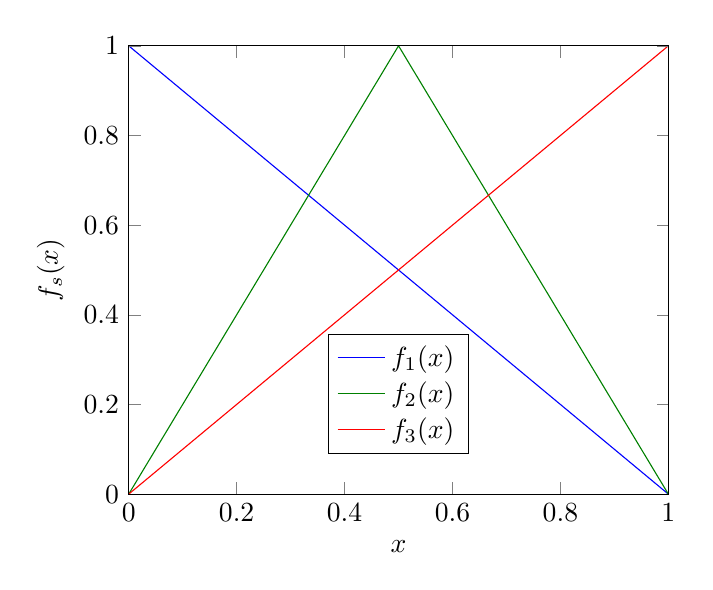
\begin{tikzpicture}
	
	\begin{axis}[
	xlabel={$x$},
	ylabel={$f_s(x)$},
	xmin=0, xmax=1,
	ymin=0, ymax=1,
	axis on top,
	legend style={at={(0.5,0.09)}, anchor=south},
	legend entries={{$f_1(x)$},{$f_2(x)$},{$f_3(x)$}},
	legend cell align={left}
	]
	\addplot [blue]
	table {%
		0 1
		0.5 0.5
		1 0
	};
	\addplot [green!50.0!black]
	table {%
		0 0
		0.5 1
		1 0
	};
	\addplot [red]
	table {%
		0 0
		0.5 0.5
		1 1
	};
	\end{axis}
	
	\end{tikzpicture}
	\caption{Operation of the Centre-Point Triangular Whitenization used in \gls{mtfm}}
	\label{fig:whitenization}
\end{figure}

In the case of the terrestrial communications network used in~\cite{Guo11}, the observed metric set $X = {x_1,\dots,x_M}$ representing the measurements taken by each node of its neighbours at least interval, is defined as $X=[$packet loss rate, signal strength, data rate, delay, throughput$]$.

\citet{Guo11} demonstrated that when compared against \gls{otmf} and Hermes trust assessment, \gls{mtfm} provided increased variation in trust assessment over time, providing more information about the nodes' behaviours than packet delivery probability alone can.

\section{Conclusion}
In this chapter, \gls{manet} implementations, topologies, and applications have been explored. 
Further, the concept of a ``Trusting'' network has been explored, both on a abstract theoretical basis, and in the context of a wider development and operational pipeline involving autonomous actors, including a review of current \acrfullpl{tmf}.
These \glspl{tmf} have several aspects that are dependant on assumptions of sufficient available resources and connectivity, that they may not behave as efficiently as would be hoped in constrained or delayful networks, particularly in cases where metric assessment data may be extremely sparse or noisy.

While many aspects of this Trust have been discussed, we are primarily concerned with this problem of assessment of trust through experiential observation of node behaviours in a practical runtime environment, namely the underwater acoustic environment.
In the next chapter, the marine communications environment will be studied, as will the current state of the art in the use of autonomy in defence related maritime applications, and briefly discussing the context of those operations.
%%%%%%%%%%%%%%%%%%%%%%%%%%%%%%%%%%%%%%%%%%%%%%%%%%%%%%%%%%%%%%%%%%%%%%%%%%%%%%%
 % Background on Trust and its Applications to MANETs

% !TeX spellcheck = en_GB
\chapter{Maritime Communications and Operations}
\label{ch:maritime_background}
\lhead{Chapter \thechapter. \emph{\nameref{ch:maritime_background}}}

\section{Maritime Communications Environment}\label{sec:marine_comms}

The key challenges of underwater acoustic communications are centred around the impact of slow and differential propagation of energy (RF, Optical, Acoustic) through water, and it's interfaces with the seabed / air.
The resultant challenges include; long delays due to propagation, significant inter-symbol interference and Doppler spreading, fast and slow fading due to environmental effects (aquatic flora/fauna; surface weather), carrier-frequency dependent signal attenuation, multipath caused by the medium interfaces at the surface and seabed, variations in propagation speed due to depth dependant effects (salinity, temperature, pressure, gaseous concentrations and bubbling), and subsequent refractive spreading and lensing due to that same propagation variation\cite{Partan2006}.

\subsection{Mechanics of Acoustic Transmission}

Unlike in RF energy transfer (where photons move through space to transmit energy from one place to another), acoustic waves are the result of mechanical perturbation of a medium where localised compressions and extensions pass energy across a medium through that mediums elastic properties.
These ``compression waves'' propagate away from its source, and the rate of this propagation is the sound speed, velocity or $c$, measured in $ms^{-1}$.
This is not to be confused with the fluid velocity corresponding to the instantaneous motion of particles in the medium.

Hydrophones, like their more common microphone equivalent in air, are fundamentally pressure sensors.
Acoustic pressure is usually measured in \emph{Pascals} ($Pa/\mu Pa$). 
In the underwater environment, the dynamic range (difference between instantaneous high and low pressure values) may be extremely high, often more than 10 orders of magnitude higher. 
As such, logarithmic notation is justified.

Useful acoustic signals are generally maintained vibrations rather than instantaneous pulses.
They are characterised by their frequency $f$ expressed in Hertz ($Hz$) or by their Period ($T$) in seconds.
In commonly used underwater acoustics, used frequencies range from $\approx 10Hz-100kHz$ depending on application~\cite{Stojanovic2007}.

As with all waves, the relationship between frequency, period and the wavelength is given as in \eqref{eq:wavelength}. 
As such the generally used upper and lower bounds of wavelength in most applications is from $\SI{1.5}{\meter} @ 10Hz$ to $\SI{0.015}{\meter} @ 100kHz$.
%
\begin{equation}
  \lambda = cT = \frac{c}{f}
  \label{eq:wavelength}
\end{equation}
%

This wide range of frequencies and wavelengths allow for a diverse set of constraining factors; (Paraphrased from~\citet{lurton2010}).

\begin{itemize}
  \item \emph{Attenuation} in water; limiting the maximum usable range, which increases very rapidly with frequency
  \item \emph{Dimensions} of sound source; which increase at lower $f$ for a given transmission power
  \item \emph{Spatial Selectivity} of sources and receivers as $f$ increases, due to similarly increasing directivity of energy propagation.
  \item \emph{Acoustic Response} of target surfaces (analogous to receiver gain in RF networks).
\end{itemize}

\subsection{Velocity and density}\label{sec:aco_vel}

Air has a baseline density of approximately $\SI{1.3}{\kilogram\per\meter\cubed}$, and the speed of sound is typically static around $\SI{340}{\meter\per\second}$.
In sea water, acoustic wave velocity is close to $c=\SI{1500}{\meter\per\second}$ (generally between $\SIrange{1450}{1550}{\meter\per\second}$ depending on temperature, pressure, salinity etc.).
Similarly variable is sea water density, which is nominally $\rho = \SI{1027}{\kilogram\per\meter\cubed}$\cite{Wang2010}.

While the sea/air surface is (ideally) a simple refractive interface, the interface between open seawater and marine sediment is graduated, with density ranges between $\SIrange{1200}{2000}{\kilogram\per\meter\cubed}$. 
This results in refractive and reflective velocities in the sediment interface ranging from $\SIrange{1500}{2000}{\meter\per\second}$\cite{lurton2010}.

For comparison, the speed of light in air/water is $\SI{2.99e8}{\meter\per\second}$ and $\SI{2.249e8}{\meter\per\second}$ respectively. 

\begin{table}
	\centering
	\caption{Summary of physical factors differentiating terrestrial and acoustic channel constraints}
	\label{tab:channel_constraings_comp}
	\begin{tabularx}{0.8\textwidth}{X X X}\toprule
		Variable & Air & Water\\
		\midrule
		Density & $\SI{1.3}{\kilogram\per\meter\cubed}$ & $\approx\SI{1027}{\kilogram\per\meter\cubed}\pm0.5\%$ \\
		Speed of Sound & $\SI{340}{\meter\per\second}$ & $\approx\SI{1500}{\meter\per\second}\pm 5\%$ \\
		Speed of Light & $\SI{2.99e8}{\meter\per\second}$ & $\SI{2.249e8}{\meter\per\second}$\\
		\bottomrule
	\end{tabularx}
\end{table}
\citet{Mackenzie1981} proposed a more accurate model of acoustic velocity incorporating archival data from 15 worldwide sites that takes Temperature, Salinity and Depth into consideration.

\begin{align}
  c = & 1448.96 + 4.591 T - 5.304 \times 10^{-2} T^2 + 2.374 \times 10^{-4}T^{3}\notag\\
  & +1.340 (S-35) + 1.630\times 10^{-2}D+1.675\times 10^{-7}D^2\\
  & -1.025 \times 10^{-2}T(S-25) - 7.139\times 10^{-13}TD^3\notag
  \label{equ:mackenzie}
\end{align}

Where $T$ is the temperature in Celsius, $S$ the salinity in parts per thousand, and $D$ is the depth below the surface in meters.

\begin{figure}
	\centering
	\begin{subfigure}[t]{0.8\textwidth}
		\centering
		\includegraphics[width=\textwidth]{temp_globe}
		\caption{Surface Temperature}
		\label{fig:temp_globe}
	\end{subfigure}
	\begin{subfigure}[t]{0.8\textwidth}
		\centering
		\includegraphics[width=\textwidth]{sal_globe}
		\caption{Surface Salinity}
		\label{fig:sal_globe}
	\end{subfigure}
	\caption{Global Variations in selected Speed of Sound variance factors}
	\label{fig:globes}
\end{figure}

These are ``ideal'' assessments, and the parameters of this model are massively varied both across individual water columns, and indeed across bodies of water, across the world. 
\gls{noaa} regularly publish their \gls{woa}~\cite{Locarnini2013,Zweng2013} that includes these variables and many more, sampled across the world and at a range of depths. 
Outputs from these surveys are shown for example in \autoref{fig:globes}. 
Variability in Temperature across the globe is something that we are acutely aware of, but the significant regional variations, such as in the Sea of Japan, the US Eastern Seaboard, and between the Mediterranean and Black Seas (\autoref{fig:temp_globe}).
Global surface salinity appears almost uniform in comparison (\autoref{fig:sal_globe}).
However, a few global variants stand out, both due to the extremity of their transition in relatively small areas, and the general research / defence context of those areas. 
For example the differential between the geographically proximate and politically contentious Black, Caspian, and Mediterranean Seas, as well as the Persian Gulf exhibit variations from less than $6ppt$ to over $40ppt$.
Similarly, there is a navigable waterway providing access between the Baltic and North seas that across the $\SI{300}{\kilo\meter}$ long run from Malm{\"o} in Sweden to Skagen in Denmark, transitions from less than $5ppt$ to just under $30ppt$. 

Below the surface, the variability increases; \autoref{fig:temp_sal_profile} shows an example of a depth profile of these variations and the modelled impact on the speed of sound with respect to depth in three different regions. 
The variability of this speed is crucial to the operation of an underwater acoustic network, as it fundamentally changes the propagation paths of compressive energy transfer, and in particular, the fastest ``path''. 
\autoref{fig:ssps} shows the impact on this fastest recieved path and it's true path between two nodes in shallow, littoral, waters.
Even with relatively small variations in sound speed, and with the introduction of sea floor/surface interfaces, the ``fastest'' path deviates significantly from a true ``line of sight'' path where there is any variability in speed of sound profile, making delay-based positioning extremely difficult, and presents significant opportunities for out-of-sync multi-path effects\footnote{\autoref{fig:ssps} shows a staged, iterative approximation method to arrive at the shortest path, where the ``colour intensity'' of the chart shows the stage at which that path was explored, so the ``final'' paths are darkest, and the ``exploitative'' paths are lightest, however in reality these secondary paths are still emitted and arrive, delayed, to the reciever, causing significant inter-symbol interference unless equalised.}



\begin{figure}
	\centering
	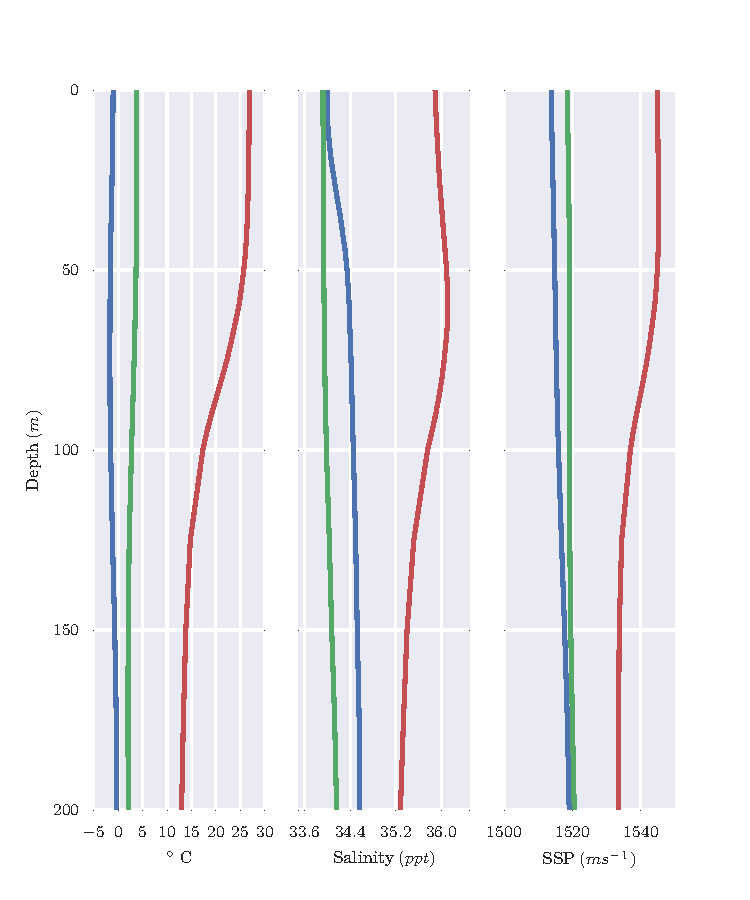
\includegraphics[height=6in]{temp_sal_profile}
	\caption{Depth Variations in selected Speed of Sound variance factors}
	\label{fig:temp_sal_profile}
\end{figure}


\begin{figure}
	\begin{subfigure}[t]{0.45\textwidth}
		\centering
		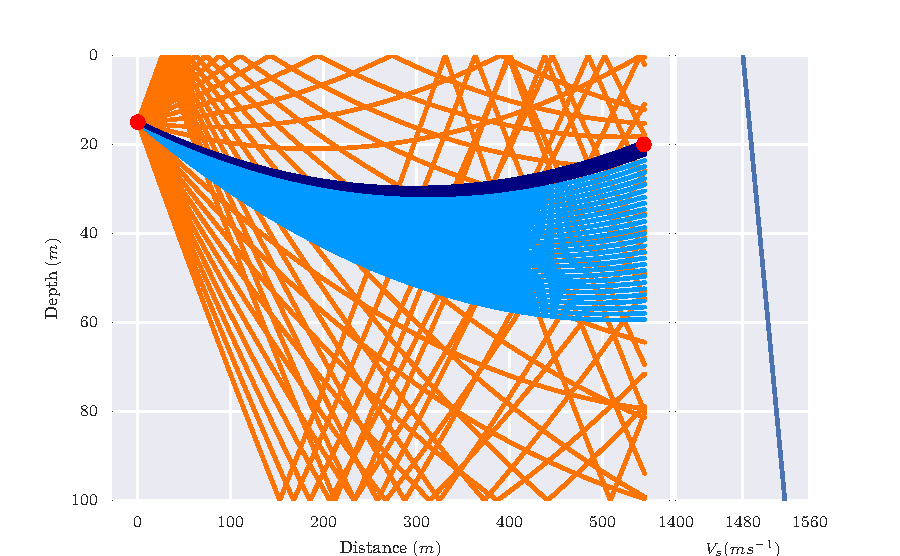
\includegraphics[width=\textwidth]{ssp_linear_increasing}
		\caption{Linear Increasing}
		\label{fig:ssp_linear_increasing}
	\end{subfigure}
	\begin{subfigure}[t]{0.45\textwidth}
		\centering
		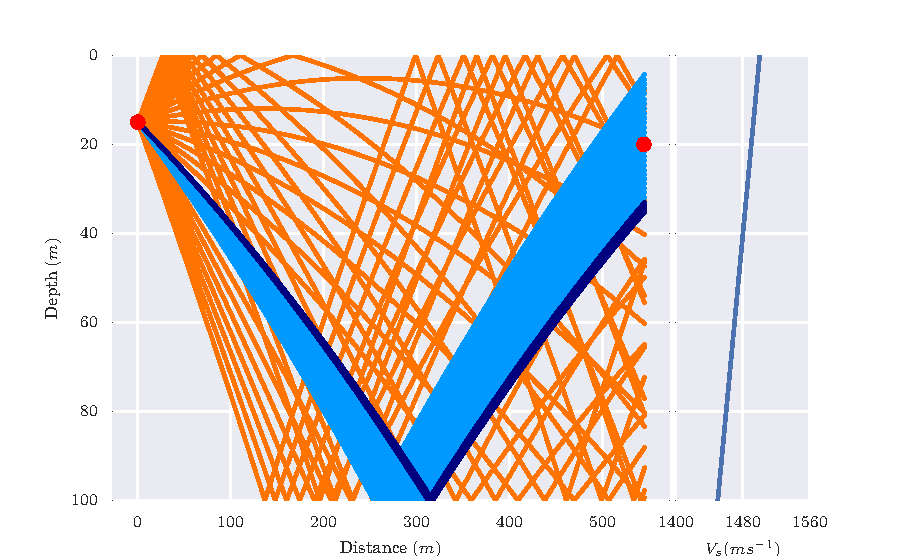
\includegraphics[width=\textwidth]{ssp_linear_decreasing}
		\caption{Linear Decreasing}
		\label{fig:ssp_linear_decreasing}
	\end{subfigure}\\
	\begin{subfigure}[t]{0.45\textwidth}
		\centering
		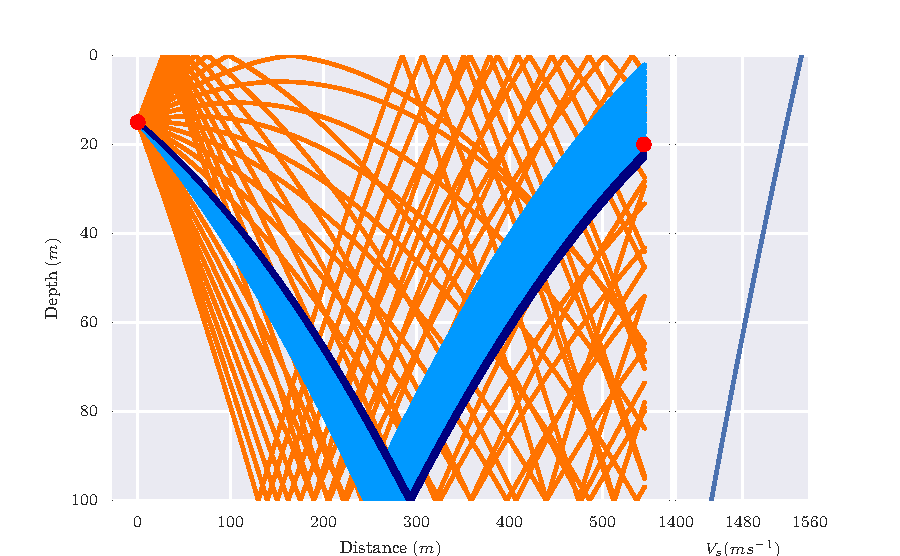
\includegraphics[width=\textwidth]{ssp_n_squared}
		\caption{Quadratic}
		\label{fig:ssp_n_squared}
	\end{subfigure}
	\begin{subfigure}[t]{0.45\textwidth}
		\centering
		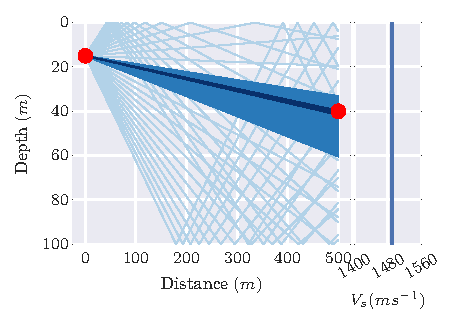
\includegraphics[width=\textwidth]{ssp_isovelocity}
		\caption{Isovelocity}
		\label{fig:ssp_isovelocity}
	\end{subfigure}
	\caption{Bellhop Model of Non-Linear Marine Shortest-Path Propagation in various Speed of Sound Profiles}
	\label{fig:ssps}
\end{figure}

\subsection{Intensity and Power} 

The energy of an acoustic wave is encapsulated into its kinetic and potential parts; where its kinetic energy corresponds to the active motion energy of the particles in the medium, and the potential energy corresponding to the elastic potential of the medium in displacement/compression.

The acoustic intensity ($I$) is the energy flux mean value per unit of surface and time \eqref{eq:acoustic_intensity} in Watts/$m^2$ where $p_0$ is the plane wave amplitude (pressure) and $P_{rms} = p_0/\sqrt{2}$

\begin{equation}
  I = \frac{p_0^2}{2\rho c} = \frac{p_{rms}^2}{\rho c}
  \label{eq:acoustic_intensity}
\end{equation}

\subsection{Attenuation}

The attenuation that occurs in an underwater acoustic channel over a distance $d$ for a signal about frequency $f$ in linear \eqref{eq:acoattenuation} and $dB$ forms \eqref{eq:acoattenuationdb} is given as;

\begin{equation}
  \label{eq:acoattenuation}
  A_{\text{aco}}(d,f) = A_0d^ka(f)^d
\end{equation}
\begin{equation}
  \label{eq:acoattenuationdb}
  10 \log A_{\text{aco}}(d,f)/A_0 = k \cdot 10 \log d + d \cdot 10 \log a(f)
\end{equation}

where $A_0$ is a unit-normalising constant, $k$ is a geometric spreading factor (commonly taken as 1.5 for practical use, but may be 2 for perfect spherical propagation or 1 for perfect plane-wave propagation)), and $a(f)$ is the absorption coefficient, that may be modelled in a variety of ways.

Thorp's formula (\autoref{eq:thorp}) is very simple, only depending on $f$, and is designed to be most accurate about a temperature of 4$^{\circ}$C at a depth of $\approx 1Km$.
%
\begin{figure}
  \begin{equation}
    10 \log a(f) = 0.11 \cdot \frac{f^2}{1+f^2} + 44\cdot\frac{f^2}{4100+f^2}+ 2.75\times10^{-4} f^2 + 0.003
    \label{eq:thorp}
  \end{equation}
  \caption[Thorp's formula]{Thorp's Absorption Model~\cite{Stojanovic2007}}
    \label{fig:thorp}
\end{figure}
%
The Ainslie \& McColm model is more complex, and incorporates the acidity of the water ($H^+$) as well as temperature ($T$), salinity ($S$ in parts per trillion) but not depth (\autoref{fig:ainslie}).
%
\begin{figure}
  \begin{align}
    10 \log a(f) =& 0.106 \frac{t_1 f^2}{t_1^2 + f^2} e^{\frac{H^+-8}{0.56}}\\\notag
      & + 0.52 \left(1+\frac{T}{43}\right)\left(\frac{S}{35}\right)\frac{t_2f^2}{t_2^2+f^2} e^{\frac{-D}{6}}\\\notag
      & + 4.9 \times 10^{-4} f^2e^{-\left(\frac{T}{27}+\frac{D}{17}\right)}\\\notag
      \text{Where}&\\\notag
      t_1 =& 0.78 \sqrt{\frac{S}{35}e^{\frac{T}{26}}}\\\notag
      t_2 =& 42 e^{\frac{T}{17}}\notag
      \label{eq:ainslie}
  \end{align}
  \caption{Ainslie \& McColm Absorption Model}
  \label{fig:ainslie}
\end{figure}
%
\begin{figure}
  \begin{align}
    10 \log a(f)=& A_1P_1\frac{t_1f^2}{t_1^2+f^2} + A_2P_2\frac{t_2f^2}{t_2^2+f^2} + A_3P_3f^2\\\notag
    \text{Where }&\\\notag
    A_1=&1.03\times 10^{-8} + 2.36\times 10^{-10} \cdot T -5.22 \times 10^{-12}\cdot T^2\\\notag
    A_2=&5.62\times 10^{-8} + 7.52\times 10^{-10} \cdot T\\\notag
    A_3=&\left(55.9 - 2.39\cdot T + 4.77\times 10^{-2}\cdot T^2 - 3.48 \times 10^{-4}\cdot T^3\right) \times 10 ^{-15}\\\notag
    t_1=&1.32\times 10^3\left(T+273.1\right)e^{\frac{-1700}{T+273.1}}\\\notag
    t_2=&1.55\times 10^7\left(T+273.1\right)e^{\frac{-3052}{T+273.1}}\\\notag
    P_1=&1\\\notag
    P_2=&\-10.3\times 10^{-4}\cdot P + 3.7\times 10^{-7}\cdot P^2\\\notag
    P_3=&\-3.84\times 10^{-4}\cdot P + 7.57\times 10^{-8}\cdot P^2\notag
    \label{eq:fisher}
  \end{align}
  \caption{Fisher-Simmons Absorption Model}
  \label{fig:fisher}
\end{figure}
%
The Fisher-Simmons model (\autoref{fig:fisher}) is significantly more complex, taking into account the effects of boric acid concentrations and dissolved magnesium sulphate. While there are several limitations on this model in terms of its being fixed at a salinity of 35 ppt and a pH of 8, as this model incorporates depth, temperature, distance and frequency, it is very attractive for research directed at high variability environments and is used for the remainder of this work unless otherwise stated.

%\todo{Possibly need to switch this with the Francois Garrison model which, depending on your source, is the refined version (or vise versa}



Regardless of the variations of particular attenuation models, comparing $A_{aco}(d,f)$ with the RF Free-Space Path Loss model~\autoref{eq:fspl}, the impact of range on signal power is exponential underwater, rather than quadratic in terrestrial RF ($A_{\text{aco}} \propto f^{2d}$ vs $A_{\text{RF}} \propto (df)^2$). 
While both frequency dependant factors are quadratic, approximating the factors in \eqref{eq:thorp}, $f\propto A_{\text{aco}}$ is at least 4 orders of magnitude higher than $f\propto A_{\text{RF}}$
\begin{equation}
  \label{eq:fspl}
  A_{\text{RF}}(d,f) \approx \left( \frac{4\pi d f}{c} \right)^2
  \text{where }c\approx \SI{3e8}{\meter\per\second}
\end{equation}


 \subsection{Ambient Noise Model}

 Ambient ocean noise can be assumed to be Gaussian with a continuous power spectral density in dB re $\si{\micro\pascal\per\hertz}$, driven by four major factors, shown in \autoref{tab:ocean_noise_factors}, where $s$ is a shipping activity factor bounded from $[0,1]$ and $w$ is the surface wind speed in $\si{\meter\per\second}$~\cite{coates1989}.

\begin{table}[h]\centering
  \caption{Contributing factors to Ocean Ambient Acoustic Noise}
  \label{tab:ocean_noise_factors}
  \begin{tabularx}{\textwidth}{p{3.5cm} X}\toprule
    Source & Approximation \\ \midrule
    Turbulence & $10 \log N_t(f)=17-30\log f$\\
    Shipping & $10 \log N_s(f) = 40+20(s-0.5)+26\log f-60\log(f+0.03)$\\
    Wind Driven Waves & $10\log N_w(f) = 50+7.5w^{\frac{1}{2}}+20\log f - 40\log(f+0.4)$\\ 
    Thermal Noise & $10\log N_{th}(f) = \-15 + 20 log f$\\\bottomrule
  \end{tabularx}
\end{table}

\subsection{Multipath effects}

Refractive lensing and the multi-path nature of the medium result in line of sight propagation being extremely unreliable for estimating distances to targets (See \autoref{sec:aco_vel} and \autoref{fig:ssps}).
The first arriving acoustic signal has as the very least curved in the medium, and commonly has reflected off the surface/seabed before arriving at a receiver, creating secondary paths that are sometimes many times longer than the first arrival path, generating symbol spreading over orders of seconds depending on the ranges and depths involved.
Thus, the multi-path channel transfer function can be described by :

\begin{align}
  \label{eq:acomultipath}
  H(d,f) =\sum_{p=0}^{P-1} h(p) = \sum_{p=0}^{P-1} \Gamma_p / \sqrt{A(d_p,f)}e^{-j 2 \pi f \tau_p} \\
  \text{where } \tau_p = d_p/c, c \approx \SI{1500}{\meter\per\second} \notag
\end{align}

where $d=d_0$ is the minimal path length between the transmitter and receiver, $d_p,p=\{1,\dots P-1\}$ are the secondary path lengths, $\Gamma_p$ models additional losses incurred on each path such as reflection losses at the surface interface, and $\tau_p = d_p/c$ is the delay time.


\subsection{Modelling and Simulation of the Acoustic Medium / Channel}

Several toolkits exist in a variety of states that perform communications agent simulation, most notably the NS-2 / 3 family of frameworks and their add-ons.
Some of these frameworks, such as SUNSET~\cite{Petrioli2012a} and AquaTools~\cite{Sehgal2010}, that are particularly proven in their capability in modelling static network performance, with less in built support for advanced, reactive node mobilities such as those involving collision or object avoidance.

Beyond the NS family, there are many other communications and simulation modelling systems such as OpNet++~\cite{Chang1999} and MATLAB toolkits such as the AcTUP interface to the Ocean Acoustics Library, that primarily focus on simulation of the acoustic channel and contention issues without concentration on Underwater-specific \gls{mac} protocols.

AUVNetSim is a simulation platform designed from the ground up with \gls{auv} operations in mind~\cite{Miquel2008}.
Including support for dynamic modular mobility and application behaviours, considering the stated context of an environmentally reactive \gls{uan}, AUVNetSim was tested and selected as a foundation upon which to build an exploratory network testing framework for this research.

In order to implement a collaborative, reactive, simulation suite, the SimPy~\cite{Mueller2003SimPy} agent framework was used for ``background'' synchronisation.

As mentioned in the individual testing cases, transmission parameters for simulation were initially taken from and validated against results from~\citet{Stojanovic2007} and~\citet{Stefanov2011}.


\begin{comment}
\subsection{Routing and Network Design for \glspl{uan}}

Forward Error Correction coding is used on such channels to minimise packet losses.

\todo{ADD:Summary of Akyildiz02/05}

\todo{FIX:callback to routing discussion in c1 explain why fbr is the best of everything all the time}
\end{comment}

\section{Marine Operations, Payloads, Technologies, and Durations}\label{sec:marine_ops}

The use and applications of \glspl{auv} has undergone a great expansion in recent years~\cite{Alam2014}.
The primary application for \glspl{auv} has long been identified as the environmental monitoring of marine areas, and are actively being researched by a great range of industrial and defence sector applications, with secondary applications in the physical sciences and environmental research, which are summarised below\cite{Bingham2002,Wynn2014}.

\subsection{\gls{auv} operations and deployments}

\subsubsection{Hydrographic Survey}

The use of \glspl{auv} in the place of manned-surface platforms or tethered undersea platforms enables greatly increased spatial and temporal sampling.
Importantly, the separation of \glspl{auv} from the noisy sea surface enables much more efficient survey operations.
This is particularly important when comparing to classical tow-line based measurements; where the mobility of the \glspl{auv} enables for much tighter-turning survey patterns or operation in inaccessible or hard-to-reach locations such as polar survey~\cite{Curtin1993}.

Another significant factor is cost; the daily cost of operating a manned vessel can be considerably higher than the costs of deploying, operating and recovering one or more \glspl{auv} with equivalent capabilities~\cite{Nicholson2008}.
Additionally, the use of low-power ``glider'' \glspl{auv} has lowered the barrier to entry for extended mission types, such as persistent environmental survey, or open-ocean operations. 
Depth-hardened \glspl{auv} have also opened up the deepest parts of the oceans to exploration, with the onboard autonomy, imagery and Simultaneous Location and Mapping (SLAM) techniques allowing deep-dwelling survey \glspl{auv} to react to bottom-surface features without the need for a tight craft-to-surface control loop.
The natural extension of these kind of applications is the use of \glspl{auv} on ice-covered planets such as Europa, where three-dimensional, autonomous navigation without an on-the-loop controller is vital for mission resource efficiency and success.

\subsubsection{Hull and Infrastructure Inspection}
Ongoing concerns regarding the security, safety and legality of international shipping has driven the application of \glspl{auv} to the area of near-surface hull and infrastructure inspections, looking for damage as well as devices such as limpet mines and other contraband.
This use case puts a range of unique pressures on the \gls{auv} system; requiring highly accurate three-dimensional localisation and path-planning to clearly image the contours of a hull~\cite{Nicholson2008}.
Similarly, with the increasing use and criticality of intercontinental undersea optical fibre connections, using \glspl{auv} for both the laying of and inspection of these cables is an exciting area of work~\cite{Yu2004,Asakawa2002}.

\subsubsection{Marine Petrochemical/Mineralogy}
Oil and Gas industry requirements for high quality, low altitude bathymetry of seabed structures for infrastructure development (pipelines/drill platforms etc.) as well as monitoring of those structures over time (inspection etc.) is another significant application area, and a major driver of research investment.
As in Hydrography, the mobility of \glspl{auv} is the biggest single advantage over classical platforms~\cite{Morr2003}.
Additionally, recent advances in \gls{sas} have provided invaluable sub-surface profile data over much wider areas for multi-spectral mineralogical analysis than previous sonar profilers~\cite{Denny2015}.

\subsubsection{Military}
\gls{mcm} Operations benefit greatly from, and significantly drive, \gls{auv} development; the ability to rapidly explore and covertly survey a potentially dangerous area without risking a human operator is a major benefit both in Dedicated \gls{mcm} (e.g. Large Area Hunting/ \gls{eod} Clearance) and in Organic \gls{mcm} for Expeditionary Forces.
This benefit applies to protection as well as incursion; the ability to rapidly deploy persistent survey of a valuable area such as a forward-operating harbour is increasingly essential, and as \gls{auv} technology, autonomy and security practices develop, this use is increasing.
This Port Protection capability is particularly complex;  teams of \glspl{auv} are expected to repeatedly survey an area and remain densely-connected enough to maintain end-to-end communications with all other nodes, in the face of an environment that is possibly not well surveyed initially, and includes dynamically moving obstacles (i.e.\ ships).
In the remainder of this work this Port Protection scenario is used as a baseline for our simplified simulation context.
Additional defence application areas include \gls{asw}, \gls{rea}, Navigational Aid/Force projection, 



\subsection{Localisation Technologies}

Given the subsurface nature of most \gls{auv} operations, terrestrial localisation techniques such as \gls{gps} are unavailable (below $\approx 20cm$ depth). 
However, a range of alternative techniques are used to maintain spacial awareness to a high degree of accuracy in the underwater environment.
\subsubsection{\gls{lbl}}
Long-baseline localisation systems use a series of static surface/cable networked acoustic transponders to provide coordinated beacons and (usually) \gls{gps}-backed relative location information to local subsurface users. 
Such systems can be accurate to less that $0.\SI{1}{\meter}$ or better in ideal deployments and are regularly used in controlled autonomous survey environments such as harbour patrol operations where the deployment area is bounded. 
However, the initial set-up and deployment required in advance of any \gls{auv} operation makes \gls{lbl} difficult to utilise in unbounded or contended areas.
\gls{lbl} systems can also be deployed on mobile surface platforms in the area (ships or buoys for example), but these applications put significant computational pressure on the end-point AUV and have greatly reduced accuracy compared to ideal deployments~\cite{Matos1999}.
\subsubsection{\gls{dvl}}
Doppler Velocity Logging involves the emission of directed acoustic ``pings'' that reflect off sea bed/surface interfaces that, when received back on the craft with multi-beam phased array acoustic transducers can measure both the absolute depth/altitude (z-axis) of the craft and through directional Doppler shifting, the relative (xy-translative) motion of the craft since the ping.
While classical \gls{dvl} was highly sensitive to shifting currents in the water column, advances in the development of Acoustic Doppler Current Profiling has turned that situation on it's head, enabling the compensation-for and measurement-of water currents down to the sub-meter level~\cite{Snyder2010}.
\subsubsection{\gls{ins}}
Inertial navigation systems use gyroscopic procession to observe the relative acceleration of a mobile platform.
This reference-relative monitoring is particularly useful in the underwater environment, as it detects the motion of \glspl{auv} as they are carried by the water itself.
Bias Drift is a significant problem for \gls{ins} systems operating over longer (hundreds of metres) distances, as they usually have some minimal amount of directional bias, that incurs a cumulative effect over time without assistance.
Several sensor synthesis processes have been demonstrated which combine information from \gls{ins} along with \gls{dvl} data to improve localisation into the sub-decimeter level~\cite{Jalving2003,Liu2014,Allotta2015}.
\subsubsection{\gls{slam}}
Simultaneous Location and Mapping is the process of iteratively developing a feature-based model of an environment, and to use the relative movement within that modelled environment to obtain estimates of absolute positioning.
\gls{slam} has been most well developed in the contexts of either visual-based inspection using cameras, or LIDAR-style distance triangulation, however the same principles have been successfully applied using marine sonar readings, providing sub-meter accuracy, real-time, feature-relative localisation information that is (for the most part) environmentally agnostic~\cite{Williams2000}.

\vspace{\baselineskip}

In summary, current technology reliably enables \glspl{auv} to localise to a sub-metre accuracy in most areas of application.

\subsection{Example Maritime Autonomous Systems, Platforms and Operational Limitations}

\subsubsection{Kongsburg REMUS/HUGIN ranges}

The REMUS range of \gls{auv} platforms have been very popular in research and \gls{uan} application prototypes due to their relatively small size and high level of reconfigurability.
The basic configurations of the REMUS 100 configuration consist of a single pressure vessel, $\SI{0.2}{\meter}$ in diameter and $\SI{1.6}{\meter}$ long, weighting in at $37kg$, rated to operational depths of $\SI{150}{\meter}$. 
This package includes \gls{dvl}, \gls{ctd}, Underwater Videography, \gls{lbl} and onboard computing power suitable for low \gls{loa} independence, with onboard Li-on battery packs rated to provide up to 10-hours of cruising operational endurance.
These capabilities can be extended through the addition of further modular extensions through the REMUS range, such as the REMUS 600, rated for up to $\SI{600}{\meter}$ depth and a cruising endurance of 45 hours, or the REMUS 6000, rated for up to $\SI{6}{\kilo\meter}$ with 22 hours duration.

The HUGIN 1000 is a high-resolution extension to the REMUS range, characterised by it's default payload of a High Definition \gls{sas}, co-designed with the Norwegian Defence Research Establishment (FFI) for \gls{mcm} operations, with a dynamic depth rating up to $\SI{3}{\kilo\meter}$ and 24 hour cruising endurance (17 hours with continuous \gls{sas} engagement)

The Konsburg range also include range specific \gls{lars}
\begin{figure}[h]
	\centering
	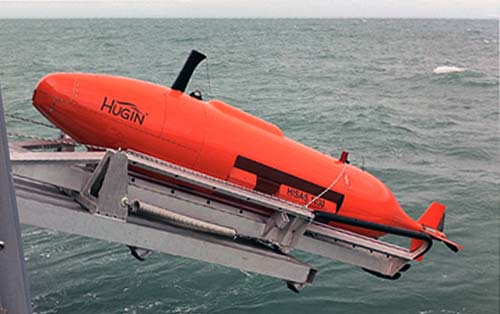
\includegraphics[width=0.45\textwidth]{hugin.jpg}
	\caption{\label{fig:hugin}HUGIN AUV mounted on LARS}
\end{figure}
\subsubsection{NOC Autosub}

Developed under the UK's National Oceanography Centres Marine Autonomous and Robotic Systems group, the Autosub family of \glspl{auv} is similar in many ways to the REMUS deployment profile; with long range and deep-ocean variants, operating at depths up to \SI{600}{\kilo\meter} for up to 36 hours (however, this configuration leaves it with a cruising speed of \SI{0.4}{\meter\per\second})
\begin{figure}[h]
	\centering
	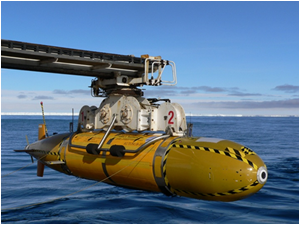
\includegraphics[width=0.45\textwidth]{autosub}
	\caption{\label{fig:autosub}NOC Autosub 3 being deployed off the Pine Island Glacier}
\end{figure}

\subsubsection{University of Washington SeaGlider}
Taking a fundamentally different approach to underwater mobility for targeting depth-variant environmental studies, the SeaGlider eschews classical propulsion to use it's downward-facing structure and fins to use it's weight/buoyancy to propel itself.   
At \SI{1.8}{\meter} long and weighting only \SI{52}{\kilogram}, this highly portable \gls{auv} can cover ranges up to \SI{4600}{\kilo\meter} with 650 \SI{1}{\kilo\meter} dive segments at a rate of \SI{0.25}{\meter\per\second}.
\begin{figure}[h]
	\centering
	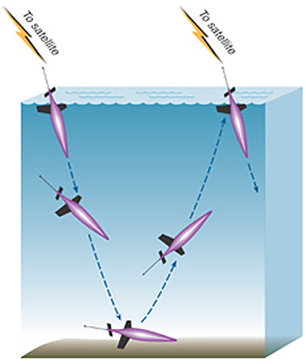
\includegraphics[width=0.45\textwidth]{seaglider}
	\caption{\label{fig:seaglider}''Flight path'' of the UW SeaGlider}
\end{figure}

\subsubsection{USN Sea Hunter}
The Sea Hunter is an autonomous unmanned surface vehicle (USV) launched in 2016 and is undergoing seatrials as part of the \gls{darpa} Anti-Submarine Warfare Continuous Trail Unmanned Vessel program, with a top speed of \SI{50}{\km\per\hour}, weighing \SI{122}{\tonne}.
While unarmed during its sea trials, the \emph{Sea Hunter} will be armed and used for \gls{asw} and \gls{mcm} duties, operating at a tiny fraction of the standard operating costs of a littoral destroyer.
\begin{figure}[h]
	\centering
	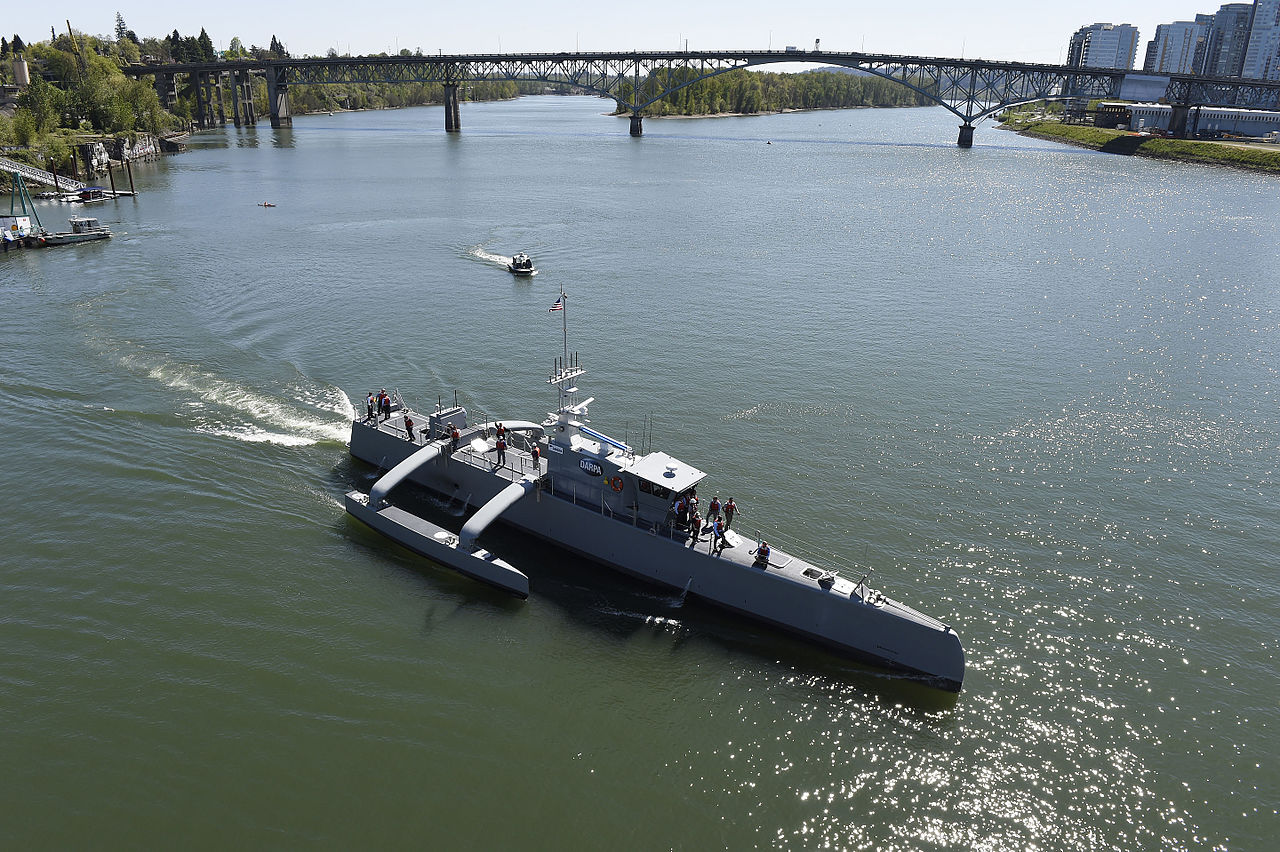
\includegraphics[width=0.45\textwidth]{seahunter}
	\caption{\label{fig:seaglider}Initially manned deployment of the unmanned \emph{Sea Hunter}. U.S. Navy photo by John F. Williams/Released}
\end{figure}

\subsection{Need for Trust in Maritime Networks}\label{sec:trust_in_marine}


Given the breadth of the threat space in \glspl{manet}, many strategies for mitigating these risks have been proposed in a matrix-basis; i.e. you can't cover all eventualities with one tool.
\autoref{tab:manet_risk} summaries some of these general strategies or ``solutions'' for range of threats identified specifically in the context of the deployment of \glspl{manet} in a tactical/defence context, originally based on~\citet{Kidston2010} but with some contextual alterations with modifications discussed below.

In this context of this table, Vulnerability is an assessment of how available a particular threat is to a generic attacker, Impact is an assessment of the in-system affects of a successful attack, and Risk is a qualitative assessment of the likelihood of exploitation of an attack.
\citet{Kidston2010} originally lowered the assessment of vulnerability of Eavesdropping, citing the tactical use of non-standard \gls{mac} as a barrier to attack, however considering the increasing commoditisation of tactical hardware across the world, and increasing application of \gls{cots} hardware, this is no longer a fair assessment.
Similarly, the assessment that the Risk of Data Corruption is low is arguable on the basis of simplistic spread spectrum jamming but this assessment is unchanged.
%Finally,~\citet{Kidston2010} did not take into account the presence of weapons or other actuation methods with \glspl{auv} as the endpoint.

\begin{table}
	\caption{Risks and Threat Mitigation Strategies for \glspl{manet}, extended from~\cite{Kidston2010}}
	\label{tab:manet_risk}
	\begin{tabularx}{\textwidth}{p{4cm} X X X >{\raggedright\arraybackslash}p{4cm}}\toprule
		Threat & Vulnerability & Impact & Risk & Mitigation	\\\midrule
		Resource Depletion / \gls{dos} & Low-High & High & Low-High & Layer Specific Mechanisms~\cite{Wu2007,Nwaocha2015}\\
		Eavesdropping & Medium & High & Low & Cryptography~\cite{Chen2010}\\
		Masquerade & Low & Very High & Medium & Trust Systems and Cryptography~\cite{Wang2009a}\\
		Data Corruption & Low & High & Low & Cryptography\\
		Traffic Analysis & High & Low & Medium & Obfuscation~\cite{Huang2010}\\
%		Misfire/Misactuation & Low & Very High & High & Man-in-the-loop firing\cite{Caseley2009}\\
	\end{tabularx}
\end{table}

Resource Depletion, or \gls{dos} has a very wide ranging definition, from network-level attacks to saturate a communications channel or the computing resources of routing nodes, or the exploitation of a power-control loop to induce a node to waste energy with overly-high-powered communications, to the intentional geographic misleading of nodes to induce a similar power-drain on locomotive systems, through tactics such as location spoofing or \gls{gps} denial~\cite{Zuba2015}.

From \autoref{tab:manet_risk}, it is assessed that the highest overall threats are those of Resource Depletion and Masquerading.
Within this threat context, the general optimisation of any \gls{tmf} would be to prefer high but fair overall network throughput, while minimising delay, \gls{plr}, and power usage.

\section{Conclusion}

As \acrfull{auv} platforms become more capable and economical, they are being used in many applications requiring trust.
These applications are using the collective behaviour of teams or fleets of these \glspl{auv} to accomplish tasks~\cite{Caiti2011}.
With this use being increasingly isolated from stable communications networks, the establishment of trust between nodes is essential for the reliability and stability of such teams.
In the next chapter, the use of Trust methods developed in the terrestrial \gls{manet} space will be re-appraised for application within the challenging underwater communications channel.

%%%%%%%%%%%%%%%%%%%%%%%%%%%%%%%%%%%%%%%%%%%%%%%%%%%%%%%%%%%%%%%%%%%%%%%%%%%%%%%
 % Background on Maritime Uses of Autonomous Systems and the Maritime Communications Environment

% !TeX spellcheck = en_GB

\chapter{Assessment of \gls{tmf} Performance in Marine Environments}
\label{ch:comms_trust}
\lhead{Chapter \thechapter. \emph{\nameref{ch:comms_trust}}}

\section{\glspl{uan} as \gls{manet} analogue}


As \glspl{manet} grow beyond the terrestrial arena, their operation and the protocols designed around them must be reviewed to assess their suitability to different communications environments to ensure their continued security, reliability, and performance.
With demand for smaller, more decentralised \gls{manet} systems in a range of domains and applications, as well as a drive towards lower per-unit cost in all areas, \glspl{tmf} are increasingly applied to resource constrained applications, as the benefits and efficiencies these systems present are significant.
Many \glspl{uan} use \gls{manet} architectures, however the marine environment presents new challenges for trust management frameworks that have been developed for use in conventional (i.e. Terrestrial RF) \glspl{manet}.
These increasingly decentralised applications present unique threats against trust management \cite{Caiti2011}.

Previous research has established the advantages of implementing \glspl{tmf} in 802.11 based \glspl{manet}, particularly in terms of preventing selfish operation in collaborative systems \cite{Li2007}, and maintaining throughput in the presence of malicious actors \cite{Buchegger2002}

To date this work has been limited to terrestrial, RF based networks, which, as discussed in \autoref{ch:maritime_background}, is a much more favourable communications environment compared to the marine environment of \glspl{uan}, where extreme communications challenges are present (propagation delays, frequency dependent attenuation, fast and slow fading, refractive multipath distortion, etc.).
As a result of these challenges, in underwater environments, communications is both sparse and noisy.
That is to say that long delays create high susceptibility to contention blocking, requiring relatively low channel occupancy and significant back-offs and significant retransmission penalties in the face of a multitude of noise sources over inconsistent, non-linear, multi path transmissions.
Therefore the observations about the communications processes that are used to generate the trust metrics, occur much less frequently, with much greater error (noise) and delay than is experienced in terrestrial RF \glspl{manet}.
Beyond the constraints of the communications environment, knock on pressures in battery capacity, on-board processing, and locomotion simultaneously present opportunities and incentives for malicious or selfish actors to appear to cooperate while not reciprocating, in order to conserve power for instance.
These multiple aspects of potential incentives, trust, and fairness do not directly fall under the scope of single metric trusts discussed previously in \autoref{sec:tmfs}, and this context indicates that a multi-metric approach may be more appropriate.

As such, the use of trust methods developed in the terrestrial \gls{manet} space must be re-appraised for application within the underwater context \cite{Pavan2015}.

This chapter is primarily concerned with the analytical establishment of hard trust within a topologically dynamic network of mobile autonomous actors.
It is shown that single metric trust systems are not directly suitable for the marine context in terms of the different threat and cost scenario in that environment.
These single metric \glspl{tmf} provide malicious actors with a significant advantage if their activity does not impact that metric.

In the case where the attacker can subvert the \gls{tmf}, the metric under assessment by that \gls{tmf} does not cover the threat mounted by the attacker.
This causes a significant negative effect on the efficiency of the network, as the \gls{tmf} is assumed to have reduced the possible set of attacks when it has actually made it more advantageous to attack a different part of the networks operation.
An example of such a situation would be in a \gls{tmf} focused on \gls{plr} where an attacker selectively delays packets going through it, reducing overall throughput but not dropping any packets.
Such behaviour would not be detected by the \gls{tmf}.

For the purposes of this work, from those \glspl{tmf} discussed in~\autoref{sec:tmfs}, Hermes trust establishment, \gls{otmf} and \gls{mtfm} are selected as indicative single and multi metrics frameworks for comparison, as Hermes captures the core operation of a pure single metric assessment methodology and \gls{otmf} provides a comparison that combines assessments from across nodes to develop trust opinions.
\gls{mtfm} is also included as an example of an existing multi-metric \gls{tmf} that looking purely at the communications domain.


\section{Modelling of \gls{uan} network}\label{sec:initialsystemcharacterization}

\subsection{Mobility, Topology, and Communications}

Four mobility patterns are investigated:
\begin{enumerate}
	\item All Nodes Static
	\item Malicious node mobile
	\item Malicious node mobile, all other nodes static
	\item All nodes mobile
\end{enumerate}

For this case, the mobility model used is a random walk on the nodes modelled kinematic response, i.e.\ the node periodically picks a spherically normalised random direction in the XY plane.
Maximum node speed (limited by kinematic acceleration/turning constraints) is 1.5$ms^{-1}$\cite{Milgram2001}.

The six nodes are initially arranged as per Fig.~\ref{fig:s1_layout} with each node on average $100m$ from each other as per \cite{Guo11}.
The use of six nodes and the particular layout enables the investigation of the three trust relationships based on minimum path topologies, such that the node generating the trust assessments, $n_0$ has Direct, Recommendation, and Indirect trust assessments of $n_1$ available to it from itself, $[n_2,n_3]$, and $[n_4,n_5]$ respectively. 
(See Section~\ref{sec:trust_topologies})

Collaborations with NATO \gls{cmre} in La Spezia, and \glspl{dstl} Naval Systems Group inform that this is a practical team-size for environmental and defence applications.
%
\begin{figure}[h]
	\centering
	\begin{tikzpicture}[auto, node distance=1.5cm and 0.5cm, line width=2pt, >=latex', baseline=(a.base)]
	\node [sum] (n0) {$n_0$};
	\node [sum, right =of n0] (n1) {$n_1$};
	\node [sum, above right =of n0] (n2) {$n_2$};
	\node [sum, below right =of n0] (n3) {$n_3$};
	\node [sum, above right =of n1, xshift=10,yshift=-15] (n4) {$n_4$};
	\node [sum, below right =of n1, xshift=10,yshift=15](n5) {$n_5$};
	
	
	\draw (n0) -- (n1);
	\draw (n0) -- (n2);	
	\draw (n0) -- (n3);

	\draw (n1) -- (n2);	
	\draw (n1) -- (n3);
	\draw (n1) -- (n4);
	\draw (n1) -- (n5);	
	
	\draw (n2) -- (n4);
	
	\draw (n3) -- (n5);
	
	\draw (n4) -- (n5);
	
	\end{tikzpicture}
	\caption{Initial layout with nodes spaced an average of 100m apart}
	\label{fig:s1_layout}
\end{figure}
%

\subsubsection{Simulation Background}

Simulations were conducted using a Python based simulation framework, SimPy \cite{Mueller2003SimPy}, with a network stack built upon \gls{auv}NetSim \cite{Miquel2008}, with transmission parameters (\autoref{tab:sysconstraints}) taken from and validated against \cite{Stojanovic2007}, \cite{Stefanov2011} and \cite{Sehgal2010}\todo{ADD:it would be worth while going through this verification explicitly as an appendix}

Given the differences in delay and propagation between RF and marine networks, it would not be expected that the same application rates (e.g.\ packet emission rates or throughput) and node separations are equally stable in this environment.
Therefore, a zone of performance is characterised within which the network has stable operation.
%
\begin{table}[h]
	\caption{Comparison of system model constraints as applied between Terrestrial and Marine communications} \label{tab:sysconstraints}
	\begin{center}
		\setlength{\tabcolsep}{8pt}
		\begin{tabular}{lccc}
			\toprule
			Parameter & Unit & Terrestrial & Marine \\
			\midrule
			Simulated Duration & $s$ & 300 & 18000\\
			Trust Sampling Period & $s$ & 1 & 600 \\
			Simulated Area & $km^2$ & 0.7 & 0.7-4 \\
			Transmission Range & $km$ & 0.25 & 1.5 \\
			Physical Layer & & RF(802.11) & Acoustic\\
			Propagation Speed& $m/s$ & $3\times10^8$ & 1490\\
			Center Frequency& $Hz$ & $2.6\times10^9$ & $2 \times 10^4$ \\
			Bandwidth& $Hz$ & $22\times10^6$ & $1\times10^4$\\
			MAC Type & & CSMA/DCF & CSMA/CA\\
			Routing Protocol & & DSDV & FBR \\
			Max Speed & $ms^{-1}$ & 5 & 1.5 \\
			Max Data Rate & $bps$ & $5\times10^6$ & $\approx 240$ \\
			Packet Size & bits & 4096 &  9600 \\
			Single Transmission Duration & $s$ & 10 & 32 \\
			Single Transmission Size & bits & $10^7$ & $9600$ \\
			\bottomrule
		\end{tabular}
		\setlength{\tabcolsep}{6pt}
	\end{center}
\end{table}
%


\subsection{Establishing Scale Factors in Communications Rate}

In this section the simulated communications environment is characterised to establish an optimal packet emission rate for comparison against \cite{Guo11}.
This optimal emission rate is taken to be an emission rate that provides reasonable network stability and protection from network saturation.
Network saturation is the point at which a network can no longer successfully deliver the offered load\footnote{It will become important to note that Offered Load in this case includes packet retransmissions} presented to it to the relevant destinations (throughput), and is characterised by a peak and a subsequent decline in the throughput of the network when varying the packet emission rate. 

Formally, this saturation rate occurs if

\begin{equation}
N\lambda_s>\mu_\text{max}
\end{equation}

\todo{ADD: Attempt to Formalise the relationship between separation, offered load, throughput and delay using Bianchi Model \cite{Manshaei2007}}

In order to establish the point at which the network becomes saturated due, a range of packet emission rates were explored between 0.01 packets per second (pps), equivalent to 96 bits of offered load per node, up to $0.07 pps$ ($672 bps$ per node).
Initial node separation was set as per \citet{Guo11} at $100m$, and each simulation is run 16 times, with each instance modelling a 8 hour mission time.
This configuration and duration are specified to correlate to previously discussed mobile collaborative port protection scenarios from \autoref{sec:marine_ops}.

Looking first at the Static mobility case, where all nodes are stationary; from~\autoref{fig:emission_throughput_performance_bella_static} it is already clear that the throughput curve, exhibits a saturation point close to 0.025 pps.
Similarly in~\autoref{fig:emission_prod_breakdown_bella_static}, the precipitous drop in packet delivery probability beyond 0.025 pps, indicating that this is a strong candidate value for an upper-limit to the safe operating zone in terms of packet emission in the small static case.
From~\autoref{fig:emission_delay_variation_bella_static}, raising packet emissions above $0.25pps$ results in a significant increase in end-to-end delay.
As per~\autoref{tab:sysconstraints}, the \gls{csma} based \gls{mac} incurs a certain amount of control overhead in the form of \gls{rts} packets, when a node attempts to acquire time in its neighbourhood.
In~\autoref{fig:emission_rts_ratio_bella_static}, the ratio of Control/Data packets increases linearly up to 1.5 until just before $0.025pps$, and then accelerates to almost 2.5, further demonstrating that the network has become critically congested.
It is worthwhile noting that in~\autoref{fig:emission_throughput_performance_bella_static} that even as the saturation point is passed, packet collisions do not significantly increase, and that the saturation is in fact driven by contention in the medium rather than congestion-collisions.

Results are also included from the remaining mobility cases (all nodes mobile; all-but-one node mobile; single mobile node), however from Figs.~\ref{fig:emission_all},~ \ref{fig:emission_bella_all_mobile}-~\ref{fig:emission_bella_single_mobile} that the throughput threshold behaviour is qualitatively similar regardless of mobility for this initial node separation.



\begin{figure}[h]
	\begin{subfigure}[t]{0.5\textwidth}
		\centering
		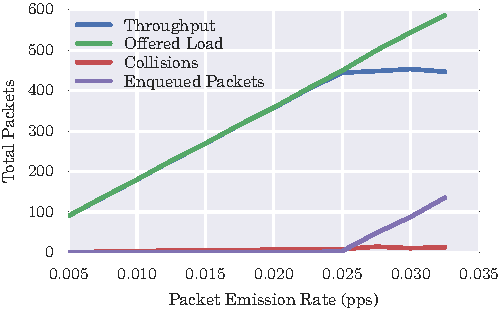
\includegraphics[width=\textwidth]{emission_throughput_performance_bella_static}
		\caption{Static}
		\label{fig:emission_throughput_performance_sum_bella_static}
	\end{subfigure}
	\begin{subfigure}[t]{0.5\textwidth}
		\centering
		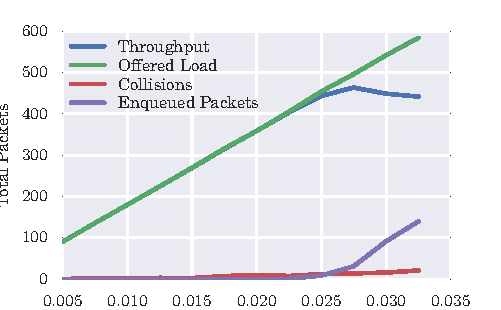
\includegraphics[width=\textwidth]{emission_throughput_performance_bella_all_mobile}
		\caption{All Mobile}
		\label{fig:emission_throughput_performance_sum_bella_all_mobile}
	\end{subfigure}  
	
	\begin{subfigure}[t]{0.5\textwidth}
		\centering
		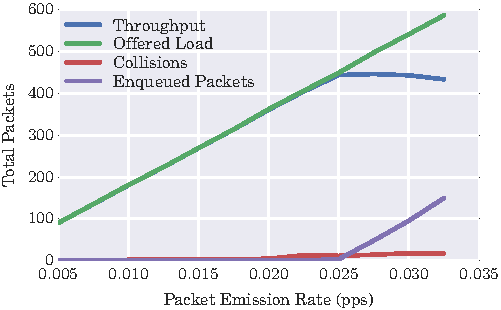
\includegraphics[width=\textwidth]{emission_throughput_performance_bella_allbut1_mobile}
		\caption{All-but-one Mobile}
		\label{fig:emission_throughput_performance_sum_bella_allbut1_mobile}
	\end{subfigure}  
	\begin{subfigure}[t]{0.5\textwidth}
		\centering
		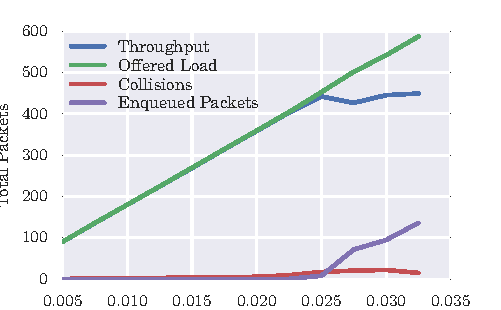
\includegraphics[width=\textwidth]{emission_throughput_performance_bella_single_mobile}
		\caption{Single Mobile}
		\label{fig:emission_throughput_performance_sum_bella_single_mobile}
	\end{subfigure}
	\caption{Throughput performance overview for all mobilities under varying emission rates}
	\label{fig:emission_all}
\end{figure}


\begin{figure}[tp!]
	\begin{subfigure}[t]{0.5\textwidth}
		\centering
		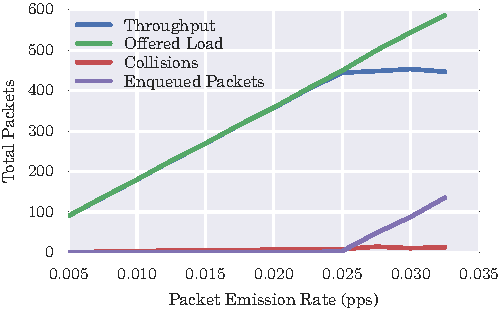
\includegraphics[width=\textwidth]{emission_throughput_performance_bella_static}
		\caption{Packet delivery}
		\label{fig:emission_throughput_performance_bella_static}
	\end{subfigure}
	%
	\begin{subfigure}[t]{0.5\textwidth}
		\centering
		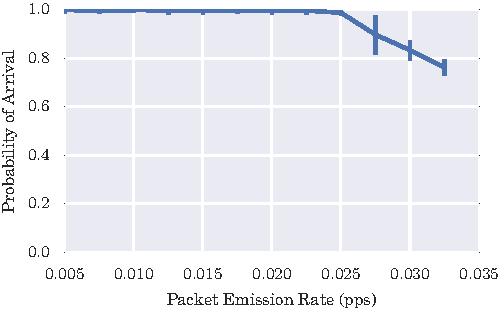
\includegraphics[width=\textwidth]{emission_prod_breakdown_bella_static}
		\caption{Probability of arrival}
		\label{fig:emission_prod_breakdown_bella_static}
	\end{subfigure}
	
	\begin{subfigure}[t]{0.5\textwidth}
		\centering
		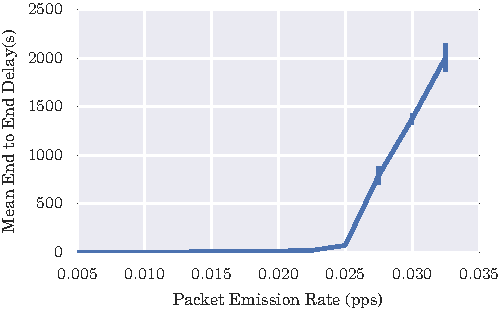
\includegraphics[width=\textwidth]{emission_delay_variation_bella_static}
		\caption{End-to-end delay}
		\label{fig:emission_delay_variation_bella_static}
	\end{subfigure}
	%
	\begin{subfigure}[t]{0.5\textwidth}
		\centering
		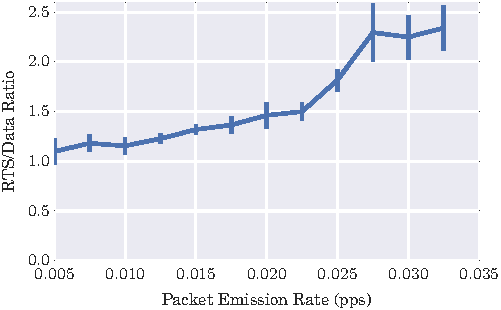
\includegraphics[width=\textwidth]{emission_rts_ratio_bella_static}
		\caption{RTS Ratios}
		\label{fig:emission_rts_ratio_bella_static}
	\end{subfigure}
	\caption{Network performance varying packet emission rates for the static case}
	\label{fig:emission_bella_static}
\end{figure}


\begin{figure}[bp!]
	\begin{subfigure}[t]{0.5\textwidth}
		\centering
		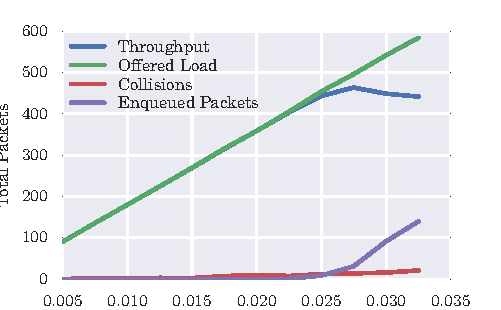
\includegraphics[width=\textwidth]{emission_throughput_performance_bella_all_mobile}
		\caption{Packet delivery}
		\label{fig:emission_throughput_performance_bella_all_mobile}
	\end{subfigure}
	%
	\begin{subfigure}[t]{0.5\textwidth}
		\centering
		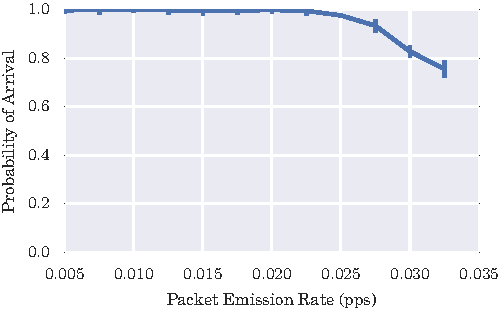
\includegraphics[width=\textwidth]{emission_prod_breakdown_bella_all_mobile}
		\caption{Probability of arrival}
		\label{fig:emission_prod_breakdown_bella_all_mobile}
	\end{subfigure}
	
	\begin{subfigure}[t]{0.5\textwidth}
		\centering
		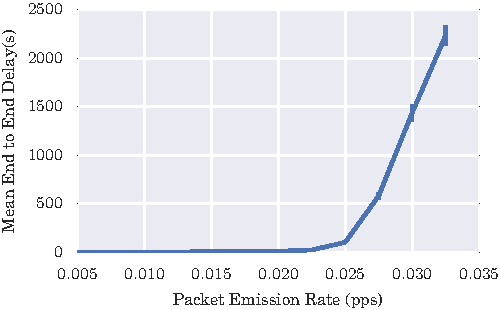
\includegraphics[width=\textwidth]{emission_delay_variation_bella_all_mobile}
		\caption{End-to-end delay}
		\label{fig:emission_delay_variation_bella_all_mobile}
	\end{subfigure}
	%
	\begin{subfigure}[t]{0.5\textwidth}
		\centering
		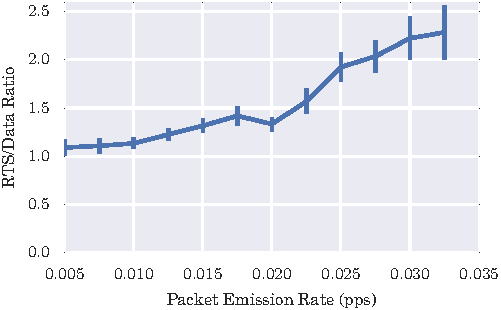
\includegraphics[width=\textwidth]{emission_rts_ratio_bella_all_mobile}
		\caption{RTS Ratios}
		\label{fig:emission_rts_ratio_bella_all_mobile}
	\end{subfigure}
	\caption{Network performance varying packet emission rates for the all mobile case}
	\label{fig:emission_bella_all_mobile}
\end{figure}


\begin{figure}[tp!]
	\begin{subfigure}[t]{0.5\textwidth}
		\centering
		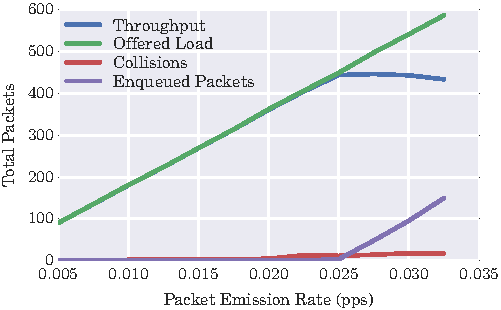
\includegraphics[width=\textwidth]{emission_throughput_performance_bella_allbut1_mobile}
		\caption{Packet delivery}
		\label{fig:emission_throughput_performance_bella_allbut1_mobile}
	\end{subfigure}
	%
	\begin{subfigure}[t]{0.5\textwidth}
		\centering
		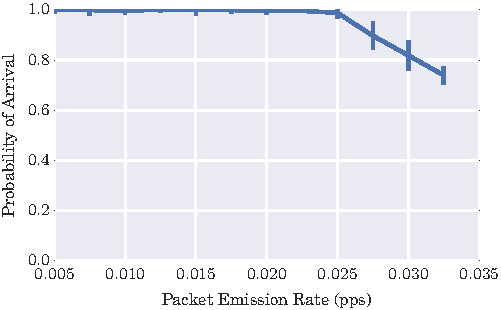
\includegraphics[width=\textwidth]{emission_prod_breakdown_bella_allbut1_mobile}
		\caption{Probability of arrival}
		\label{fig:emission_prod_breakdown_bella_allbut1_mobile}
	\end{subfigure}
	
	\begin{subfigure}[t]{0.5\textwidth}
		\centering
		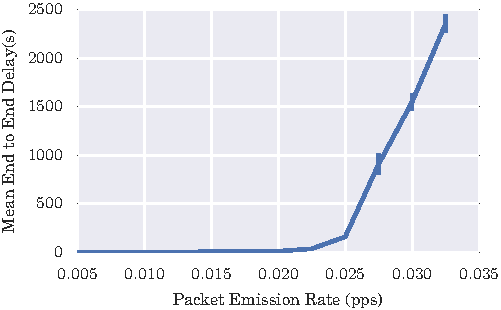
\includegraphics[width=\textwidth]{emission_delay_variation_bella_allbut1_mobile}
		\caption{End-to-end delay}
		\label{fig:emission_delay_variation_bella_allbut1_mobile}
	\end{subfigure}
	%
	\begin{subfigure}[t]{0.5\textwidth}
		\centering
		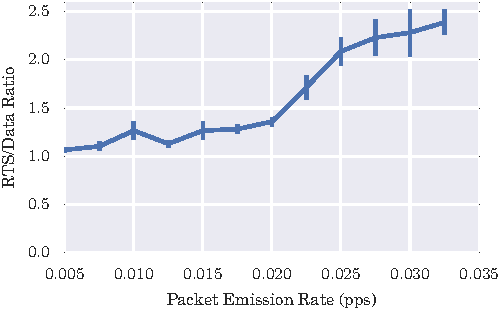
\includegraphics[width=\textwidth]{emission_rts_ratio_bella_allbut1_mobile}
		\caption{RTS Ratios}
		\label{fig:emission_rts_ratio_bella_allbut1_mobile}
	\end{subfigure}
	\caption{Network performance varying packet emission rates for the all-but-one mobile case}
	\label{fig:emission_bella_allbut1_mobile}
\end{figure}

\begin{figure}[bp!]
	\begin{subfigure}[t]{0.5\textwidth}
		\centering
		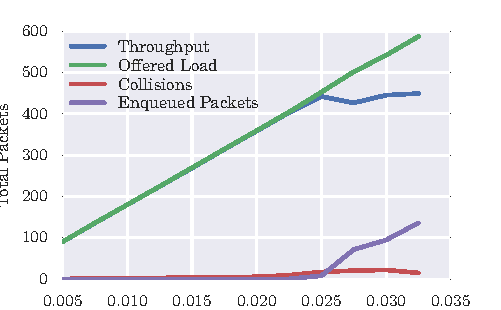
\includegraphics[width=\textwidth]{emission_throughput_performance_bella_single_mobile}
		\caption{Packet delivery}
		\label{fig:emission_throughput_performance_bella_single_mobile}
	\end{subfigure}
	%
	\begin{subfigure}[t]{0.5\textwidth}
		\centering
		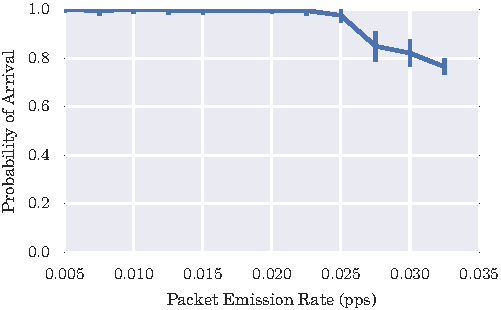
\includegraphics[width=\textwidth]{emission_prod_breakdown_bella_single_mobile}
		\caption{Probability of arrival}
		\label{fig:emission_prod_breakdown_bella_single_mobile}
	\end{subfigure}
	
	\begin{subfigure}[t]{0.5\textwidth}
		\centering
		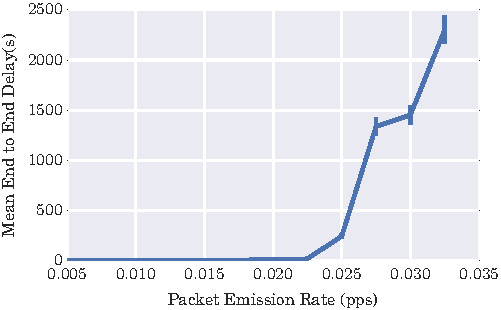
\includegraphics[width=\textwidth]{emission_delay_variation_bella_single_mobile}
		\caption{End-to-end delay}
		\label{fig:emission_delay_variation_bella_single_mobile}
	\end{subfigure}
	%
	\begin{subfigure}[t]{0.5\textwidth}
		\centering
		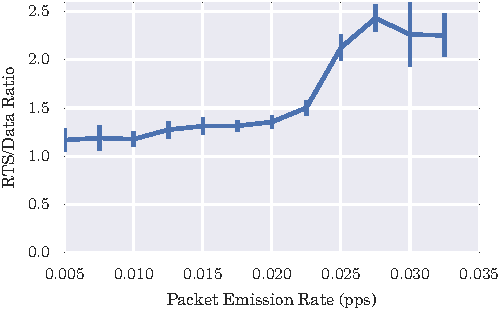
\includegraphics[width=\textwidth]{emission_rts_ratio_bella_single_mobile}
		\caption{RTS Ratios}
		\label{fig:emission_rts_ratio_bella_single_mobile}
	\end{subfigure}
	\caption{Network performance varying packet emission rates for the single mobile case}
	\label{fig:emission_bella_single_mobile}
\end{figure}

\clearpage

\subsection{Scale Factors in Physical Node Distribution}

In this section the effect of node-separation scaling on communications operation is characterised for comparison against \cite{Guo11}. 
This is particularly important considering the significant scale factor differences in terms of the speed of propagation in the medium, and the range of potential desired operation.

From~\autoref{tab:sysconstraints}, the operating transmission range of acoustic is $\approx 6$ times further than 802.11, indicating that a suitable operating environment will have an area $\approx \sqrt{6}$ times the area of the 802.11 case. Therefore, a reasonable experimental range would have an upper bound of performance around this scaling factor, where nodes are approximately 400$m$ apart. 

According to \citet{Xu2002}, \gls{rts}/\gls{cts} handshake functionality cannot operate well as interference protection at node separations beyond 0.56 times the transmission range\cite{Xu2002}.
In the case of marine acoustic transmission at the stated power output, above $1500m \times 0.56 = 840m$, handshake overheads should begin to dominate channel access.\todo{FIX CODE:redo these graphs with wider separations ~ 1000m}
This is due to reduced channel availability due to collisions, which are then due to a much longer potential contention period between nodes. 

A reasonable range around this is to scale from 100$m$ apart on average to $800m$, and from the previous section, a packet emission rate of $0.02pps$ (slightly below the $0.025pps$ saturation threshold) is used to explore this space.
The ``environment'' of the simulations is also scaled in accordance with the node scaling, based on an initial environmental ``water-box'' of $1km$ for the $100m$ node separation, i.e.\ the water-box is consistently ten times larger than the initial node separation.

In the case where all nodes remain static, increasing node separation does not significantly impact throughput, delay, delivery probability or \gls{rts} ratios until rising above 700$m$ (Fig.~\ref{fig:separation_bella_static}), nearly double our initial estimate of where an appropriate separation zone would be.

The other mobility cases tell a very different story; as can be seen in~\autoref{fig:separation_throughput_performance_sum_bella_single_mobile}, where adding a single mobile node to the network induces a saturation-style response at 500$m$, and this drops further in~\autoref{fig:separation_throughput_performance_sum_bella_allbut1_mobile} and~\autoref{fig:separation_throughput_performance_sum_bella_all_mobile}, reducing the separation of saturation at this emission rate to just 300$m$.

Another aspect of these results to highlight is that the Offered Load presented to the network \emph{increases} beyond the collapse of the throughput curve. 
This indicates that there is a subtly different saturation behaviour with respect to separation than the simple congestion argument with respect to packet emission rate; packets are simply taking too long to cross the increasingly sparse network and in-transit packet routes are logically disconnected and require retransmission.



\subsection{Combined Scale Factor Analysis}
\begin{figure}[h]
	\begin{subfigure}[t]{0.5\textwidth}
		\centering
		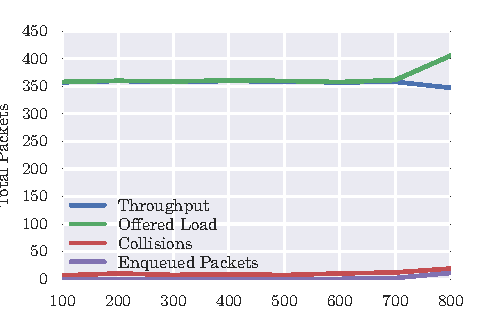
\includegraphics[width=\textwidth]{separation_throughput_performance_bella_static}
		\caption{Static}
		\label{fig:separation_throughput_performance_sum_bella_static}
	\end{subfigure}
	\begin{subfigure}[t]{0.5\textwidth}
		\centering
		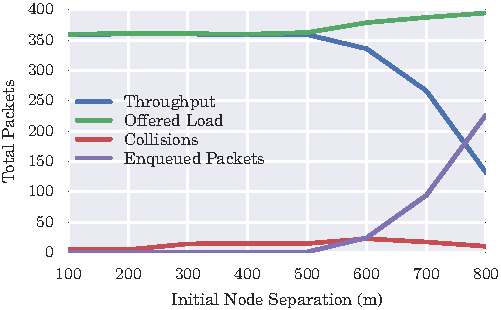
\includegraphics[width=\textwidth]{separation_throughput_performance_bella_single_mobile}
		\caption{Single Mobile}
		\label{fig:separation_throughput_performance_sum_bella_single_mobile}
	\end{subfigure}
	
	\begin{subfigure}[t]{0.5\textwidth}
		\centering
		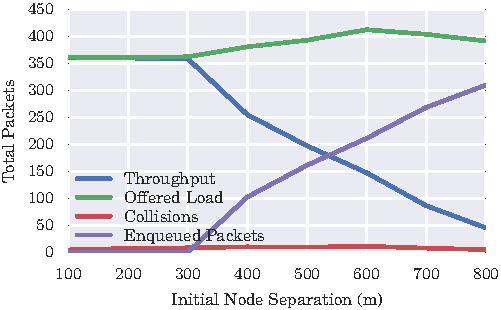
\includegraphics[width=\textwidth]{separation_throughput_performance_bella_allbut1_mobile}
		\caption{All-but-one Mobile}
		\label{fig:separation_throughput_performance_sum_bella_allbut1_mobile}
	\end{subfigure}  
	\begin{subfigure}[t]{0.5\textwidth}
		\centering
		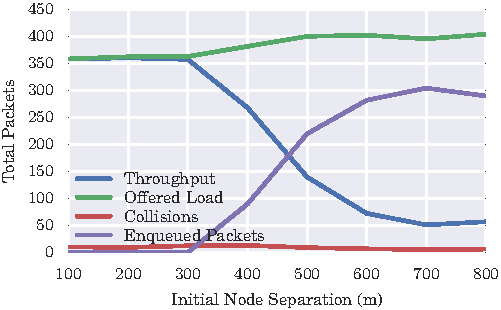
\includegraphics[width=\textwidth]{separation_throughput_performance_bella_all_mobile}
		\caption{All Mobile}
		\label{fig:separation_throughput_performance_sum_bella_all_mobile}
	\end{subfigure}  
	\caption{Throughput performance overview for all mobilities under varying separation}
	\label{fig:separation_all}
\end{figure}

% These figures should be colocated
\begin{figure}[tp!]
	\begin{subfigure}[t]{0.5\textwidth}
		\centering
		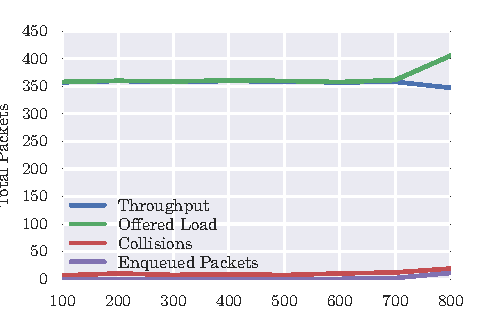
\includegraphics[width=\textwidth]{separation_throughput_performance_bella_static}
		\caption{Packet delivery}
		\label{fig:separation_throughput_performance_bella_static}
	\end{subfigure}
	%
	\begin{subfigure}[t]{0.5\textwidth}
		\centering
		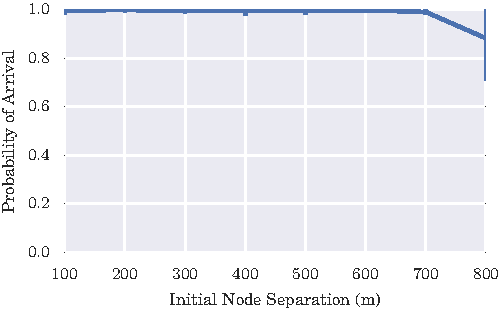
\includegraphics[width=\textwidth]{separation_prod_breakdown_bella_static}
		\caption{Probability of arrival}
		\label{fig:separation_prod_breakdown_bella_static}
	\end{subfigure}
	
	\begin{subfigure}[t]{0.5\textwidth}
		\centering
		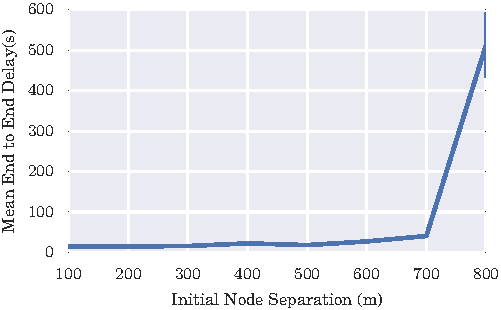
\includegraphics[width=\textwidth]{separation_delay_variation_bella_static}
		\caption{End-to-end delay}
		\label{fig:separation_delay_variation_bella_static}
	\end{subfigure}
	%
	\begin{subfigure}[t]{0.5\textwidth}
		\centering
		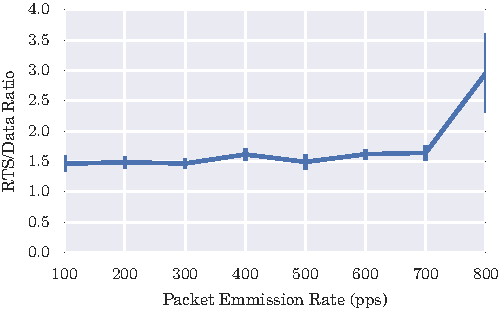
\includegraphics[width=\textwidth]{separation_rts_ratio_bella_static}
		\caption{RTS Ratios}
		\label{fig:separation_rts_ratio_bella_static}
	\end{subfigure}
	\caption{Network performance varying node separation for the static case}
	\label{fig:separation_bella_static}
\end{figure}


\begin{figure}[bp!]
	\begin{subfigure}[t]{0.5\textwidth}
		\centering
		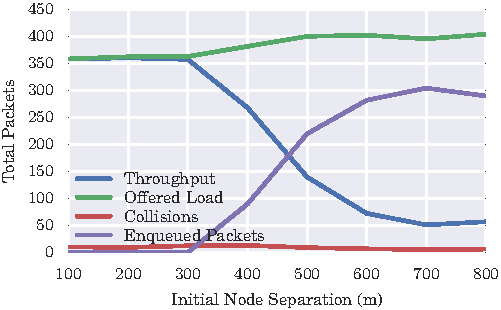
\includegraphics[width=\textwidth]{separation_throughput_performance_bella_all_mobile}
		\caption{Packet delivery}
		\label{fig:separation_throughput_performance_bella_all_mobile}
	\end{subfigure}
	%
	\begin{subfigure}[t]{0.5\textwidth}
		\centering
		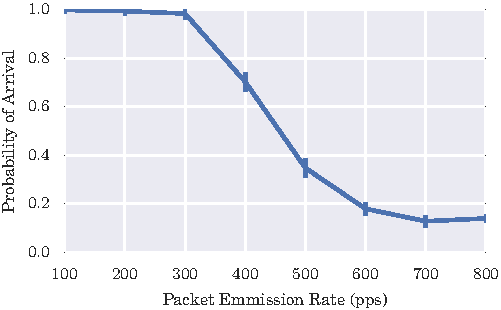
\includegraphics[width=\textwidth]{separation_prod_breakdown_bella_all_mobile}
		\caption{Probability of arrival}
		\label{fig:separation_prod_breakdown_bella_all_mobile}
	\end{subfigure}
	
	\begin{subfigure}[t]{0.5\textwidth}
		\centering
		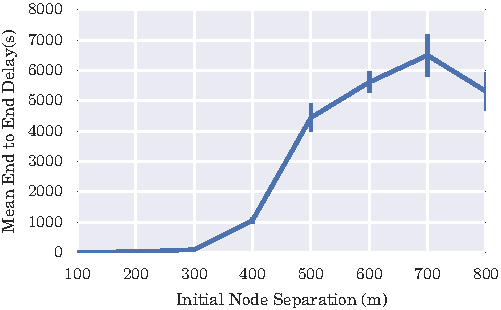
\includegraphics[width=\textwidth]{separation_delay_variation_bella_all_mobile}
		\caption{End-to-end delay}
		\label{fig:separation_delay_variation_bella_all_mobile}
	\end{subfigure}
	%
	\begin{subfigure}[t]{0.5\textwidth}
		\centering
		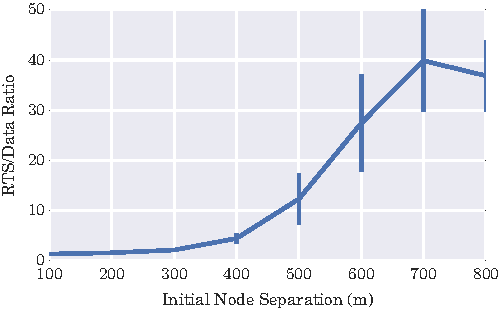
\includegraphics[width=\textwidth]{separation_rts_ratio_bella_all_mobile}
		\caption{RTS Ratios}
		\label{fig:separation_rts_ratio_bella_all_mobile}
	\end{subfigure}
	\caption{Network performance varying node separation for the all mobile case}
	\label{fig:separation_bella_all_mobile}
\end{figure}


\begin{figure}[tp!]
	\begin{subfigure}[t]{0.5\textwidth}
		\centering
		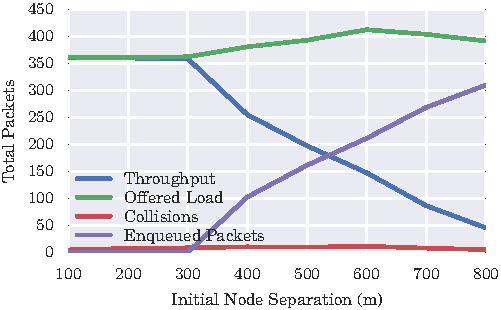
\includegraphics[width=\textwidth]{separation_throughput_performance_bella_allbut1_mobile}
		\caption{Packet delivery}
		\label{fig:separation_throughput_performance_bella_allbut1_mobile}
	\end{subfigure}
	%
	\begin{subfigure}[t]{0.5\textwidth}
		\centering
		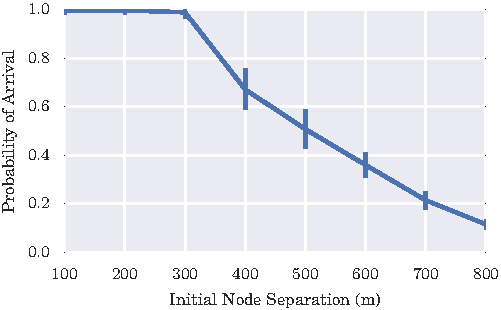
\includegraphics[width=\textwidth]{separation_prod_breakdown_bella_allbut1_mobile}
		\caption{Probability of arrival}
		\label{fig:separation_prod_breakdown_bella_allbut1_mobile}
	\end{subfigure}
	
	\begin{subfigure}[t]{0.5\textwidth}
		\centering
		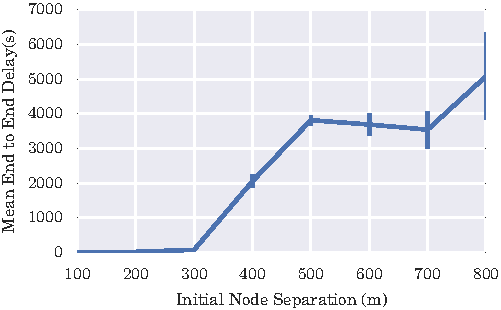
\includegraphics[width=\textwidth]{separation_delay_variation_bella_allbut1_mobile}
		\caption{End-to-end delay}
		\label{fig:separation_delay_variation_bella_allbut1_mobile}
	\end{subfigure}
	%
	\begin{subfigure}[t]{0.5\textwidth}
		\centering
		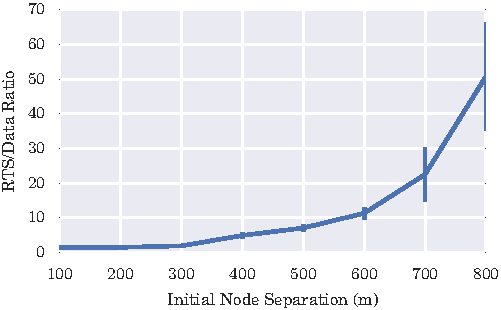
\includegraphics[width=\textwidth]{separation_rts_ratio_bella_allbut1_mobile}
		\caption{RTS Ratios}
		\label{fig:separation_rts_ratio_bella_allbut1_mobile}
	\end{subfigure}
	\caption{Network performance varying node separation for the all-but-one mobile case}
	\label{fig:separation_bella_allbut1_mobile}
\end{figure}

\begin{figure}[bp!]
	\begin{subfigure}[t]{0.5\textwidth}
		\centering
		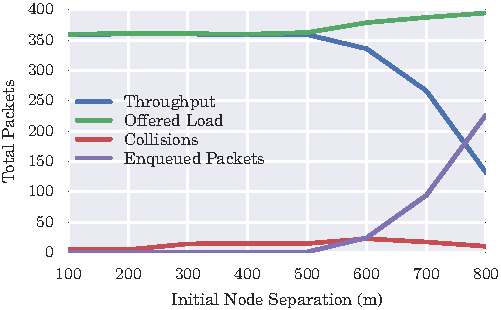
\includegraphics[width=\textwidth]{separation_throughput_performance_bella_single_mobile}
		\caption{Packet delivery}
		\label{fig:separation_throughput_performance_bella_single_mobile}
	\end{subfigure}
	%
	\begin{subfigure}[t]{0.5\textwidth}
		\centering
		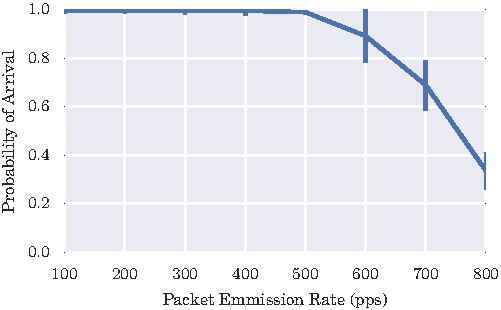
\includegraphics[width=\textwidth]{separation_prod_breakdown_bella_single_mobile}
		\caption{Probability of arrival}
		\label{fig:separation_prod_breakdown_bella_single_mobile}
	\end{subfigure}
	
	\begin{subfigure}[t]{0.5\textwidth}
		\centering
		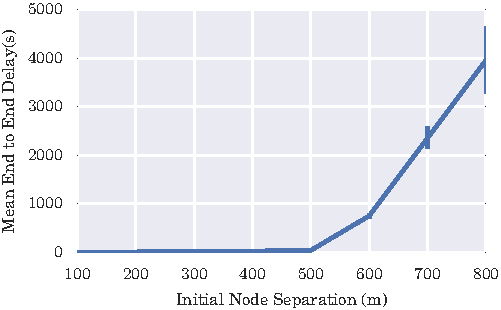
\includegraphics[width=\textwidth]{separation_delay_variation_bella_single_mobile}
		\caption{End-to-end delay}
		\label{fig:separation_delay_variation_bella_single_mobile}
	\end{subfigure}
	%
	\begin{subfigure}[t]{0.5\textwidth}
		\centering
		\includegraphics[width=\textwidth]{separation_rts_ratio_bella_single_mobile}
		\caption{RTS Ratios}
		\label{fig:separation_rts_ratio_bella_single_mobile}
	\end{subfigure}
	\caption{Network performance varying node separation for the single mobile case}
	\label{fig:separation_bella_single_mobile}
\end{figure}


% scripts.publication_scripts.test_Thesis_lazy.ThesisLazyDiagrams#test_PacketStatsGraphs
\begin{table}[h]
	\caption{Tabular view of data from~\autoref{fig:separation_bella_single_mobile}, including ideal propagation time} \label{tab:separation_bella_single_mobile}
	\begin{center}
		\hyphenpenalty 10000
		\begin{tabular}{
            *{2}{@{\hspace{1em}}r@{\hspace{1em}}}
            *{3}{@{\hspace{1em}}p{0.1\textwidth} @{\hspace{1em}}}  }
\toprule
 Initial Node Separation (m) &  Delay(s) &  Probability of Arrival &  RTS/Data Ratio &  Ideal Delivery Time(s) \\
\midrule
                         100 &   10.3551 &                  0.9977 &          1.3546 &                  1.0314 \\
                         200 &   11.1631 &                  0.9973 &          1.3322 &                  1.1029 \\
                         300 &   24.2225 &                  0.9983 &          1.5650 &                  1.1743 \\
                         400 &   29.4864 &                  0.9965 &          1.6210 &                  1.2457 \\
                         500 &   41.7093 &                  0.9904 &          1.8331 &                  1.3171 \\
                         600 &  753.4040 &                  0.8922 &          2.8038 &                  1.3886 \\
                         700 & 2360.0826 &                  0.6899 &          4.3889 &                  1.4600 \\
                         800 & 3963.9830 &                  0.3360 &         12.7323 &                  1.5314 \\
\bottomrule
\end{tabular}

	\end{center}
\end{table}


\clearpage





Its clear from the previous results that the relationship between emission rates, separations and mobilities is tightly coupled and not totally clear cut. 
To arrive at a more optimal operating region, a coupled analysis is performed across both emission rate and initial separation distance.

Given what has been discussed so far; it's clear that in identifying an appropriate operating region, it is important to not only ensure throughput, but that that throughput is timely.
For instance, in~\autoref{fig:separation_bella_single_mobile} (tabulated in~\autoref{tab:separation_bella_single_mobile}), a small increase in separation beyond the apparent throughput-peak at 500$m$ to 600$m$, which constitutes an increased ideal marine acoustic ``time of flight'' between nodes by 0.02$s$, increases the average actual delay by 1800\%. 

To capture these performance requirements, the feature scaled product of Throughput and Delay is taken and plotted against rate and separation in~\autoref{fig:2d_normed_product}.\todo[inline]{FIX: This does NOT make for easy comparison between graphs as the scaling is different for each mobility, but I need to think about how to fairly solve this}

\begin{equation}
V = |S] \times (1 - |D|)
\label{eq:normed_product}
\end{equation}

For each scenario, the observed Throughput across the network ($S$ in bytes) is normalised across all observations (i.e.\ each combination of Node Separation and Emission Rate), as is average end-to-end Delay ($D$). The normalised delay is inverted ($1-|D|$) and the product of this and the normalised throughput is used as the basis of a two-dimensional linear interpolation shown in \autoref{fig:2d_normed_product}.




\begin{figure}[h]
	\begin{subfigure}[t]{0.5\textwidth}
		\centering
		\includegraphics[width=\textwidth]{2d_normed_product_bella_static}
		\caption{Static}
		\label{fig:2d_normed_product_bella_static}
	\end{subfigure}
	\begin{subfigure}[t]{0.5\textwidth}
		\centering
		\includegraphics[width=\textwidth]{2d_normed_product_bella_single_mobile}
		\caption{Single Mobile}
		\label{fig:2d_normed_product_bella_single_mobile}
	\end{subfigure}
	
	\begin{subfigure}[t]{0.5\textwidth}
		\centering
		\includegraphics[width=\textwidth]{2d_normed_product_bella_allbut1_mobile}
		\caption{All-but-one Mobile}
		\label{fig:2d_normed_product_bella_allbut1_mobile}
	\end{subfigure}
	\begin{subfigure}[t]{0.5\textwidth}
		\centering
		\includegraphics[width=\textwidth]{2d_normed_product_bella_all_mobile}
		\caption{All Mobile}
		\label{fig:2d_normed_product_bella_all_mobile}
	\end{subfigure}
	\caption{Normalised Throughput-Delay Product for all mobilities under varying separation and emission rate}
	\label{fig:2d_normed_product}
\end{figure}


\subsection{Summary}

An appropriate safe operating zone for marine communications has been established by investigating the impact of variations of the communications rate and physical distribution across the mobility scenarios.

These findings can be summaries as that when the separation is increased, the emission rate at which the network becomes saturated decreases, reducing overall throughput. 
This throughput degradation is tightly coupled with the mobility, as increasing mobility leads to increasing delays as routes are constantly broken, re-advertised and re-established. 
For instance, where all nodes are static, significant drops in throughput are not seen until node separation approaches $800m$, nearly double the initial estimate. 
However, when all nodes are randomly walking the saturation point collapses from $0.025pps$ at $300m$ to $0.015pps$ at $400m$.\todo[inline]{FIX:Double Check These Saturation Points Before Release}
These results indicate that a good area to continue operating in for a range of node separations is at $0.015pps$, and that a reasonable position scaling is from $100m$ to $300m$, beyond which communication becomes increasingly unstable, especially in terms of end-to-end delay.
These results are similar to related simulation work \cite{Miquel2008,Diamant2010,Noh2012}, and is to be expected in such a sparse, noisy, and contentious environment.
It should be noted that these rates are not what would be expected in a single-node/single-operator environment that most current \gls{auv} operations inhabit, as without any channel contention and mixed-delay effects, data-rates many times higher than this would be expected.
However, few practical experiments have been performed that are suitable for direct comparison, as this context relies on multiple available nodes in a dynamic \gls{manet} topology with differential mobility.


\todo{ADD:expand this section to include discussion and results of single mobility models}
The results from \autoref{fig:2d_normed_product_bella_single_mobile} and \autoref{fig:2d_normed_product_bella_allbut1_mobile} show that the single-node differential mobility models don't capture the reality of the network in the proposed port-protection context.
The reason for this is that in these single-differential mobility combinations, the node targeted for misbehaviour ($n_1$) will already be behaving differently compared to the rest of the network regardless of the misbehaviour.
A future extension to this work could be to look at differential ratios of static/mobile nodes in alternative scenarios, such as in data-muling applications or \gls{wsn}.

\section{Operation of \glspl{tmf} in \glspl{uan}}

We are primarily concerned with the direct trust relationship between $n_0$ and $n_1$, i.e. $n_0$'s assessment of the trustworthiness of $n_1$, or $T_{1,0}$.

\citet{Guo11} introduce a range of misbehaviours, including modification of the packet loss rate of routing nodes and limiting throughput on a per-link basis as well as a selection of combined misbehaviours. 
\todo{FIX:Link back to intro/bg misbehaviour dicussion}
Given that the established links are already heavily constrained, such attacks would severely impact the general performance of the network beyond the scope of simple selfishness.
These direct malicious behaviours effectively trigger saturation collapses in operating regions of the network that should be stable.

Therefore, two more subtle misbehaviours to investigate are; 
\begin{enumerate}
	\item \acrfull{mpc}, where $n_1$ increases its transmit and forwarding power by 20\% for all nodes \emph{except} communications from $n_0$ in order to make $n_0$ appear to be selfishly conserving energy to the rest of the team, while $n_1$ itself appears to be performing very well.
	\item \acrfull{sts}, where $n_1$ preferentially communicates, forwards and advertises to nodes that are physically close to it in effort to reduce its own power consumption.
\end{enumerate}


\section{Simulation Results and Discussion}\label{sec:trustresultsanddiscussion}

Having established a safe operating range for comparison at $300m$ average separation and an emission rate of $0.015pps$, each of the three selected behaviours (Fair, \gls{mpc}, \gls{sts}) are performed in both the static and mobile scenarios. 
We select a trust assessment period of 10 mins for a five hour mission to scale in comparison to relative bitrates experienced ($1Mbps$ vs $\approx15bps$).

The six metrics used for grey assessment are; transmitted and received throughput and power, delay, and \gls{plr} as calculated by aborted and unacknowledged, transmissions.
Compared to \cite{Guo11}, this metric set lacks a data rate quantity as the network is not dynamically adjusting bandwidth.
In context of \gls{grc} generation \eqref{eq:grc}, the best sequence $g$ was selected using the lowest \gls{plr}, delay, and powers, and the highest throughputs, and the worst sequence, $b$ the inverse of these metrics, reflecting the observations made in \autoref{sec:trust_in_marine}.

The particular factors under discussion are the relative performance of \gls{mtfm} against \gls{otmf} and Beta with respect to statistical stability across mobilities and in responsiveness to changing network behaviour. 
We establish a similar result set by initially tracking the resultant trust values established by \gls{mtfm} in the pair of mobility scenarios, shown in Fig.~\ref{fig:trust_mobility}.
We are also concerned with the opinions of $n_1$ provided to $n_0$ by other nodes, where $[T_{2,1},T_{3,1}]$ and $[T_{4,1},T_{5,1}]$ denote the sets of recommendation and indirect trust assessment respectively.

We also include aggregate assessments; $T_{N,1}^\text{Avg}$, the unweighted mean of direct trust assessments of $n_1$ from all nodes and $T_{0,1}^\text{MTFM}$, the final \gls{mtfm} trust assessment value based on both network topology with respect to $n_0$ and whitenization from \eqref{eq:whitenization}.

The variability in assessment is coupled to mobility; in the static case (Fig.~\ref{fig:trust_static}), the nodes exhibit relatively consistent distributions.
In the full mobility case, shown in Fig.~\ref{fig:trust_all_mobile}, this subjective variability is greatly increased. 
As the topology is highly dynamic, delays due to re-establishing routes can be very large, perturbing the trust value.
The $T_{0,1}^\text{MTFM}$ displays a significantly reduced variation than those of the individual subjective observations in all cases, even when compared to the unweighted average, $T_{N,1}^\text{Avg}$.
This demonstrates $T_{MTFM}$'s value as an aggregating trust assessment in such sparse and noisy environments.
Further, in Fig.~\ref{fig:trust_all_mobile_mal} a much higher variability in assessment is observed in $T_{0,1}$, correctly indicating that there is something wrong with the relationship between $n_0$ and $n_1$.

\begin{figure}[h]
	\centering
	\begin{subfigure}{0.5\textwidth}
		\caption{Fair Static}
		\includegraphics[width=\linewidth]{trust_bella_static_fair} 
		\label{fig:trust_static}
	\end{subfigure}%
	\begin{subfigure}{0.5\textwidth}
		\caption{Fair Mobile}
		\includegraphics[width=\linewidth]{trust_bella_all_mobile_fair}  
		\label{fig:trust_all_mobile}
	\end{subfigure}%
	
	\begin{subfigure}{0.5\textwidth}
		\caption{Malicious (MPC) Static}
		\includegraphics[width=\linewidth]{trust_bella_static_malicious} 
		\label{fig:trust_static_mal}
	\end{subfigure}%
	\begin{subfigure}{0.5\textwidth}
		\caption{Malicious (MPC) Mobile}
		\includegraphics[width=\linewidth]{trust_bella_all_mobile_malicious}  
		\label{fig:trust_all_mobile_mal}
	\end{subfigure}%
	
	\begin{subfigure}{0.5\textwidth}
		\caption{Selfish (STS) Static}
		\includegraphics[width=\linewidth]{trust_bella_static_selfish}
		\label{fig:trust_static_sel}
	\end{subfigure}%
	\begin{subfigure}{0.5\textwidth}
		\caption{Selfish (STS) Mobile}
		\includegraphics[width=\linewidth]{trust_bella_all_mobile_selfish}  \label{fig:trust_all_mobile_sel}
	\end{subfigure}%
	
	\caption{\gls{mtfm} Trust assessments of $n_1$ ($T_{X,1}$), showing Direct, Recommender and Indirect relationships, and derived aggregates} 
	\label{fig:trust_mobility}
\end{figure}
%

\subsection{Comparison between \gls{mtfm}, Hermes and \gls{otmf}}
As per \citet{Guo11}, ``fair'' scenarios were also performed with no malicious behaviour, applying \gls{otmf} and Hermes assessment as well as \gls{mtfm}, providing like-for-like comparison of assessment.

\begin{figure*}[t]
	\centering
	\begin{tabular}{cc}
		\multirow{2}{*}{
			\begin{subfigure}{0.45\textwidth}	
				\includegraphics[width=\linewidth]{trust_beta_otmf_fair}
				\caption{Fair Scenario}
				\label{fig:all_mobile_fair_beta}
			\end{subfigure}
		}&
		\begin{subfigure}{0.45\textwidth}
			\includegraphics[width=\linewidth]{trust_beta_otmf_malicious} 
			\caption{Malicious Power Control (MPC) Scenario}
			\label{fig:all_mobile_badmouthing_beta}
		\end{subfigure} \\
		&
		\begin{subfigure}{0.45\textwidth}	
			\includegraphics[width=\linewidth]{trust_beta_otmf_selfish} 
			\caption{Selfish Target Selection (STS) Scenario}
			\label{fig:all_mobile_selfish_beta}
		\end{subfigure}
	\end{tabular}
	\caption{$T_{0,1}$ for Hermes, \gls{otmf} and \gls{mtfm} assessment values for fair and malicious behaviours in the fully mobile scenario}
	\label{fig:otmf_beta_comparison}
\end{figure*}
%
\begin{figure}
	\centering
	\includegraphics[width=0.9\textwidth]{trust_beta_otmf_mtfm_boxes}
	\caption{Alternative Visualisation of \gls{tmf} performance comparison across Fair, \gls{mpc}, and \gls{sts} scenarios}
	\label{fig:otmf_beta_comparison_boxes}
\end{figure}
The use of \gls{fbr} and a \gls{csmaca} \gls{mac} scheme from AUVNetSim~\cite{Miquel2008} in our simulation mitigates a significant number of packet losses through collision avoidance and contention handling, leading to the situation that the only genuinely lost packets occur when a node moves completely out of range of any other node and time out occurs in route discovery rather than transmission (See \autoref{sec:manet_routing}).
As such, confirmed packet losses are relatively rare and in a delaying network like this, it is difficult to set a differentiating time out between packets that are in the network but queued, and packets that are actually ``lost''.

The single metric \glspl{tmf} used in conventional \gls{manet}s require regular and constant input to shape and adjust their evaluations, which for a network with significant and irregular delays such as this, is not practical.
This renders \gls{otmf} and Hermes assessment at best uninformative and at worst misleading; consistently providing nodes a high trust assessment as they have very little information to extract trust from. 

\autoref{fig:otmf_beta_comparison} shows a comparison between the unweighted response of \gls{mtfm} compared to \gls{otmf} and Hermes assessment functions on the same data for the fair, malicious and selfish behaviours respectively.
This time-series perspective demonstrates how noisy and variable the assessments from all \glspl{tmf} in this environment.
For clarity, \autoref{fig:otmf_beta_comparison_boxes} displays a compressed-time perspective, showing the overall trend and sensitivity of the different frameworks in the same scenarios as shown in \autoref{fig:otmf_beta_comparison}.
It is important to note a distinction between the expectations of \gls{mtfm} compared to other \glspl{tmf}; \gls{mtfm} is primarily concerned with the identification of differences in the behaviours of nodes in a network, and is relative rather than absolute.
That is to say that under \gls{mtfm}, nodes are compared against the worst current performances across metrics of other observed nodes and graded against them, rather than the absolute (objective) approach taken by many \glspl{tmf}.

In the case of the \gls{mpc}
In these cases, particularly since the methods of attack were not directly related to \gls{plr}, \gls{otmf} and Hermes have not registered significant activity in either misbehaviour when compared to the fair scenario.
The difference between the \gls{mtfm} trust assessments under ``fair'' and ``malicious'' behaviour is lowered by $\approx 10\%$ in both cases, in terms of the mean values returned.
At run time, similar results could be attained by an \gls{ewma}.

On their own, neither \gls{otmf}, Hermes, or unbiased \gls{mtfm} appear to be effective in detecting or identifying malicious behaviour in this environment, in fact \gls{otmf} and Hermes don't appear to differentiate between fair and selfish scenarios at all.



\subsection{Metric Vector Weighting}\label{sec:metric_weighting}
%

A sequence of vectors that preferentially weight each metric in \eqref{eq:metric_weighting} to each of the three simulation runs.
For a metric weight vector $H$, where the metric $m_j$ is emphasised as being twice as important as the other metrics, forming an initial weighting vector $H'=[h_i\dots h_M]$ such that $h_i = 1 \forall i \ne j; h_j=2$.
That vector $H'$ is normalised such that $\sum H = 1$ by $H= \frac{H'}{\sum H'}$.
Using this process the primary aspects of an attack can be extracted and highlighted by comparing against the deviation from the ``fair'' result set. 

\begin{figure}[h]
	\centering
	\begin{subfigure}{0.45\textwidth}
		\includegraphics[width=\linewidth]{trust_bella_all_mobile_emph_ADelay_BadMouthingPowerControl} 
		\caption{$\text{Delay}$ Emphasised}
		\label{fig:all_mobile_badmouthing_delay}
	\end{subfigure}
	\begin{subfigure}{0.45\textwidth}
		\includegraphics[width=\linewidth]{trust_bella_all_mobile_emph_PLR_BadMouthingPowerControl} 
		\caption{$PLR$ Emphasised}
		\label{fig:all_mobile_badmouthing_plr}
	\end{subfigure}
	
	\begin{subfigure}{0.45\textwidth}
		\includegraphics[width=\linewidth]{trust_bella_all_mobile_emph_ARXP_BadMouthingPowerControl} 
		\caption{Received Power ($P_{RX}$) Emphasised}
		\label{fig:all_mobile_badmouthing_rxp}
	\end{subfigure}	
	\begin{subfigure}{0.45\textwidth}
		\includegraphics[width=\linewidth]{trust_bella_all_mobile_emph_ATXP_BadMouthingPowerControl} 
		\caption{Transmit Power ($P_{TX}$) Emphasised}
		\label{fig:all_mobile_badmouthing_txp}
	\end{subfigure}
	
	\begin{subfigure}{0.45\textwidth}
		\includegraphics[width=\linewidth]{trust_bella_all_mobile_emph_RXThroughput_BadMouthingPowerControl} 
		\caption{Throughput ($S$) Emphasised}
		\label{fig:all_mobile_badmouthing_rxthroughput}
	\end{subfigure}
	\begin{subfigure}{0.45\textwidth}
		\includegraphics[width=\linewidth]{trust_bella_all_mobile_emph_TXThroughput_BadMouthingPowerControl} 
		\caption{Offered Load ($G$) Emphasised}
		\label{fig:all_mobile_badmouthing_txthroughput}
	\end{subfigure}
	\caption{$T_{1,0}^\text{MTFM}$ in the All Mobile case for the Malicious Power Control behaviour, including dashed $\pm\sigma$ envelope about the fair scenario}
	\label{fig:all_mobile_badmouthing}
\end{figure}
%
\begin{figure}[h]
	\centering
	\begin{subfigure}{0.45\textwidth}	
		\includegraphics[width=\linewidth]{trust_bella_all_mobile_emph_ADelay_SelfishTargetSelection} 
		\caption{$Delay$ Emphasised}
		\label{fig:all_mobile_selfish_delay}
	\end{subfigure}
	\begin{subfigure}{0.45\textwidth}	
		\includegraphics[width=\linewidth]{trust_bella_all_mobile_emph_PLR_SelfishTargetSelection}
		\caption{$PLR$ Emphasised}
		\label{fig:all_mobile_selfish_plr}
	\end{subfigure}
	
	\begin{subfigure}{0.45\textwidth}	
		\includegraphics[width=\linewidth]{trust_bella_all_mobile_emph_ARXP_SelfishTargetSelection}
		\caption{Received Power ($P_{RX}$) Emphasised}
		\label{fig:all_mobile_selfish_rxp}
	\end{subfigure}
	\begin{subfigure}{0.45\textwidth}
		\includegraphics[width=\linewidth]{trust_bella_all_mobile_emph_ATXP_SelfishTargetSelection}
		\caption{Transmit Power ($P_{TX}$) Emphasised}
		\label{fig:all_mobile_selfish_txp}
	\end{subfigure}
	
	\begin{subfigure}{0.45\textwidth}
		\includegraphics[width=\linewidth]{trust_bella_all_mobile_emph_RXThroughput_SelfishTargetSelection} 
		\caption{Throughput ($S$) Emphasised}
		\label{fig:all_mobile_selfish_rxthroughput}
	\end{subfigure}
	\begin{subfigure}{0.45\textwidth}
		\includegraphics[width=\linewidth]{trust_bella_all_mobile_emph_TXThroughput_SelfishTargetSelection} 
		\caption{Offered Load ($G$) Emphasised}
		\label{fig:all_mobile_selfish_txthroughput}
	\end{subfigure}
	\caption{$T_{1,0}^\text{MTFM}$ in the All Mobile case for the Selfish Target Selection behaviour, including dashed $\pm\sigma$ envelope about the fair scenario}
	\label{fig:all_mobile_selfish}
\end{figure}


Fig.~\ref{fig:all_mobile_badmouthing} shows that the malicious node is consistently outside the $\pm\sigma$ (one standard deviation above and below the mean) envelope of the fair scenario it's being compared to.
This is particularly true for \gls{plr}, with smaller impacts on delay, received power and offered load. 
This weighted delta in received throughput is minimal to insignificant compared to the width of the detection envelope, occasionally breaching the envelope for a short period. 

In the selfish case (Fig.~\ref{fig:all_mobile_selfish}) a much lower weighted delta in \gls{plr} and delay is observed, with greatly increased impact on transmission power.
In comparison to \cite{Guo11}, these results are qualitatively similar, however here the differences between the fair case and the misbehaviours are less clear than in the comparable terrestrial space.
\citet{Guo11} show similar types of behaviour but report a weighted delta from $\approx$ 0.4 to $\approx$ 0.9 across the simulation period, compared to our maximum delta in $P_{TX}$ in selfish behaviour (Fig.~\ref{fig:all_mobile_selfish_txp}) of $\approx$ 0.3 for an inconsistent interval.

\subsection{Weight Significance Analysis for Behaviour Classification}

For a more quantitative assessment of the viability of multi-metric trust assessment methods, taking the qualitative analysis above and apply a Random Forest regression \cite{Breiman2001} to assess the relative importance of the selected metrics on relative detectability of malicious behaviour. 
Random Forest accomplishes this by generating a large number of random regression trees and prunes these trees to fit incoming data.
The target function for this regression was the area between the target behaviours weighted $T_{MTFM}$ curve and the $\pm\sigma$ envelope of the base behaviour as shaded in Figs.~\ref{fig:all_mobile_badmouthing} and~\ref{fig:all_mobile_selfish}.
From this training process, the relative importance of each input feature (metric) can be inferred in terms of how good it is to differentiate between the fair case and a given misbehaviour.
Additionally a cross correlation analysis is performed to establish the correlations between given metric weighting emphasis and the output of the target function.
Our intention is to establish the metrics that not only differentiate both misbehaviours from the fair case, but also what metrics differentiate the two misbehaviours from each other.

Applying this target regression to 729 different metric weight vector emphasis combinations reveals that each of the three combinations (i.e.\ comparing fair to misbehaviours, and comparing the misbehaviours) present distinct patterns of significance in three primary metrics; received throughput, transmitted power, and PLR, with delay, received power and transmitted throughput playing a lesser role.
Practically this means that in order to accurately distinguish between these scenarios, these primary metrics should be higher-weighted in the generation of $T_{1,MTFM}$ in \eqref{eq:networkeffects}.

It may initially appear odd that the relative significance of the received throughput is similar between all three scenario combinations, however a correlation analysis shows that in the MPC attack; the received throughput is positively correlated with successful classification against the fair case ($R=+0.71, p\approx10^{-100}$), while the inverse is the case for the STS attack ($R=-0.70, p\approx10^{-100}$).
It is expected that Transmitted power should be the defining characteristic of STS ($R=+0.72, p<10^{-100}$) as the node is acting fairly from a protocol perspective but is acting unfairly at a higher (incentive) level; it is performing fairly in terms of it's communications with other nodes, however it is preferring to communicate with nodes that it can expend less energy communicating with.
A summary of these correlations is shown in Table.~\ref{tab:correlations}.

Comparing Figs.~\ref{fig:otmf_beta_comparison},~\ref{fig:all_mobile_badmouthing_plr}, and~\ref{fig:all_mobile_selfish_plr}, while it is possible that in a cleaner, less sparse, and less noisy environment, \gls{otmf} would be able to detect the \gls{mpc} behaviour, Fig.~\ref{fig:malselfactors} shows that \gls{plr} plays almost no part at all in detecting the \gls{sts} behaviour, and so \gls{otmf} would not detect the attack.

\begin{figure}
	\centering
	\includegraphics[width=0.95\linewidth]{MaliciousSelfishMetricFactors}
	\caption{Random Forest Factor Analysis of Malicious (\gls{mpc}, Selfish (\gls{sts}) and Fair behaviours compared against each-other}
	\label{fig:malselfactors}
\end{figure}

\begin{table}[h]
	\caption{Correlation Coefficients between metric weights and behaviour detection targets} \label{tab:correlations}
	\begin{center}
		\begin{tabular}{lcccccc}
			\toprule
			Correlation      & Delay & $P_{RX}$ & $P_{TX}$ & $G$ & $S$ & PLR \\
			\midrule
			Fair / MPC       & 0.199 &  0.159   & -0.416  &  0.708   & -0.238   & -0.401\\
			Fair / STS       & 0.179 &  -0.009  &  0.724  & -0.697   & -0.145   & -0.052\\
			MPC / STS        & 0.058 &  -0.134  &  0.146  & -0.768   &  0.052   &  0.146\\
			\bottomrule
		\end{tabular}
	\end{center}
\end{table}

As such this presents the open opportunity to develop a heuristic weight search scheme to detect malicious behaviour without the comparison to the fair scenario.
This would be accomplished by assessing the impact of differential metric weighting on the mean trust assessment rather than comparing co-weighted valuations across scenarios.

\section{Conclusion}
It has been demonstrated that existing \gls{manet} Trust Management Frameworks are not directly suitable to the sparse, noisy, and dynamic underwater medium.
By comparing the operation and performance of trust establishment in \glspl{manet} in a simulated underwater environment has demonstrated that in order to have any reasonable expectation of performance, that throughput and delay responses must be characterised before implementing trust. 
While the \gls{mtfm} value does not display any immediate difference between the two behaviours, it has been shown that by exploring the metric space by weight variation, the existence and nature of the malicious behaviour can be discovered.
Another difference is that \gls{mtfm} is significantly more computationally intensive than the relatively simple Hermes / \gls{otmf} algorithms.
The repeated metric re-weighting required for real time behaviour detection is therefore an area that requires optimization.
With significant delays (from seconds to many minutes), in a fading, refractive medium with varying propagation characteristics, the environment is not as predictable or performant as classical \gls{manet} \gls{tmf} deployment environments.

It is shown that, without significant adaptation, single metric probabilistic estimation based \glspl{tmf} are ineffective in such an environment.
Additionally, it's clear that existing frameworks are overly optimistic about the nature and stability of the communications channel, and can overlook characteristics that are useful for assessing the behaviour of nodes in the network. 
This indicates that there is a good case, particularly within constrained \gls{manet}Ìs as this, for multi-vector, and even multi-domain trust assessment, where metrics about the communications network and topology would be brought together with information about the physical behaviours and operations of nodes to assess trust.

A significant additional factor of trust assessment in such a constrained environment is that there may be long periods where two edge nodes (for instance, $n_0 \to n_5$) may not interact at all. 
This can be due to a range of factors beyond malicious behaviour, including simple random scheduling coincidence and intermediate or neighbouring nodes collectively causing long back-off or contention periods.
This disconnection hinders trust assessment in two ways; assessing nodes that do not receive timely recommendations may make decisions based on very old data, and malicious nodes have a long dwelling time where they can operate under a reasonable certainty that the \gls{tmf} will not detect it (especially if the node itself is behaving disruptively).

However the demonstrated noisiness and sparseness of communications metrics for trust assessment indicate that it may be more beneficial to look to other domains beyond communications to establish trust, such as the physical domain where we are concerned with the motion, placement and behaviour of the network nodes.


%%%%%%%%%%%%%%%%%%%%%%%%%%%%%%%%%%%%%%%%%%%%%%%%%%%%%%%%%%%%%%%%%%%%%%%%%%%%%%%
 % Communications Trust Assessment in Underwater MANETS

% !TeX spellcheck = en_GB
\chapter{Use of Physical Behaviours for Trust Assessment} \label{ch:physical_trust}
\lhead{Chapter \thechapter. \emph{Physical Trust Assessment}}

\section{Physical Behaviours for Trust}\label{sec:physbev}

\subsection{Physical Metrics}
The aim of any \gls{tmf} is to constrain the operation of a system such that any ``trusted'' behaviour is inherently ``correct'' behaviour; by monitoring \gls{plr}, delay, and throughput etc. 
In the communications domain, \glspl{tmf} aim to optimise the efficiency of these aspects of the networks performance.

Looking at the physical domain, the question becomes ``What characteristics of the nodes operations require constraint or optimisation, and what information is exposed to assess those?''.

Fundamentally, the physical information available (or at least, is reasonable to assume) is simple positional and velocity information reported by the nodes itself.
These assessments could be augmented with the use of sonar or visual tracking at short distances, or through time-of-flight positioning, but in the marine environment, both of these are difficult to accomplish and maintain consistently.

As for what characteristics of operations require optimisation, an assumption can be made that the primary threat is of a masquerading or damage of a node by a competent attacker, i.e.~ a physical \gls{tmf} should identify nodes that are behaving oddly. 
Additionally, and in a less threatening manner, an additional aspect to optimise for is efficiency of mobility and communication, i.e.~ maintaining relative proximity to lower communications energy costs, and minimise expensive or ``thrusty'' course corrections.

Therefore, based on a fuzzy incomplete knowledge of the position and velocities of fleet/team members over time, designed around the REMUS 100 AUV’s Kinematics, three primary initial metrics are arrived at:
\pagebreak
\begin{enumerate}
\item \emph{\acrfull{indd}}, a second order measure of the variation in the average distances between nodes in a squad
\item \emph{\acrfull{inhd}}, similar to \gls{indd} but based on instantaneous unit velocity, i.e. the direction of travel
\item \emph{Node Speed}, looking at the variability of through-the-water speed of each node in the squad with respect to the observable squads’ speeds.
\end{enumerate}
Using these metrics, appropriate behaviour within a dynamic fleet can be assessed dynamically and in a decentralised fashion.
%\todo{ADD MAYBE: Do more physical metrics (Theres lots more in bounous.Analyses.Metrics), this might be better chucked in the appendix }

These physical metrics are used to encompass the relative distributions and activities of nodes within the network. 
As such, these metrics completely encapsulate and abstract the physical behaviour of any node, potentially performing any misbehaviour.
Given that local nodes within the team are aware of the reported positions and velocities of their neighbours, it is believed that this is a reasonable set of metrics to establish the usefulness of physical metrics of trust assessment.

Additional metric constructions may be more suitable for certain contexts, platforms or operations, however these were selected in collaboration with UK DSTL and NATO CMRE as suitable, generic, assessments, viable on most current platforms in most current deployment schemes\footnote{An additionally prototyped metric was Reported Position Deviation which used a per-node Enhanced Kalman filter based ``god view'' estimator that constructed positional models based on highly accurate timing and time-of-flight modelling for non-linear channel paths to predict the movements of squad members and report discrepancies against their periodic positional updates (assumed to be part of a normal broadcast protocol), however this investigation is outside the scope of this current work}.

\begin{align}
  INDD_{i,j} &= \frac{|P_j - \sum_x \frac{P_x}{N}|}{\frac{1}{N}\sum_x \sum_y{|P_x - P_y| (\forall x \neq y)}}\\
  INHD_{i,j} &= \hat{v} \vert v= V_j - \sum_x{\frac{V_x}{N}}\\
  V_{i,j} &= |V_j|
\end{align}

Where $i$ and $j$ are indices denoting the current observer node and the current observed node respectively; $x$ is a summation index representing other nodes in the observers region of concern; $P_{j}$ is the $[x,y,z]$ absolute position of the observed node (relative to some coordinated origin point agreed upon at launch) and $V_{j}$ is the $[x,y,z]$ velocity of the observed node.

Thus, the metric vector used for the physical-trust assessment from one observer node to a given target node is;

\begin{equation}
  X_{i,j}=\{\text{INDD}_{i,j}, \text{INHD}_{i,j},, V_{i,j}\}
  \label{eq:phys_vector}
\end{equation}
At each time-step, each node will have a separate $X$ assessment vector for each node it has observed in that time. 
Ergo the fleet or team as a whole will have $N\times N-1$ assessment vectors at each timestep.

\subsection{Physical Misbehaviours}

Misbehaviours in the communications space is heavily investigated area in \glspl{manet}~\cite{Konate2011,Wang2009,Chen2014a,Mitchell2014}, but attacks and misbehaviours in the physical space are far less explored. 
Both in terrestrial and underwater contexts, as \gls{manet} applications expand and become increasingly \emph{de rigueur}, the impacts of physical or operational misbehaviour become increasingly relevant. 
As in the communications space, the primary drivers of any ``misbehaviour'' come under two general categories; selfish operation or malicious subterfuge.
Autonomous \glspl{manet} in general rely (or are at least, most effective) when all nodes operate fairly, be that in terms of their bandwidth sharing, energy usage, routing optimality or other factors. 
Physically, if a node is being ``selfish'', it may preferentially move to the edge of a network to minimise it's dynamic work allocation, or depending on it's intent, may insert itself into the centre of a network to maximise it's ability to capture, monitor, and manipulate traffic going across the network. 
In the context of a secure operation (or one that's assumed to be secure), there is also the opportunity for capturing a legitimate node and replacing it with a modified clone.
Assuming a highly capable outside actor and a multi-channel communications opportunity, there is also the possibility of a node appearing to ``play along'' with the crowd that occasionally breaks rank to route internal transmissions to a outside agent.
In the underwater context this may mean an AUV following the rest of a team along a survey path and occasionally ``breaking surface'' to communicate to a malicious controller using a secondary communications link such as WiFi or satcomms.
Alternatively, if an inserted node is not totally aware of a given mission parameter, such as a particular survey or waypointing path, it may simply follow along, hoping not to be noticed.

In all these cases, such behaviour involves some element of behaving differently from the rest of the team, however, there are other cases where such individual ``deviance'' is observed; where a node is in some kind of mechanical ``failure state''.
In the underwater context, this could be damage to the drive-train or navigation systems, causing it to lag behind or consistently drift off course. 
An ideal physical trust management system would be able to differentiate between both ``malicious'' behaviours and ``failing'' behaviours.

To investigate this hypothesis, we create two ``bad'' behaviours; one ``malicious'', where a cloned node is unaware of the missions' survey parameters and attempts to ``hide'' among the fleet, and a ``failing'' node, with an impaired drive train, increasing the drag force on the nodes movement.
These two behaviours are designated \emph{Shadow} and \emph{SlowCoach} respectively.
\pagebreak
\section{Simulation and Validation}\label{sec:sim_and_valid}

\subsection{Simulation Background}

\begin{figure}
	\centering
	\includegraphics[width=0.40\textwidth]{img/glider.jpg}
	\caption{REMUS 100 Craft deployed at CMRE, La Spezia, Italy}
	\label{img:remus}
\end{figure}

Simulations were conducted using a Python based simulation framework, SimPy~\cite{Mueller2003SimPy}, with a network stack built upon AUVNetSim~\cite{Miquel2008}, with transmission parameters taken from and validated against~\cite{Stojanovic2007} and~\cite{Stefanov2011}.
For the purposes of this chapter, this network is used for the dissemination of node location information, assuming suitable compression of internally assumed location data compressed into one 4096 bit acoustic data frame, with the network overall emitting approximately 10 frames a minute.
Node kinematics are modelled on REMUS 100 \glspl{auv} (\autoref{img:remus}), based on limits and core characteristics given in~\cite{Mcewen2001,Milgram2001,Samad2011}.\footnote{While the hydrodynamics of the control surfaces of the \glspl{auv} are not modelled in this case, axial drag is modelled as a resistive inertial force on the craft.}
These limits are given in Table~\ref{tab:mobility_sysconstraints}.


\begin{table}
  \caption{REMUS 100 Mobility Constraints as applied in simulation} \label{tab:mobility_sysconstraints}
  \begin{center}
    \setlength{\tabcolsep}{8pt}
    \begin{tabular}{lcc}
      \toprule
      Parameter & Unit & Value \\
      \midrule
      Length & $m$ & 5.5\\
      Diameter & $m$ & 0.5\\
      Mass & $kg$ & 37 \\ 
      Max Speed & $ms^{-1}$ & 2.5\\
      Cruising Speed & $ms^{-1}$ & 1.5\\
      Max X-axis Turn & $^{\circ} s^{-1}$ & 4.5\\
      Max Y-axis Turn & $^{\circ} s^{-1}$ & 4.5\\
      Max Z-axis Turn & $^{\circ} s^{-1}$ & 4.5\\
      Axial Drag Coefficient ($c_d$) & NA & 3\\
      Cross Section Area & $m^2$ & 0.13\\
      \bottomrule
    \end{tabular}
    \setlength{\tabcolsep}{6pt}
  \end{center}
\end{table}

\subsection{Node Control Modelling}

In our investigation, we use the example of a Port Protection scenario, where a team of six \glspl{auv} are tasked with surveying a simplified harbour; in this case a 1kmx1kmx100m cuboid volume.
This is accomplished through a distributed way point system where by the team overall must ``check'' several points around the exterior and interior of this volume in reasonable time.
In addition to this, there is a reasoned requirement for both collision avoidance and a pressure for the fleet to maintain communications distance.

These are encapsulated as three heuristic rules; Cohesion, Repulsion and Alignment.
\begin{align}
  F_{j,C}=& F_+\left(p_j, \frac{1}{N}\sum\limits_{\forall i \ne j}^N{p_i}, d_{max}\right)\label{eq:fa}\\
  F_{j,R}=& \sum\limits_{\forall i \ne j}^N F_-\left(p_j, p_i, d_{max}) \big| d_{max}>\|p_i-p_j\|\right)\label{eq:fr}\\
  F_{j,A}=& \frac{1}{N}\cdot\left(\sum\limits_{\forall i \ne j}^N \hat{v_i}\right)\label{eq:fc}
\end{align}
Where $F$'s are force-vectors applied to the internal guidance of the \gls{auv}, $F_{j,C}$ representing Cohesion, $F_{j,R}$ representing Repulsion, and $F_{j,A}$ as Alignment: $F_+$ is a scaled vector attraction function, and $F_-$ is an equivalent repulsion function
\begin{align}
  F_+(p^a, p^i)=&(\widehat{p^a-p^i}) \times \frac{|p^a-p^i|}{d}\\
  F_-(p^r, p^i)=&(\widehat{p^i-p^r}) \times \frac{|p^r-p^i|}{d}
\end{align}

In essence, the fleet is simultaneously attracted to its current target waypoint as well as a lesser attraction to the centre of the fleet to retain communications.

\begin{figure*}
  \centering
  \begin{subfigure}[t]{0.3\textwidth}
    \centering
    \includegraphics[width=\textwidth]{flocking_cohesion}
    \caption{Cohesion}
  \end{subfigure}
  \begin{subfigure}[t]{0.3\textwidth}
    \centering
    \includegraphics[width=\textwidth]{flocking_separation}
    \caption{Repulsion}
  \end{subfigure}
  \begin{subfigure}[t]{0.3\textwidth}
    \centering
    \includegraphics[width=\textwidth]{flocking_alignment}
    \caption{Alignment}
  \end{subfigure}
  \caption{Visual representation of the basic Boidean collision avoidance rules used}
  \label{fig:boids}
\end{figure*}


\subsection{Standards of Accuracy}\label{sec:standards}

The key question of this chapter is to assess the advantages and disadvantages of utilising trust from the physical domain. 

It is important to clarify what is meant by ``effective'' in this case; the ``effectiveness'' of any trust assessment framework is taken as consisting of several parts, the \emph{accuracy} of detection and identification of a particular misbehaviour, the \emph{complexity} of such analysis, including any specific training required, and the \emph{differentiability} of behaviours using given metrics.

In this case we are particularly interested in the accuracy of detection and identification of malicious / failing behaviours, and as such are looking at three key characteristics of accuracy; true detection accuracy (what percentage of ``bad'' behaviours are detected at all); false positive rates (what percentage of ``control'' behaviours are detected as being ``bad''); and misidentification rates (how many instances of one bad behaviour are mischaracterised as the other and vice versa.

As such we have three primary questions to answer to establish if these metrics are useful: 
How accurate are these metrics in being able to easily differentiate between Normal and Abnormal behaviours in terms of True-Positive and False-Positive rates?
What differentiation of response, if any, is there between the stated abnormal behaviours?
Can a simple classification be built to characterise these differentiations of response, and what is it's True-Positive/False-Positive accuracy?


\subsection{Analysis}
Having established the metrics under investigation, 64 simulation runs are executed for each scenario (i.e.\ one node ``Maliciously'' following the fleet with no mission information (Shadow), one ``Failing'' node with simulated drive train issues (Shadow), and one baseline control scenario where all nodes are behaving appropriately (Control).
Each of these simulated missions last for an hour, matching realistic deployment times based on current MOD/NATO operations\cite{Bolster2014a}.

\subsubsection{Metric Cleaning}
In order to assess the viability of using the previously discussed metrics, the raw motion paths recorded by the simulation are fed into an analysis pipeline aimed at abstracting the instantaneous observed values into derived deviations from ``normal'' behaviour in the team.

\begin{align}
  d_{i,j}^{m,t} &= x_{i,j}^{m,t} - \frac{\sum_k x_{i,k}^{m,t}}{|M|}\label{eq:d}\\
  \alpha_{i,j}^{m,t} &= | \frac{d_{i,j}^{m,t}}{\sigma{d_{i,j}^{m,t}}}|\label{eq:dd}
\end{align}

Where $i$ and $j$ are indices denoting the current observer node and the current observed node respectively; $x$ is a summation index representing other nodes in the observers region of concern; $X$ is the vector of metrics from~\ref{eq:phys_vector}; $d$ is an intermediate value of the distance of a given observation from the mean, and $\alpha$ is a resulting normalised response value in terms of it's deviation from the mean.

\subsubsection{Behaviour Detection and Classification}
A simple misbehaviour detection is to apply Dixon's Q-test~\cite{Dean1951} to the resultant $\sum\alpha$ values for each node for each metric for each run establishing if a ``misbehaving node'' exists in a given run, and if so, attempt to identify that misbehaving node. 
For our initial investigation we will use a Confidence Interval of $95\%$.

Our initial hypothesis is that by using observations of the previously stated physical metrics, that we will be able to detect and identify misbehaviours.
Within that context, this Confidence Interval indicates that we would expect only a $5\%$ chance that any run or node identified using the Q-test to \emph{not} be a misbehaving run/node.
Further, due to the range of metrics available, by applying the Q-test on a per-metric basis, we can use the ``votes'' of each metric as a simplified consensus classifier.
This classifier may allow us to characterise some aspect of a given misbehaviour in terms of metrics it heavily impacts, and those that are less affected, finding some differentiating-limit between certain behaviours using certain metrics.


\subsubsection{Operational Performance Metrics}
While not the focus of this chapter, we are also concerned with the impact of these misbehaviours on the mission efficiency of the team overall.
We monitor this in three main measurements; the ``speed'' of the fleet in terms of how many of it's port-protection way points it successfully approaches and passes, the total energy used for communications, and the average end-to-end delay in the acoustic network.
We would expect that any misbehaviour in positioning will incur some loss of efficiency, whether it is the fleet being slowed down by a straggler attempting to catch up or of a node moving in an unexpected fashion dragging the team temporarily off course.
Given that in acoustic communications, transmission is energetically expensive while reception is not, and while physical misbehaviours will not impact the amount of offered load on the network, collisions induced by uneven distribution of nodes should have a small but measurable effect on energy used for packet reception.

\section{Results and Discussion}
Fig.~\ref{fig:metric_values} shows the raw metric values (vertically) from one run of each behaviour (horizontally), starting with the Control case, where all node are behaving properly with Alfa as the misbehaving node in the remaining cases.
It clear that using the (unitless) \gls{indd} and \gls{inhd} metrics, Alfa is the outlier and other, fairly behaving, nodes are all consistent in their metric values.
This outlier-response is not nearly as clear in the Speed metric case (bottom row of Fig.~\ref{fig:metric_values}).
This would be expected considering the cumulative factor of increasing distance between nodes if a given node is ``lagging'' behind.

From a behaviour-perspective, it appears that the Shadow behaviour is creating the largest, most obvious deviations.

\begin{figure*}
  \centering
  \includegraphics[width=\textwidth]{Metric_Values}
  \caption{Observed Metric Values for one simulation of each behaviour ($x_{i,j}^{m,t}$ from \eqref{eq:d})}
  \label{fig:metric_values}
\end{figure*}

\begin{comment}
\begin{figure*}
  \centering
  \includegraphics[width=\textwidth]{Metric_Deviation}
  \caption{\emph{Unnecessary but included for draft discussion} Observed Metric Values for one simulation of each behaviour ($d_{i,j}^{m,t}$ from Fig.~\ref{fig:workflow})}
\end{figure*}
\end{comment}

In Fig.~\ref{fig:deviance_values} the metric values are normalised as per \eqref{eq:dd}.
This has highlighted the outlying-characteristic of \gls{indd} and \gls{inhd}; largely eliminating the other nodes-responses.
In the Speed response of Fig.~\ref{fig:deviance_values}, the Speed metric is not obviously highlighting any significant misbehaviours in that metric. 

\begin{figure*}
  \centering
  \includegraphics[width=\textwidth]{Metric_Sigma_Deviance}
  \caption{Normalised Deviance values from one simulation of each behaviour ($\alpha_{i,j}^{m,t}$ from \eqref{eq:dd})}
  \label{fig:deviance_values}
\end{figure*}

From Fig.~\ref{fig:summedsigmabar}, it appears that Speed is being significantly affected by the differing behaviours, but much less so than \gls{indd}/\gls{inhd}.  

\begin{figure*}
  \centering
  \includegraphics[width=\linewidth]{summedsigmabar}
  \caption{Per-Node-Per-Run deviance for each metric, normalised in time ($\sum\alpha/T$)}
  \label{fig:summedsigmabar}
\end{figure*}

\subsection{Detection of Misbehaviours}
It has been demonstrated by graphical result that from the initial metrics set, \gls{indd} and \gls{inhd} do appear to accurately and obviously identify the malicious node in the case that there is one. 
Using the deviance normalisation presented in \eqref{eq:dd}, clear, almost contiguous areas under the Alfa-values are observed in Fig.~\ref{fig:deviance_values} in the Shadow and SlowCoach misbehaviours.
Further, from Fig.~\ref{fig:summedsigmabar}, it is shown that while it is nowhere near as ``clear'' as the deviance in \gls{indd} and \gls{inhd}, that the Speed metric is still registering a statistically significant deviation in both misbehaviours, and that the difference between the deviances in Speed may indicate a way to analytically differentiate between the two misbehaviours.

To investigate how this would relate to the ability to blindly detect misbehaviours, the Q-test is applied to $\Sigma\alpha$ results as used in Fig.~\ref{fig:summedsigmabar}, to attempt to correctly establish:
\begin{enumerate}
  \item if a node is misbehaving and
  \item which node is misbehaving
\end{enumerate}

As such, the ``correctness'' rule for assessing this strategy is that, in misbehaving cases, the Q-tests should return Alfa (otherwise a ``Fail'' is recorded), and in the Control case, the Q-test should assert that there are no obvious outliers, (otherwise a ``Fail'' is recorded again).
In Table~\ref{tab:overall_stats}, the Null case (Control behaviour) is correctly identified 92\% of the time.
The ``malicious'', Shadow misbehaviour is detected and identified 98\% of the time, and the ``failing'', SlowCoach misbehaviour is identified just 79\% of the time. 
These values match our intuition from Figs.~\ref{fig:metric_values} and~\ref{fig:deviance_values}.

\begin{table}
  \caption{Overall Q-Test Outlier Correct Detection Accuracy}
  \centering
\begin{tabular}{lll}
\toprule
Behaviour &  Mean &   Std. \\
\midrule
Control   & 0.927 & 0.261 \\
Shadow    & 0.979 & 0.144 \\
SlowCoach & 0.792 & 0.408 \\
\bottomrule
\end{tabular}
  \label{tab:overall_stats}
\end{table}

We can investigate this further by looking at the ``correctness'' of the assessments of each metric individually (Table~\ref{tab:per_metric_stats}).
In both misbehaviours, \gls{indd} and \gls{inhd} correctly identify Alfa as the misbehaver 100\% of the time. 
However, they misidentify a potential misbehaviour in the Control case 13\% and 7\% of the time respectively.
Meanwhile, Speed correctly identified the Control case 97\% of the time, and the Shadow case 94\% of the time, but missed the SlowCoach behaviour 63\% of the time. 
This result is surprising on the face of it, as SlowCoach is a misbehaviour that is exclusively about individual node speed and conceptually should have had a much larger impact on the simple Speed metric.
However, the collaborative nature of the collision avoidance system, and the existing limits on node kinematics from Table~\ref{tab:mobility_sysconstraints} are masking this impact. 

\begin{table}
  \caption{Per-Metric Q-Test Outlier Detection Accuracy}
  \centering
\begin{tabular}{lllll}
\toprule
{} & Behaviour &  INDD &  INHD & Speed \\
\midrule
Mean & Control & 0.875 & 0.938 & 0.969 \\
     & Shadow & 1.000 & 1.000 & 0.938 \\
     & SlowCoach & 1.000 & 1.000 & 0.375 \\
Std & Control & 0.336 & 0.246 & 0.177 \\
     & Shadow & 0.000 & 0.000 & 0.246 \\
     & SlowCoach & 0.000 & 0.000 & 0.492 \\
\bottomrule
\end{tabular}
  \label{tab:per_metric_stats}
\end{table}

\subsection{Identification of Misbehaviours}
Having established the ability of \gls{indd}, \gls{inhd} and Speed to all detect physical misbehaviour to a statistically significant level, and having shown that there is a demonstrable difference in response to different misbehaviours, we return to the last question from Sec.~\ref{sec:standards}; can a simple classifier based on a subset of our results be constructed, and can it be blindly applied to a new set of results successfully?

From~\eqref{eq:confidence}, a per-metric-per-behaviour ``Confidence'' in the relationship between a given metric deviance and each behaviour is established. It is hypothesised that this confidence can be used as a signature for that metric.

\begin{equation}
C_{i}^{m} = \Sigma_t\sigma_{i}^m * \frac{N-1}{\sum_{x\neq i}{\Sigma_t\sigma_{x}^m}}\label{eq:confidence}
\end{equation}

\begin{table}[h]
  \caption{Metric Confidence Responses for known behaviours~\eqref{eq:confidence}}
  \centering
\begin{tabular}{llrrr}
\toprule
{} & Behaviour &  INDD &  INHD &  Speed \\
\midrule
Mean & Control & 1.064 & 0.966 &  1.010 \\
     & Shadow & 4.059 & 3.374 &  2.098 \\
     & SlowCoach & 4.246 & 3.352 &  1.491 \\
Std & Control & 0.262 & 0.113 &  0.132 \\
     & Shadow & 0.398 & 0.436 &  0.206 \\
     & SlowCoach & 0.198 & 0.288 &  0.180 \\
\bottomrule
\end{tabular}
  \label{tab:confidence}
\end{table}

Having demonstrated that the Null case (All nodes behaving fairly) can be identified to a strong degree of accuracy, our classifier will continue to use the Q-test across all metrics for that case and concentrate on differentiating the Shadow and SlowCoach behaviours where they exist.

From Table~\ref{tab:confidence} it is clear that \gls{indd} and \gls{inhd} have similar responses to both misbehaviours, with significant standard deviations, but the response of the Speed metric is much more stable and discernible; across the range of training simulation runs.
In the SlowCoach behaviour, this Speed response centres around $1.5$, while the Shadow behaviour centres around $2.0$, with these centres being at least one standard deviation away from each other respectively.

Our generated classifier is formalised in~\eqref{eq:classifier}.

\begin{equation}
  C \rightarrow 
  \begin{cases}
    % Control
    Q^{95}(X) = \emptyset,& \text{Control}\\
    % Shadow
    Q^{95}(X) \neq \emptyset \land \text{Speed}^X \leq 1.75, & \text{Shadow}\\
    % SlowCoach
    Q^{95}(X) \neq \emptyset \land \text{Speed}^X > 1.75,& \text{SlowCoach}\\
  \end{cases}
  \label{eq:classifier}
\end{equation}

Applying this simplified classifier to a blind test set of simulations (of the same scale) gives surprisingly positive results as shown in Table~\ref{tab:classifier}, with greater than 90\% identification rates for both misbehaviours.
However, in the Null (Control) case we experience a false-positive rate of nearly 30\%, that is to say that in the case where there is no misbehaviour, 30\% of the time a node will be misidentified as misbehaving when it is not.

\begin{table}[h]
  \caption{Successful Identification rates on untrained results using~\eqref{eq:classifier}}
  \centering
  \begin{tabular}{lr}
    \toprule
    True Behaviour &  Probability of Correct Blind Identification \\
    \midrule
    Control        &                                        0.719 \\
    Shadow         &                                        0.906 \\
    SlowCoach      &                                        0.938 \\
    \bottomrule
  \end{tabular}
  %\begin{tabular}{lr}
\toprule
{} &  Probability of Correct Blind Identification \\
True Behaviour &                                              \\
\midrule
Control        &                                        0.719 \\
Shadow         &                                        0.906 \\
SlowCoach      &                                        0.938 \\
\bottomrule
\end{tabular}

  \label{tab:classifier}
\end{table}

If the rules of this classifier are loosened to require two deviating $Q^{95}(X)$ observations for detection of non-Control behaviours (i.e. multi-metric deviations), this false positive rate is eliminated while maintaining true-positive detection characteristics for misbehaviours.

\begin{equation}
C \rightarrow 
\begin{cases}
% Control
|Q^{95}(X)| \leq 1,& \text{Control}\\
% Shadow
|Q^{95}(X)| > 1 \land \text{Speed}^X \leq 1.75, & \text{Shadow}\\
% SlowCoach
|Q^{95}(X)| > 1 \land \text{Speed}^X > 1.75,& \text{SlowCoach}\\
\end{cases}
\label{eq:classifier_minority}
\end{equation}
\begin{table}[h]
  \caption{Successful Identification rates on untrained results using~\eqref{eq:classifier}, with outlier consensus checks}
  \centering
  \begin{tabular}{lr}
  	\toprule
  	True Behaviour &  Probability of Correct Blind Identification \\
  	\midrule
  	Control        &                                        1.000 \\
  	Shadow         &                                        0.906 \\
  	SlowCoach      &                                        0.938 \\
  	\bottomrule
  \end{tabular}
  %\begin{tabular}{lr}
\toprule
{} &  Probability of Correct Blind Identification \\
True Behaviour &                                              \\
\midrule
Control        &                                        1.000 \\
Shadow         &                                        0.906 \\
SlowCoach      &                                        0.938 \\
\bottomrule
\end{tabular}

  \label{tab:classifier_minority}
\end{table}

Given the simplicity of the applied classifiers, these are strongly positive results for the use of physical metrics for behaviour discrimination; with \gls{indd} and \gls{inhd} proving as strong and obvious ``canaries'' of misbehaviour, and Speed in this case proving a capable differentiator between conceptually close misbehaviours.


\subsection{Impacts of Misbehaviour on operational performance}
The anticipated ``small but measurable'' effects to communications performance and energy usage are indeed extremely small and within the bounds of statistical uncertainty.
One observation of merit was an observed 10\% increase in end-to-end delay in the case of the Shadow behaviour; this is due to the misbehaving node ``overshooting'' the mission way points and thus temporarily looking local connection to nodes on the opposite side of the fleet from it, causing retransmissions thus, delays.
As for physical efficiency, achievement rates were identical to within 2\% error on each run across all behaviours, and fleet distance varied by a similar margin.
It's possible that our selected behaviours were too unambitious in our impacts, and future work will have to investigate the impact of ``heavy-handed'' or destructive behaviours on the operational efficiency of autonomous networks.

\section{Conclusion}
In this chapter we have demonstrated that with current and on-the-horizon underwater localisation techniques, that in certain mobility models, that a set of relatively simple geometric abstractions (\gls{indd}, \gls{inhd}, and Speed), between nodes as part of an Underwater \gls{manet} can be used as a Trust Assessment and Establishment metric.

These metrics are application-agnostic and could potentially be applied in other areas of mobile autonomy such as \gls{auv} operations and Autonomous Vehicular Networks.

We show, using a Port-Protection way point scenario built upon a Boidian collision prevention behaviour that in a simulated underwater environment, the outputs of these metrics can be used to detect and differentiate between exemplar malicious behaviour and potential failure states.

This verification further supports the assertions the authors have made previously that it is practical to extend Trust protocols such as \gls{mtfm}~\cite{Guo2012} to include metrics and observations from the physical domain as well as those from the communication domain~\cite{Bolster2014}.
In the next chapter, this combination of physical and ``logical'' information is explored to establish if it further supports the decentralised and distributed establishment of observation based Trust.

%%%%%%%%%%%%%%%%%%%%%%%%%%%%%%%%%%%%%%%%%%%%%%%%%%%%%%%%%%%%%%%%%%%%%%%%%%%%%%%
 % Strategies for Multi-Domain Trust Assessment

% !TeX spellcheck = en_GB
\def\ChapterTitle{}

\chapter{Multi-Domain Trust Assessment in Collaborative Marine \glspl{manet}}
\label{ch:multi_domain}
\lhead{Chapter \thechapter. \emph{\nameref{ch:multi_domain}}}

\section{Introduction}

In this chapter, a multi-domain trust management framework (MD-TMF) is demonstrated in collaborative marine \glspl{manet}
A methodology is demonstrated that applies Grey Sequence operations and Grey Generators to provide continuous trust assessment in a sparse, asynchronous metric space across multiple domains of trust.
By utilising information from multiple domains, it is demonstrated that trust assessment can be more accurate and consistent in identifying misbehaviour than in single-domain assessment.
Further, a methodology for assessing the usefulness of individual metrics in this cross-domain space is demonstrates, allowing for the elimination of redundant metrics, simplifying the runtime assessment process.

\section{Initial Optimisation of Multi-Domain Trust with Predefined Domains}

A key question in this chapter is to assess the advantages and disadvantages of utilising trust from across domains. 
This includes a secondary question as to how trust assessments from these domains are most effectively combined. 

It is important to clarify what is meant by ``effective'' in this case; the ``effectiveness'' of any trust assessment framework is taken as consisting of several parts.

\begin{enumerate}
  \item the \emph{accuracy} of detection and identification of a particular misbehaviour
  \item the \emph{timeliness} of such detections
  \item the \emph{complexity} of such analysis, including any specific training required
  \item the \emph{commonality} of the results of any detections between perspectives (also termed ``isomorphism'' of results)
\end{enumerate}



\subsection{Communications Trust Metrics}

The metric vector is constructed using those trust metrics that are applicable to the marine environment from \cite{Guo2012}, as the simulated marine acoustic modem stack does not operate on the same tiered data-rate approach as used in the 802.11 stack, the data rate metric was not included. Remaining metrics are; Delay, Received and Transmitted power, Throughput ($S$), Offered Load ($G$) and \gls{plr}.

Thus, the metric vector used for communications-trust assessment is;

\begin{equation}
  X_{comms}=\{D, P_{RX}, P_{TX}, S, G, PLR\}
  \label{eq:comms_vector}
\end{equation}

\subsection{Physical Trust Metrics}

From \autoref{ch:comms_trust}; Three physical metrics are selected to encompass the relative distributions and activities of nodes within the network; \gls{indd}, \gls{inhd}, and Node Speed. These metrics encapsulate the relative distributions of position and velocity within the fleet, optimising for the detection of outlying or deviant behaviour within the fleet.

Conceptually, \gls{indd} is a measure of the average spacing of an observed node with respect to its neighbours. \gls{inhd} is a similar approach with respect to node orientation.

\begin{align}
  INDD_{i,j} &= \frac{|P_j - \sum_x \frac{P_x}{N}|}{\frac{1}{N}\sum_x \sum_y{|P_x - P_y| (\forall x \neq y)}}\\
  INHD_{i,j} &= \hat{v} \vert v= V_j - \sum_x{\frac{V_x}{N}}\\
  V_{i,j} &= |V_j|
\end{align}

Thus, the metric vector used for physical-trust assessment is;

\begin{equation}
  X_{phy}=\{\text{INDD}, \text{INHD}, V\}
  \label{eq:phys:vector}
\end{equation}


\subsection{Cross Domain Trust Metrics}
This simplest possible combination is a vector concatenation across domain metric vectors; in this case; 

\begin{equation}
  X_{merge} =  (X_{comms}|X_{phy}) = \{D, P_{RX}, P_{TX}, S, G, PLR, \text{INDD}, \text{INHD}, V\}
  \label{eq:phys:vector}
\end{equation}


\subsection{Metric Weight Analysis Scheme}

From \eqref{eq:metric_weighting}, the final trust values arrived at are dependent on metric values, the weights assigned to each metric, and the structure of the $g$, $b$ comparison vectors.

This permits the assessment of the significance of different metrics in the detection and identification of different behaviours. 
The primary aspects of a (mis)behaviour can be detected and assessed by comparing a weighted trust assessment against the deviation from a ``fair'' result set using the same weight, i.e.\ we are interested in the weight schemes that create the largest difference between fair and misbehaving cases.

For a metric weight vector $H$, where the metric $m_j$ is emphasised as being twice as important as the other metrics, an initial weighting vector $H'=[h_i\cdots h_M]$ is formed such that $h_i = 1 \forall i \ne j; h_j=2$. That vector $H'$ is then scaled such that $\sum H = 1$ by $H= \frac{H'}{\sum H'}$.

The construction of the $g$ and $b$ vectors from~\eqref{eq:grc} depends on the particular metric, e.g. Throughput ($S$) on a link is assumed to be positively correlated to trustworthiness and so follows the default construction ($g(S) \mapsto \max, b(S) \mapsto \min$), whereas in the case of a metric such as delay, this relationship is inverted, i.e.\ longer delays indicate less trustworthy activity ($g(D) \mapsto \min, b(D) \mapsto \max$).
This inversion relationship (i.e.\ those with the construction $g(x) \mapsto \min, b(x) \mapsto \max$) is signified by a negative weight.

In complex environments, the relationship between metrics trustworthiness correlations is not always as obvious as the throughput / delay examples.
This phenomenon was mentioned by \citet{Guo2012}, but was manually configured for each metric for each behaviour and no analytical method for quantitatively establishing such relationships has been presented since.

With the nine selected metrics from across communications and physical behaviours, we can explore this metric space by varying the weights associated with each metric, and choose to emphasise across three levels; i.e.\ metrics can be ignored or over-emphasised. Naively this results in $3^9 = 19683$ combinations, however as these weights are being normalised, redundant duplicates can be eliminated, e.g. $[0,0,0,0,1,0,0,0,0] \equiv [0,0,0,0,2,0,0,0,0]$ leaving 18661 unique weights for analysis.

To assess the performance of a given weight combination (i.e.\ an optimisation factor), we are initially interested in the metric weight vector that consistently provides the largest deviation in the final trust value $T$ across the cohort, i.e.\ producing the most clear detection of a node misbehaving in that particular fashion.
This is approached as an inverse outlier filtering problem, and the range outside a $\pm\sigma$ envelope compared to the equivalent weighting in a known ``fair'' behaviour is selected to assess detection (or comparing to other misbehaviours to assess discrimination).
See~\autoref{sec:metric_weighting}.
Note that at this point we establish ``signatures'' of different behaviours rather than optimal detection weights.

We apply a Random Forest regression \cite{Breiman2001} to assess the relative importance of the selected metrics on relative detectability of malicious behaviour. 
Random Forest accomplishes this by generating a large number of random regression trees and prune these trees based on how accurate they are in correctly matching the input data.
In this case that data is the deviation in trust observed ($\Delta T$) between a two behaviours, i.e. maximising the ability to tell the difference between two given behaviours (i.e.\ ``Fair'' and ``Malicious'').
A major advantage of Random Forest in this case is that by walking the most successful regression trees, we can acquire an already normalised maximal activation weight for the particular behaviour comparison being tested.

After establishing the importance of weights in particular behaviours, a final weight is arrived at by algorithmically those few metrics that are important, rather than having to further explore the computationally expensive weight-space.

Using this approach, the results of these simulations can be explored, condensing the multi-dimensional problem (target / observer / behaviour / metric / time) down to a more manageable level for analysis.

\subsection{Significance Analysis}

First the results of the Random Forest regression assessment are discussed; Figs~\ref{fig:comms_feature_extraction} and~\ref{fig:phys_feature_extraction}, show the resultant feature extraction signatures for Comms-only and Physical-only metric selections respectively, and in Fig~\ref{fig:multi_feature_extraction}, these metric spaces are brought together and reassessed.

In both single-domain cases, there are clear ``signatures'' in misbehaviours that don't directly target that domain ($P_{RX}$ in the Physical Shadow and Slowcoach behaviours in Fig~\ref{fig:comms_feature_extraction} and $INDD$ in the Selfish Target Selection behaviour in Fig~\ref{fig:phys_feature_extraction}).
This inter-domain activity is to be expected in \glspl{manet} in general, where the physical reality of the network (i.e.\ distance between nodes) directly impacts the behaviour of the logical communications network (i.e.\ delay between nodes), and is a useful characteristic for differentiating potential misbehaviours.\todo{ADD: Come back to this and talk about redundancy after subset analysis}



% These figures are the output of test_Thesis_Diagrams.test????Relevance
\begin{figure}[h!]
  \centering
  \includegraphics[width=\linewidth]{comms_metric_trust_relevance}
  \caption{Plot of Communications Metric Feature Extraction ($X_{comms}$)}
  \label{fig:comms_feature_extraction}
\end{figure}

\begin{figure}[h!]
  \centering
  \includegraphics[width=\linewidth]{phys_metric_trust_relevance}
  \caption{Plot of Physical Metric Feature Extraction ($X_{phys}$)}
  \label{fig:phys_feature_extraction}
\end{figure}

\begin{figure}[h!]
  \centering
  \includegraphics[width=\linewidth]{full_metric_trust_relevance}
  \caption{Multi Domain  Metric Features Extraction ($X_{merge}$)}
  \label{fig:multi_feature_extraction}
\end{figure}

\begin{table}
  \centering
  \caption{Multi Domain Metric Feature Correlation ($X_{merge}$)}
  \begin{tabular}{lrrrrrrrrr}
\toprule
{} &  $Delay$ &  $P_{RX}$ &  $P_{TX}$ &  $T^P_{RX}$ &  $PLR$ &  $T^P_{TX}$ &  $INDD$ &  $INHD$ &  $Speed$ \\
Misbehaviour &          &           &           &             &        &             &         &         &          \\
\midrule
MPC          &   -0.187 &     0.129 &     0.579 &       0.006 &  0.069 &      -0.146 &   0.040 &  -0.190 &   -0.297 \\
STS          &   -0.195 &    -0.035 &     0.019 &      -0.100 &  0.019 &       0.381 &  -0.209 &   0.057 &    0.062 \\
Shadow       &    0.004 &    -0.654 &     0.030 &      -0.016 &  0.030 &       0.063 &   0.120 &   0.158 &    0.266 \\
SlowCoach    &   -0.157 &    -0.533 &     0.013 &      -0.132 &  0.013 &      -0.028 &   0.159 &   0.206 &    0.460 \\
\bottomrule
\end{tabular}

  \label{tab:full_metric_correlations}
\end{table}



\subsection{Weight Assessment}\label{sec:weight_assessment}

From this significance information, a ``estimated'' signature for each behaviour can be inferred, which can then be fed back into the assessment framework. 
The aim of this iteration is to minimise the number of weight permutations required to come to a conclusion about the behaviour under observation. 

However, these approximated signatures have no information regarding the ``sign'' of the  $g$,$b$ comparison vectors from \eqref{eq:metric_weighting}, i.e.\ there is no hint as to whether the relationship is $g(x) \mapsto \max, b(x) \mapsto \min$ or $g(x) \mapsto \min, b(x) \mapsto \max$)  

One option would be to go back to the regression point and expand the combination options to include negative values, signifying inverted $g,b$ relationships, however this is combinatorially explosive.\footnote{The current version of this analysis uses three metric weights; ignored, standard, emphasised, giving $3^9 = 19683$ combinations. Expanding this to include inverted standard and inverted emphasised weights would raise that to $5^9 = 1.9\times 10^6$}
Instead, the ``significance'' weight is permuted against it's possible combinations of ``flips'', i.e.\ for $X_s=[0.3,0.4,0.01,0.02,0.27]$ could also be $X_s^p=[0.3,-0.4,0.01,0.02,0.27]$ and so on. 
This sign permutation is filtered based on a threshold value ($0.01$), so for all indices below that threshold will not be permuted on, halving the number of combinations required for each indices eliminated.
This reduces the number of additional assessments required from $1.9\times 10^6$ to approximately 500 (when applied to all nine metrics).

The best of these permutations is selected to both maximise the (correct) deviation between each nodes trust perspectives and to minimise the trust value reported for the misbehaving nodes; $\Delta T \to \max^+$ (\autoref{eq:delta_t}, results summarised in \autoref{tab:domain_deltas}).
Additionally, a ``False Positive'' assessment, $\Delta T^-$ \autoref{eq:delta_t_minus} is shown in \autoref{tab:domain_deltas_minus} which encapsuates the average false positive selection rate.

\begin{align}
  \Delta T_{ix} &= \frac{\sum_{j\neq x}\left( \overline{T_{i,j}}^{\forall t}\right)}{N-1} - \overline{T_{i,x}}^{\forall t} \label{eq:delta_t}\\
  \Delta T_{ix}^- &= \frac{\sum_{j\neq x} \Delta T_{ij}}{N-1} - \overline{\Delta T_{i,x}}^{\forall t} \label{eq:delta_t_minus} 
\end{align}

Where $i$ is a given observer, $x$ is the known misbehaving node, $\overline{T_{i,j}}^{\forall t}$ is the average weighted trust assessment of node $j$ observed by node $i$ across time and $N$ is the number of nodes.

Conceptually, $\Delta T_{ix}$ represents the ``Distrust'' of the target node $x$, as the difference in trust value from $0\to1$, the higher the better. 
$\Delta T_{ix}^-$ represents the average $\Delta T_{ij}$ for all other nodes, representing the likelihood of another node being as highly distrusted as $x$, where positive values indicate that $x$ is not the obvious outlier, negative values indicate that $x$ is a very clear outlier, and near-zero values indicate a difficulty in selection of any outlier from the cohort.

\todo{FIX: Could do with a conceptual graphic showing what these look like, although it'd be messy as all hell}

\todo{ADD: Could also do with a investigation into the deviation of T's; so far most of this analysis averages everything, which is almost certainly not the best approach alone}

The ``best'' weight permutations, as shown in \autoref{tab:optimised_weights}, are applied to untrained datasets for these results.

An exemplar subset of the results is shows in Figs~\ref{fig:comms_time_mpc}-~\ref{fig:full_time_slowcoach}, with the ``misbehaving node'' highlighted with heavier lines, with any observations about the rest of the cohort faded and dashed. For each node assessment, the mean for that assessment over that time period is also included as a solid / dashed line respectively for clarity.

The most intuiativly ``Communications'' behaviour, \gls{mpc}, scores comfortably in the 90th percentile range in both Communications Domain (\autoref{fig:comms_time_mpc}) and Full Domain (\autoref{fig:full_time_mpc})  trust assessments. As seen in \autoref{tab:optimised_weights}, both the ``Full'' and ``Comms'' metric optimsations heavily weigh $P_{TX}$, and as this is the metric directly modified by the misbehaviour, it is expected that this is easily discernable using these domain weights.
However when this communications information is unavailable, as is the case in the use of Physical Domain metrics alone in \autoref{fig:phys_time_mpc}, the misbehaving node (Alfa) is completely undiscernible compared to the other nodes, with all nodes in the cohort tending to a trust value of $0.5$.
How this discernibility would fare under varying emphasis of behaviours is an open question\todo{FUT: Answer what happens when you vary MPC power variation}

Under the most ``subtle'' behaviour; \gls{sts}, where no direct metric is being modified in operation, but where the behaviour is effectively in the ``Application layer'' of the networking stack, the picture is far more murky. 
Comparing Figs~\ref{fig:comms_time_sts} and~\ref{fig:full_time_sts}, while there is a reasonable dip in the misbehavor's trust assessment, the high level of variance across the cohort is such that this ``mistrust'' triggering is neither consistent or obvious. 
From \autoref{tab:optimised_weights}, the metric of import is $G$, the Offered Load on the network, and given it's negative weighting, this matches the expectation that the node doing ``less than it's fair share'' is potentially misbehaving. 
Unfortunately this is the case across the \gls{sts} responses, where in Table~\ref{tab:domain_deltas} we have summarized out general results, \gls{sts} has by far and away the lowest average $\Delta T$ in all domains. 
Interestingly however is the observation that Comms-only trust performs slightly better than Full trust weighting.

Referring to Figs~\ref{fig:comms_feature_extraction} and~\autoref{fig:multi_feature_extraction}, it's clear that the offered load ($G$) is the almost singular feature of this behaviour, due to it's almost completely logical behaviour that is only loosely coupled to the state of the environment. 
The massive emphasis placed on load could only be diminished by putting it together in a larger ensemble.
In Figs~\ref{fig:comms_time_shadow} and~\ref{fig:full_time_shadow}, the misbehaving node is much more obvious than in \gls{sts}, which is moderately surprising for a physically-focused behaviour. Further, there is a roughly 20\% improvement when incorporating the full metric space.

From Table~\ref{tab:domain_deltas}, the Shadow behavior is the most consistently detectable behaviour across selected metric domains. 


See \autoref{sec:apx_mean_targeting_malicious} for a full collection of graphs showing the comparison of the malicious nodes trust value against the instantenous mean of the remaining cohort.
See \autoref{sec:apx_targeting_non_malicious} for a full collection of graphs showing the comparison of non-malicious nodes trust value against the individual values of the remaining cohort.
See \autoref{sec:apx_mean_targeting_non_malicious} for a full collection of graphs showing the comparison of non-malicious nodes trust value against the instantenous mean of the remaining cohort.


% These figures are the output of test_Thesis_Diagrams.test0ValidationBestPlots
\begin{figure}[h]
  \centering
  \includegraphics[width=\linewidth]{best_comms_run_time_MPC}
  \caption{\gls{mpc} Comms Metric Trust (showing cohort trust assessments)}
  \label{fig:comms_time_mpc}
\end{figure}

\begin{figure}[h]
  \centering
  \includegraphics[width=\linewidth]{best_phys_run_time_MPC}
  \caption{\gls{mpc} Physical Metric Trust (showing cohort trust assessments)}
  \label{fig:phys_time_mpc}
\end{figure}

\begin{figure}[h]
  \centering
  \includegraphics[width=\linewidth]{best_full_run_time_MPC}
  \caption{\gls{mpc} Full Metric Trust (showing cohort trust assessments)}
  \label{fig:full_time_mpc}
\end{figure}


\begin{figure}[h]
  \centering
  \includegraphics[width=\linewidth]{best_comms_run_time_STS}
  \caption{\gls{sts} Comms Metric Trust (showing cohort trust assessments)}
  \label{fig:comms_time_sts}
\end{figure}

\begin{figure}[h]
  \centering
  \includegraphics[width=\linewidth]{best_phys_run_time_STS}
  \caption{\gls{sts} Physical Metric Trust (showing cohort trust assessments)}
  \label{fig:phys_time_sts}
\end{figure}

\begin{figure}[h]
  \centering
  \includegraphics[width=\linewidth]{best_full_run_time_STS}
  \caption{\gls{sts} Full Metric Trust (showing cohort trust assessments)}
  \label{fig:full_time_sts}
\end{figure}



\begin{figure}[h]
  \centering
  \includegraphics[width=\linewidth]{best_comms_run_time_Shadow}
  \caption{Shadow Comms Metric Trust (showing cohort trust assessments)}
  \label{fig:comms_time_shadow}
\end{figure}

\begin{figure}[h]
  \centering
  \includegraphics[width=\linewidth]{best_phys_run_time_Shadow}
  \caption{Shadow Physical Metric Trust (showing cohort trust assessments)}
  \label{fig:phys_time_shadow}
\end{figure}

\begin{figure}[h]
  \centering
  \includegraphics[width=\linewidth]{best_full_run_time_Shadow}
  \caption{Shadow Full Metric Trust (showing cohort trust assessments)}
  \label{fig:full_time_shadow}
\end{figure}



\begin{figure}[h]
  \centering
  \includegraphics[width=\linewidth]{best_comms_run_time_SlowCoach}
  \caption{SlowCoach Comms Metric Trust (showing cohort trust assessments)}
  \label{fig:comms_time_slowcoach}
\end{figure}

\begin{figure}[h]
  \centering
  \includegraphics[width=\linewidth]{best_phys_run_time_SlowCoach}
  \caption{SlowCoach Physical Metric Trust (showing cohort trust assessments)}
  \label{fig:phys_time_slowcoach}
\end{figure}

\begin{figure}[h]
  \centering
  \includegraphics[width=\linewidth]{best_full_run_time_SlowCoach}
  \caption{SlowCoach Full Metric Trust (showing cohort trust assessments)}
  \label{fig:full_time_slowcoach}
\end{figure}

% These tables are the output of test_Thesis_Diagrams.ThesisDiagrams#test0ValidationBestPlots
\begin{table}
  \centering
  \caption{$\Delta T$ across domains and ``proposed'' behaviours targeting known misbehaving node}
  \begin{tabular}{|l|*{4}{c}|r|}
\toprule
\diagbox{Domain}{Behaviour} &  MPC &  STS &  Shadow &  SlowCoach &  Avg. \\
\midrule
Full   & 0.90 & 0.10 &    0.50 &       0.63 &  0.53 \\
Phys   & 0.02 & 0.02 &    0.43 &       0.76 &  0.31 \\
Comms  & 0.95 & 0.17 &    0.28 &       0.27 &  0.42 \\
\hline
Avg.   & 0.63 & 0.10 &    0.40 &       0.55 &  0.42 \\
\bottomrule
\end{tabular}

  \label{tab:domain_deltas}
\end{table}

\begin{table}
  \centering
  \caption{$\Delta T^-$ False Positive assessments across domains and ``proposed'' behaviours across non-misbehaving nodes}
  \begin{tabular}{|l|*{4}{c}|r|}
\toprule
\diagbox{Domain}{Behaviour} &   MPC &   STS &  Shadow &  SlowCoach &  Avg. \\
\midrule
Full       & -0.23 & -0.03 &   -0.12 &      -0.16 & -0.13 \\
Comms      & -0.24 & -0.04 &   -0.07 &      -0.07 & -0.10 \\
Phys       & -0.01 & -0.01 &   -0.11 &      -0.19 & -0.08 \\
Comms Alt. & -0.24 & -0.05 &   -0.10 &      -0.12 & -0.13 \\
Phys Alt.  & -0.13 & -0.03 &   -0.11 &      -0.17 & -0.11 \\
\hline
Avg.       & -0.17 & -0.03 &   -0.10 &      -0.14 & -0.11 \\
\bottomrule
\end{tabular}

  \label{tab:domain_deltas_minus}
\end{table}
\todo{FIX CODE: Haven't worked out a clever way of automatically generating both the basic domain and alternate domain texes easily}
\todo{FIX CODE: These tables need changed from being ``delta T'' to ``Probability of detection by an idiotic classifier}

\begin{landscape}
  \begin{table}
    \centering
    \caption{Optimised metric vector weights per domain trained upon and behaviour targeted}
    \begin{tabular}{|l|l|*{9}{c|}}
\toprule
\multicolumn{2}{|c|}{\diagbox{Domain, Behaviour}{Metric}}     &  $Delay$ &  $P_{RX}$ &  $P_{TX}$ &    $S$ &    $G$ &  $PLR$ &  $INDD$ &  $INHD$ &  $Speed$ \\
\midrule
Full & MPC &   -0.033 &     0.154 &     0.495 &  0.034 & -0.035 &  0.062 &  -0.047 &  -0.039 &   -0.101 \\
     & STS &   -0.106 &     0.042 &     0.010 &  0.095 &  0.438 &  0.010 &  -0.194 &  -0.049 &   -0.055 \\
     & Shadow &    0.019 &     0.656 &     0.007 & -0.030 & -0.021 &  0.007 &  -0.081 &  -0.054 &   -0.125 \\
     & SlowCoach &    0.040 &     0.373 &     0.009 & -0.042 & -0.025 &  0.009 &  -0.087 &   0.099 &   -0.316 \\
\midrule
Comms & MPC &    0.045 &     0.068 &     0.665 &  0.029 & -0.043 &  0.150 &      &      &       \\
     & STS &    0.098 &     0.083 &     0.047 &  0.118 & -0.608 &  0.046 &      &      &       \\
     & Shadow &   -0.358 &     0.279 &     0.025 &  0.119 &  0.193 &  0.024 &      &      &       \\
     & SlowCoach &   -0.082 &     0.309 &     0.021 &  0.090 &  0.478 &  0.020 &      &      &       \\
\midrule
Phys & MPC &       &        &        &     &     &     &  -0.439 &  -0.383 &   -0.178 \\
     & STS &       &        &        &     &     &     &  -0.729 &  -0.164 &   -0.108 \\
     & Shadow &       &        &        &     &     &     &  -0.555 &  -0.142 &   -0.304 \\
     & SlowCoach &       &        &        &     &     &     &  -0.285 &  -0.118 &   -0.597 \\
\midrule
Comms Alt. & MPC &       &        &     0.731 &  0.019 & -0.024 &  0.211 &  -0.014 &      &       \\
     & STS &       &        &     0.040 & -0.131 & -0.444 &  0.038 &  -0.348 &      &       \\
     & Shadow &       &        &     0.033 & -0.124 & -0.104 &  0.032 &  -0.707 &      &       \\
     & SlowCoach &       &        &     0.029 & -0.164 & -0.184 &  0.028 &  -0.595 &      &       \\
\midrule
Phys Alt. & MPC &    0.043 &     0.389 &        &     &     &     &  -0.311 &  -0.075 &   -0.183 \\
     & STS &   -0.356 &     0.095 &        &     &     &     &  -0.235 &  -0.135 &   -0.179 \\
     & Shadow &    0.081 &     0.577 &        &     &     &     &  -0.097 &   0.070 &   -0.175 \\
     & SlowCoach &   -0.106 &     0.309 &        &     &     &     &  -0.067 &   0.099 &   -0.420 \\
\bottomrule
\end{tabular}

    \label{tab:optimised_weights}
  \end{table}
\end{landscape}


\begin{figure}[h]
  \centering
  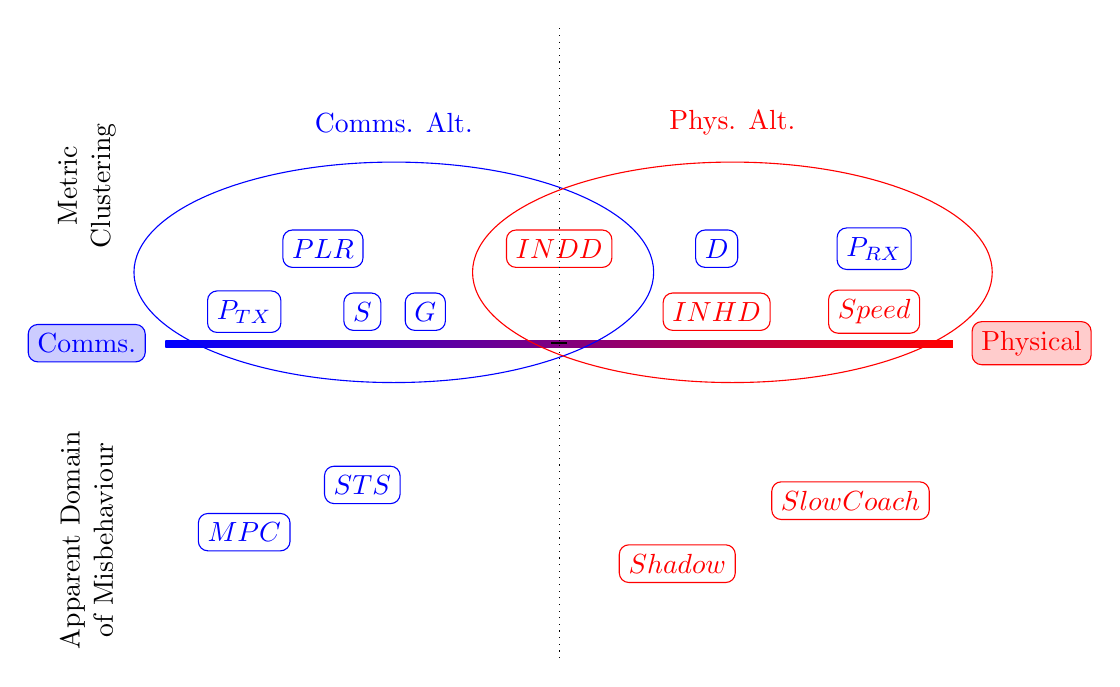
\begin{tikzpicture}[-latex,
    comms/.style={text=blue, draw=blue, rounded corners=.8ex},
    phys/.style={text=red, draw=red, rounded corners=.8ex}]
    % Start off with the line
    %\draw [<-|][comms, draw=blue, very thick] (0,1) -- (5,1); 
    %\draw [|->][phys, draw=red, very thick] (5,1) -- (10,1); 
    \path[left color=blue,right color=red]
    (0,0.95) rectangle +(10,2.5pt);

    % Baseline labels
    \node[comms, fill=blue, fill opacity=0.2, text opacity=1] at (-1,1) {Comms.};
    \node[phys, fill=red, fill opacity=0.2, text opacity=1] at (11,1) {Physical};

    % Metric Labels
    \node[comms] at (7,2.2) {$D$};
    \node[comms] at (9,2.2) {$P_{RX}$};
    \node[comms] at (1,1.4) {$P_{TX}$};
    \node[comms] at (2.5,1.4) {$S$};
    \node[comms] at (3.3,1.4) {$G$};
    \node[comms] at (2,2.2) {$PLR$};
    \node[phys] at (5,2.2) {$INDD$};
    \node[phys] at (7,1.4) {$INHD$};
    \node[phys] at (9,1.4) {$Speed$};

    \node[rotate=90, align=center] at (-1, 3) {Metric\\Clustering};
    \node[rotate=90, align=center] at (-1, -1.5) {Apparent Domain\\of Misbehaviour};
    \node[comms] at (1,-1.4) {$MPC$};
    \node[comms] at (2.5,-0.8) {$STS$};
    \node[phys] at (6.5,-1.8) {$Shadow$};
    \node[phys] at (8.7,-1) {$SlowCoach$};

    % Draw approx subsets
    \draw[comms] (2.9,1.9) ellipse (3.3 and 1.4);
    \draw[phys] (7.2,1.9) ellipse (3.3 and 1.4);

    \node[text=red] at (7.2,3.8) {Phys. Alt.};
    \node[text=blue] at (2.9,3.8) {Comms. Alt.};

    % Misc
    \draw[-|][dotted] (5,5) -- (5,1);
    \draw[-|][dotted] (5,-3) -- (5,1);


  \end{tikzpicture}
  \caption{Assumptions made about the relevant domains of impact / detectability of misbehaviours, and domain relevance of metrics, may not be optimal}
  \label{fig:alternate_domain_diag}
\end{figure}

\section{Optimal Metric Subset Analysis}
\todo{ADD: Subset Analysis}


\section{Conclusion}
In this chapter we demonstrate that in harsh environments, multi-domain trust assessment can perform better on average than single-domain counterparts, both in terms of robustness and sensitivity, but also covering a wider region of the potential behaviour space, 

The extension of the methodologies of multi-vector trust into the marine space are already demonstrated, however including information from physical observations of actors in a network enables the detection and identification of a much wider range of behaviours.
We also demonstrate a method for assessing trust metrics in harsh environments in terms of their relative significance, and a method for establishing classification signatures for misbehaviours.

It is to be noted that this presented method is significantly more computationally intensive than the relatively simple Hermes / OTMF algorithms communications only algorithms, and is exponential in complexity as metrics and/or domains are added. The repeated metric re-weighting required for real time behaviour detection is therefore an area that requires optimization. More work needs to be done to characterise how worthwhile this approach is compared to a separate synthesis approach where by MTFM-style trust is generated and assessed on a per-domain basis and subsequently fuzed.

For greater fidelity and more optimal results, a wider range of weights can be used in the initial regression step; however this is computationally expensive given that weighting is applied to each perspective (i.e.\ observer/target node pair) for each trust assessment time step, presenting 15 perspectives at each time interval in the 6 node case.

Every effort has been made to avoid over-training the dataset, using cross validating sampling for regression and "best weight" generation, however more meta-analysis is required to further demonstrate the functionality of this process.



%%%%%%%%%%%%%%%%%%%%%%%%%%%%%%%%%%%%%%%%%%%%%%%%%%%%%%%%%%%%%%%%%%%%%%%%%%%%%%%
 % Comparative Analysis of Multi-Comain Trust Assessment in Collaborative Module Networks

% !TeX spellcheck = en_GB
\def\ChapterTitle{Conclusions \& Future Work}

	\chapter{\ChapterTitle}
	\label{ch:conclusion}
	\lhead{Chapter \thechapter. \emph{\ChapterTitle}} % Write in your own chapter title to set the page header

\section{Conclusions}

The use of \gls{manet} architectures in the \gls{uan} space requires a fundamental reassessment of the security and reliability mechanisms and performance of such networks in the challenging underwater environment.
The strengths of \gls{manet} architectures inherently produce decentralised, self-organised, collaborative networks that strive towards efficiency and performance where all network members perform fairly.
However, with the increasing introduction of autonomy into the general \gls{manet} space, this assessment of ``fairness'' is simultaneously an assessment of the capability of the network, and of the ``trustworthiness'' of the autonomous nodes within it.

The original \gls{manet} architecture was designed with no in-built defence or security capabilities, and as such, threat mitigation mechanisms been superimposed over time to protect against fundamental vulnerabilities in the architecture due to assumptions of fairness, the use of open, wireless links with ``fuzzy'' operational boundaries, highly mobile nodes inducing dynamic topologies, and constrained power/computation/locomotion/communications resources.
These mechanisms vary, from evidence based cryptographic security such as centralised trusted third parties, a-priori shared secrets or one-time-pads, to fully decentralised \gls{pki} systems.
However, these classical security measures require significant investments in memory and computational power; communications channel occupancy; and inherently rely on relatively short delays between links and from end-to-end points in the network.

In the terrestrial realm, the increasing computing power of devices such as mobile phones has enabled the creation of pervasive, end to end security. 
However, as discussed in \autoref{ch:maritime_background}, these assumptions of channel availability and low-latency do not hold in the underwater acoustic space, which is massively variable in channel capacity and delay-response.
As such, regardless of on-board computing power, alternative, decentralised methods for ensuring the integrity of the network and its operations is essential for expanding the applications of \gls{manet} architectures in this space. 

These applications vary from defensive patrolling, \gls{asw} and \gls{mcm}, to pervasive environmental monitoring, and in almost all cases, current military and commercial implementations benefit from leveraging individual node autonomy in a distributed architecture to bring down development and operating costs, increase system efficiency, and fundamentally, save humans time and in extreme cases, lives. 

Trust is one alternative approach evidence based security to maintaining network integrity in the face of selfish, malicious or faulty misbehaviours in \glspl{manet}, and this approach has been well explored in the terrestrial realm.
In \autoref{ch:trust_background}, the fundamental concept of Trust was explored, and a range of psychological, phenomenological, and technical approaches to Trust assessment and collaborative Trust were investigated.
While this included excursions into the concepts of Design Trust (\autoref{sec:trust_perspectives}) and the impacts of human factors on the expected performance of trusting systems (\autoref{apx:human_factors}), this discussion was directed towards the application of Trust to autonomous \gls{manet}, as well as currently developed methods for establishing and maintaining trust in \glspl{manet} such as the Hermes and \gls{otmf} single-metric assessment frameworks (\autoref{sec:single_trust}), and \gls{mtfm}, which broke new ground in Trust establishment by looking at many available communications related metrics as an ensemble(\autoref{sec:multimetrictrust}), and applies Grey Relational Grading and whitenization (\autoref{apx:grey}) to take assessments across the communications domain and across the network topology to assess the trustworthiness of nodes within a \gls{manet} in a distributed fashion without requiring environmental or application specific ``training''.

In general, Trust is ``the level of confidence one agent has in another to perform a given action on request or in a certain context'' (\autoref{sec:trust_manets}), and has previously been exclusively concerned with the communications operations of networks, generally relying on measures of packet routing success to infer expectations of future packet delivery probabilities, improving route generation and mitigating threats from selfish or malicious interference (\autoref{sec:manet_vuln}).
However, the \gls{uan} application area and its challenging operation and communications constraints puts unique challenges on previous assumptions about the operation of abstract trust frameworks in \glspl{manet}, and as such required reassessment.

Further, the \gls{uan} application area also highlights more general challenges to Trust in autonomous \gls{manet}; with the imposition of a highly constrained communications channel, it is difficult to maintain sufficient information about the operation of nodes in the network with high enough regularity to reliably disseminate that information across the network.
Also, the high constrained physical dynamics and resource intensive communications and locomotion in \gls{uan} \glspl{manet} greatly expands the potential threat surface, particularly for \gls{dos}-style resource manipulation attacks; when locomotion is energetically expensive, if a node can selfishly get a ``free ride'' by minimising its mobility rather than fairly distributing effort across the network, operational mission times and overall efficiency can be impaired. 

As such there is an open opportunity to explore the application of Trust methodologies to the physical domain instead of and as well as the communications domain, making such a \glspl{tmf} able to identify a much greater range of potential misbehaviours and maintain both integrity and efficiency.


\section{Contributions and Findings}

Within this context, \autoref{ch:comms_trust} initially explores the scaling differences in node distance and communications rates using a simulated agent based environmental and communications model, identifying network saturation rates using a range of mobility, scaling, and offered loads, maximising network performance in terms of a throughput-delay product.
Existing \glspl{tmf} methods are applied to this established range, demonstrating that these (Hermes, \gls{otmf} and \gls{mtfm}) existing frameworks are not directly suitable to the sparse, noisy, and dynamic underwater environment.
While there is little that can be done to augment Hermes and \gls{otmf} in this environment, the weighted-metric nature of \gls{mtfm} allows the metric space to be explored for ``better'' weighting vectors to detect and identify misbehaviours that are hidden in the unweighted assessment.

Having established the operation of Trust in the marine \gls{manet} environment, \autoref{ch:physical_trust} demonstrates through statistical measures of node distribution and velocities, that malicious and faulty misbehaviours can be both detected and identified to a high selectivity using a simple tree-based classifier, using a collaborative Port Protection scenario as a targeted waypoint mobility baseline.

In \autoref{ch:multi_domain}, the combination of these domains is assessed.
The relative significance of metrics in the specific identification of a given behaviour is performed through a full-sight random forest regression by comparing a significant number of simulated mission runs.
These significances, while simply a statistical measure of the importance of a given metric in discriminating between two behaviour (i.e. a fair behaviour and the misbehaviour) provide actionable information to generate a weighted metric sequence targeting that behaviour.
The identification and classification methodologies from both \autoref{ch:comms_trust} and \autoref{ch:physical_trust} are combined to generate a classifier with very beneficial performance.


\section{Future Work}
One of the fundamental difficulties in establishing trust in sparse, noisy networks is that it takes a significant amount of time to accumulate enough observational metric data to for actionable opinions.
This problem is exacerbated by the asynchronous nature of those metrics; this is evident in the multi-domain discussion between communications and physical metrics where overheard location updates for a given node my arrive out-of-sync from other useful information about that particular relationship, but is also the case in the pure communications domain.

If these metrics are not synchronised, for instance if they are interrupt driven such as communications-based observations, generating more abstract measurements requires inherent assumptions about ``how to accumulate the data while you wait''. 
For instance, \autoref{ch:comms_trust} and \cite{Bolster2015} demonstrated a periodic trust assessment framework for autonomous marine environments, in such an environment, to establish useful, generalised, data, it was necessary to wait for a relatively long time to accumulate enough data to make assessments.
However, this leads to data being left in-buffer for a time before being used to make decisions, and by the time the data was collated and processed, it could be wildly different from the reality. 
Further, while some periods could be extremely sparse or even empty, others could be extremely busy with many records having to be averaged down to provide a 'single period' response. 
One solution to this would be to move from a stepping-window of trust observations as used in this work to a continuous trust log, updated on packet reception rather than waiting regular periods for packets to be analysed.
Therefore, the implementation of a suitable grey sequence buffer version of the framework would be beneficial.

Such a sequence buffer framework would involve a tracking predictor that would provide best-guess estimates of an interpolated value for a metric between value updates, and a back-propagation algorithm to retroactively update historical assessments of that metrics so as to better inform any abstracted trust value predictor.

Additionally, future work could investigate the improvement of weight-based detection algorithms, the stability of \gls{gra} under multi-node collusion, the development of real-time outlier detection on physical platforms.

From \autoref{ch:physical_trust}, it is recognised that the geometric abstractions used to assess the validity of ``physical trust assessment'' are application-agnostic (assuming collaborative mobility) and the applicability of this assessment and detection method to other areas such as \gls{auv} operations or Autonomous Vehicle Networks, potentially forming a mode of ``body language'' verification for autonomous systems. 
Equally, the selected metrics are by no means exhaustive, and other application / mobility specific metrics, such as deviation from a planned path rather than deviation from a current-node-centre, would benefit the field.

A similarly enticing area of research is the impact of variable misbehaviour will have on such multi-domain approaches; taking the \gls{mpc} behaviour as an example, a time-variant power emphasis could evade windowed trust assessment.

With respect to the operational performance impacts of physical misbehaviour, this is a very unexplored space and it's possible that the selected misbehaviours were too unambitious; future work will have to investigate the impact of ``heavy-handed'' or destructive behaviours on the operational efficiency of autonomous networks.

One disappointing issue with these results presented in \autoref{ch:multi_domain} is that the \gls{sts} behaviour has been stubbornly avoiding identification in the ``live'' multi-domain space while presenting ostensibly discernible metric significances in the comparison space. 
However the performance of the remaining targeted synthetic domains indicates that this is a valid result and that the methodology is sound, if in need of some refinement and corroboration.
It is possible that the outlying results used in the initial training set are simply too noisy to accurately optimise towards \gls{sts} directly and this analysis is victim of over-fitting. 
On the other hand, the fact that it is the only misbehaviour that is purely application-level indicates that there is potential to further expand this methodology to include some traffic inspection and logical link tracking as an additional ``routing'' level domain to explore irregularities in traffic patters in addition to the largely physical-communication-domain metrics currently used.

As with any trust framework, the effects of different contexts, misbehaviours, and environments are an interesting area.
In this case, where we are primarily concerned with the interplay and usefulness of trust between domains, the generation of new/other misbehaviours (particularly attacks on the physical domain or cross-domain attacks) would provide insights and either validation or invalidation to the presented optimisation methodology when applied to ``Blind'' behaviours, or applying the final ``Mean'' synthetic to a range of totally untrained behaviours.

\section{Summary}

In this thesis, the operation of trust in the challenging \gls{uan} environment was explored, demonstrating that without augmentation, current \gls{tmf} approaches do not perform well.
A novel approach to Trust was demonstrated, using physical metrics as a raw trust assessment metric source.
Finally, a metric weight optimisation methodology was demonstrated to automatically develop trust weightings that highlight a given misbehaviour, driving its targeted trust low so as to enable detection by even simple classifiers.

Overall, the approaches taken throughout this thesis are largely application agnostic and are indeed domain-agnostic; it has been demonstrated that the use of trust assessment across communications and physical domains yields beneficial results, but the same approach could be applied to non-physical autonomous agents such as high-frequency trading initiatives, forensic accounting/auditing,  cheat-detection in online gaming, lane-assistance in self-driving cars, and possibly most interesting, having the autonomous agents assess how trust-worthy we are across domains such as vocal tonality, facial expressions, ``body language'', and other biometric factors in addition to just the words or commands we use.
So, should they trust us? % Conclusion

%% ----------------------------------------------------------------
% Now begin the Appendices, including them as separate files

\addtocontents{toc}{\vspace{2em}} % Add a gap in the Contents, for aesthetics

\appendix % Cue to tell LaTeX that the following 'chapters' are Appendices

% Appendix B - Human Factors

\chapter{Human Factors related to Trusted Operation of Autonomous Systems}
\label{apx:human_factors}
\lhead{Appendix \thechapter. \emph{Human Factors related to Operational Trust}}

This work has largely considered autonomous systems as entities of wider systems, implicitly involving human operators/agents in some part of the desired operation.
We refer to these systems as \gls{acs}.
As described in~\autoref{Chapter3}, Operational Trust has two main aspects, trust in the system to behave as expected and trust in the interfaces between systems (human/machine and machine/machine).
Of all of the interfaces in an Autonomous Collaborative System, the most problematic is that arguably that between the \gls{acs} and the human operator / team of operators.
Cummings identified the main challenges to \gls{hsc}, summarised below:\cite{Cummings2010}

\section{Information Overload}
Operator efficiency exhibits an optimum at moderate levels of cognitive engagement, above which cognitive ability is overloaded and performance drops (Otherwise known as the Yerkes-Dodson Law).
Additionally, in the case of under-engagement, operators can fall foul of boredom, and become desensitised to changing factors.
\textit{However, predicting this point of over-saturation is an open psychophysiological research problem.}

\section{Adaptive Automation}
Automation is well tailored to consistent levels of activity.
This is quite simply not the case many domains.
Particularly in defence and military applications, activity is characterised by long periods of ``routine'' punctuated by high intensity, usually unpredictable, activity.
At those interfaces between ``calm'' and ``storm'', where real time situational awareness is imperative, temporary Information Overload is highly probable.
Adaptive Automation enables autonomous systems to increase their \gls{loa} based on specific events in the task environment, changes in operator performance or task loading, or physiological methods.
It is taken as given that for routine operations, and increased \gls{loa} reduces operator workload, and vice versa.
However, this relationship is highly task dependent and can create severe problems in cases of \gls{loa} being greater, or indeed lesser, than is required.
In the cases of overly-high \gls{loa}, operator skill is degraded, situational awareness is reduced as the operator is not as engaged, and the automated system may not be able to handle unexpected events, requiring the operator to take over, which, given the previous points, is a difficult prospect.
Alternatively, in sub-optimal \gls{loa}, Information Overload can result in the case of high intensity situations, but also the system can fall foul of overly-sensitive human cognitive biases, false positive pattern detection, boredom, and complacency in the case where less is going on.
Therefore, as a corollary to Information Overload challenges, there is a need to define the interrelationship between levels of situational activity (or risk) and appropriate levels of automation.
\textit{Under what circumstances can AA be used to change the \gls{loa} of a system?
Does the autonomous system or the human decide to change \gls{loa}\@? 
What \gls{loa}s are appropriate for what circumstances?}

\section{Distributed Decision Making}
In a modern, non-hierarchical, often distributed or cellular military management system (Network Centric Warfare doctrine for example), tools are increasingly being used to mitigate information asymmetry within command and control.
A simple example of this is shared watch-logs in Naval operations, providing temporal collaboration between watch-teams separated in time.
The DoD Global Information Grid is another example of a spatial collaborative framework.
Recent work has demonstrated the power of collaborative analysis and human-machine shared sensing technologies even with low levels of training on the part of the operators providing superior results and resource efficiencies than either humans or machines alone in survey and search-and-rescue scenarios (Ahmed et al.2014)\todo{Check Security}.
As these temporal and spatial collaboration tools increase in complexity and ability, decisions that previously required SA that was only available at higher echelons within the standard hierarchy are available to commanders on the ground, or even to individual team members, enabling the potential for informed decisions to be taken faster and more effectively, enabled by automated strategies to present relevant information to teams based on the operational context.
However there are a range of operational, legal, psychological and technical challenges that need to be addressed before confidence in these distributed management structures can be established.
Studies into situational awareness sharing techniques (telepresent table-top environments, video conferencing, and interactive whiteboards) have generally yielded positive results, however investigations into interruptive-communications (such as instant messaging chat) have demonstrated a negative impact on operational efficiency.
In short, the biggest problem with distributed decision making in the context of supervisory systems is that \textit{there is no consensus on whether it is advantageous or not, and what magnitude of operational delta is introduced, if any.}

\section{Complexity}
Beyond simple Information Overload, increasing complexity of information presented to operators is having a negative effect on operational efficiency.
In HSC, displays are designed to reduce complexity, introducing abstractions with an aim to presenting the minimum amount of information to the operator required to maintain an accurate and up-to-date mental model of the environmental and operational state.
This has led to the development of many domain specific decision support interfaces, however, in academic research, there has been nothing but ‘mixed results’.
One commonly raised negative is the general bias on the ‘cool factor’ of interfaces.
Immersive 3D visual, aural, or haptic interfaces that at first appraisal seem to provide more approachable information to the operator, and are indeed tacitly preferred by operators in use.
However, there has not been any evidence to demonstrate performance improvement when using these tools, and in-fact, \textit{improving the ``fidelity'' of the interfaces has led to operators’ overly-relying on these representations of the environment rather than remaining engaged in the environment.}

\section{Cognitive Biases and Failing Heuristics}
In many areas, operators and commanders are required to make rapid decisions with imperfect information, driven by massively increased information availability and rates of change in areas such as battlefield tactics and global finance markets.
However, Human decision making isn’t always rational (especially under pressure), and operators use personally derived heuristics to make ``rational shortcuts''.
This is a double edged sword, where these heuristics can be employed to greatly reduce the normative cognitive load in a stressful situation, but also introduce destructive biases, where these shortcuts make assumptions that don’t bear out in reality.

For example, in the context of decision support systems, ``Autonomy Bias'' has been observed as a complement to the already well known ``Confirmation Bias''\footnote{Confirmation Bias is the tendency for people to preferentially select from available information that information that supports pre-existing beliefs or hypotheses.}  and ``Assimilation Bias''\footnote{Assimilation Bias is often thought of as a subset of Confirmation Bias, whereby it specifies that instead of seeking out information supporting of current views, any incoming data is interpreted as being supportive of a particular view without questioning that view, even if it appears contradictory.}, where operators that have been provided with a ``correct'' answer by a decision support system do not look (or see, depending on perspective) for any contradictory information, and will unquestionably follow, increasing error rates significantly.

This behaviour isn't only the reserve of decision support systems, but also in the generic allocation of operator attention; scheduling heuristics are used to decide how much time tasks should be worked on, and time and again, humans are found to be far from optimal in this regard, especially in time-pressured scenarios where these heuristics are in even more demand.
Even when operators are given optimal scheduling rules, these quickly fall apart, often due to primary task efficiency degradation after interruption.
This highlights a critical interface in the adoption of complex autonomous systems that still demand ‘Man in the loop’ functionality; if a system is required to have full-time concentrated supervision (e.g.\ flying a UCAV), but also event-based reactive decision making (e.g.\ alerts from non-critical subsystems), both tasks are negatively impacted.
In an assessment of factors influencing trust in autonomous vehicles and medical diagnosis support systems, Carlson et al also identified that a major factor in an operator or users’ trust in a system was not only dependant on past performance and current accuracy but also on ``soft factors'' such as the branding and reputation of the manufacture / designer. (Carlson et al. 2014)\todo{Check Security}
Further, autonomous decision support / detection / classification systems have an ``uncanny valley'' to overcome in terms of accuracy, in that there is a dangerous period when such systems are used but not perfect, but operators become complacent, causing an increased error rate, until such a time that those autonomous systems can match or exceed the detection rates of their human counterparts.
 % Appendix Title

% Appendix C - Grey Theory

\chapter{Grey System Theory and Grey Trust Assessment}
\label{apx:grey}
\lhead{Appendix \thechapter. \emph{Grey System Theory and Grey Trust Assessment}}

\section{Grey numbers, operators and terminology}
Grey numbers are used to represent values where their discrete value is unknown, where that number may take its possible value within an interval of potential values, generally written using the symbol $\oplus$.
Taking $a$ and $b$ as the lower and upper bounds of the grey interval respectively, such that $\oplus \in [a,b] | a < b$ 
The ``field'' of $\oplus$ is the value space $[a,b]$.
There are several classes of grey numbers based on the relationships between these bounds.
Black and White numbers are the extremes of this classification; such that $\dot\oplus \in [-\infty, +\infty]$ and $\mathring\oplus \in [x, x] | x \in \mathbb{R}$ or $\oplus(x)$
It is clear that white numbers such as $\mathring\oplus$ have a field of zero while black numbers have an infinite field.

Grey numbers can also represent partial knowledge about a system or metric, and as such can represent half-open concepts, by only defining a single bound; for example $\underline\oplus = \oplus(\underline x ) \in [x, +\infty]$ and $\overline\oplus = \oplus(\overline x) \in [-\infty, x]$.

Primary operations within this number system are as follows;
\begin{subequations}
  \begin{align}
    \oplus_1 + \oplus_2      &\in [a_1+a_2,b_1+b_2] \label{eq:grey_add}\\
    -\oplus         &\in [-b,-a] \label{eq:grey_neg} \\
    \oplus_1 - \oplus_2      &= \oplus_1+(-\oplus) \label{eq:grey_sub}\\
    \oplus_1 \times \oplus_2 &\in \begin{aligned}[t]
      &[\min(a_1 a_2, a_1 b_2, b_1 a_2, b_2 a_2), \\
      & \max(a_1 a_2, a_1 b_2, b_1 a_2, b_2 a_2)]
    \end{aligned} \label{eq:grey_mult}\\
    \oplus^{-1} &\in [b^{-1}, a^{-1}] \label{eq:grey_inv}\\
    \oplus_1 / \oplus_2 & = \oplus_1 \times \oplus_2^{-1} \label{eq:grey_div} \\
    \oplus \times k &\in [ka,kb] \label{eq:grey_times_scalar}\\
    \oplus^k &\in [a^k, b^k] \label{eq:grey_exp}
  \end{align}
\end{subequations}
where $k$ is a scalar quantity.

\section{Whitenisation and the Grey Core}
The characterisation of grey numbers is based on the encapsulation of information in a grey system in terms of the grey numbers core ($\hat\oplus$) and it's degree of greyness ($g^\circ$).
If the distribution of a grey number field is unknown and continuous, $\hat\oplus = \frac{a + b}{2}$.

Non-essential grey numbers are those that can be represented by a white number obtained either through experience or particular method~\cite{Liu2011}.
This white value is represented by $\tilde\oplus$ or $\oplus(x)$ to represent grey numbers with $x$ as their whitenization.
In some cases depending on the context of application, particular grey numbers may temporarily have no reasonable whitenisation value (for instance, a black number).
Such numbers are said to be Essential grey numbers.
\begin{comment}
\section{Grey Sequence Buffers and Generators}
\todo{eqs of sequence buffers and partial derivs}
Given a fully populated value space, sequence buffer operations are used to provide abstractions over the dataspace.
These abstractions can be \emph{weakening} or \emph{strengthening}.
In the weakening case, these operations perform a level of smoothing on the volatility of a given input space, and strengthening buffers serve to highlight and 
A powerful tool in grey system theory is the use of grey incidence factors, comparing the ``likeness'' of one value against a cohort of values.
This usefulness applies particularly well in the case of multi-agent trust networks, where the aim is to detect and identify malicious or maladaptive behaviour, rather than an absolute assessment of ``trustworthiness''.
\end{comment}

\section{Application of Grey Relational Grading to Trust}
Grey Relational Grading performs cohort based normalization of metrics at runtime.
This creates a more stable contextual assessment, providing a ``grade'' of trust compared to other observed entities in that interval, while maintaining the ability to reduce values to a stable assessment range for decision support without requiring every environment entered into to be characterised.
Grey assessments are relative in both fairly and unfairly operating cohorts.
Entities will receive mid-range trust assessments if there are no malicious actors as there is no-one else ``bad'' to compare against.

\citet{Guo11} demonstrated the ability of Grey Relational Analysis (GRA)\cite{Zuo1995} to normalise and combine disparate traits of a communications link such as instantaneous throughput, received signal strength, etc.\ into a Grey Relational Coefficient, or a ``trust vector''.
In \cite{Guo11}, the observed metric set $X = {x_1,\dots,x_M}$ representing the measurements taken by each node of its neighbours at least interval, is defined as $X=[$packet loss rate, signal strength, data rate, delay, throughput$]$.
The Grey Relational Grade is given as
%
\begin{align}
  %\label{eq:grc}
  \theta_{k,j}^t = \frac{\min_k|a_{k,j}^t - g_j^t| + \rho \max_k|a_{k,j}^t-g_j^t|}{|a_{k,j}^t-g_j^t| + \rho \max_k|a_{k,j}^t-g_j^t|} \\
  \phi_{k,j}^t = \frac{\min_k|a_{k,j}^t - b_j^t| + \rho \max_k|a_{k,j}^t-b_j^t|}{|a_{k,j}^t-b_j^t| + \rho \max_k|a_{k,j}^t-b_j^t|} \notag 
\end{align}
%
where $a_{k,j}^t$ is the value of a observed metric $x_j$ for a given node $k$ at time $t$, $\rho$ is a distinguishing coefficient, usually set to $0.5$, $g$ and $b$ are respectively the '``good'' and ``bad'' reference metric sequences from $\{a_{k,j}^t k=1,2\dots K\}$, e.g.\ $g_j=\max_k({a_{k,j}^t})$,  $b_j=\min_k({a_{k,j}^t})$ (where each metric is selected to be monotonically positive for trust assessment, e.g.\ higher throughput is always better).

Weighting can be applied before generating a scalar value which allows the identification and classification of untrustworthy behaviours.

%
\begin{equation}
  %\label{eq:metric_weighting}
  [\theta_k^t, \phi_k^t] = \left[\sum_{j=0}^M h_j \theta_{k,j}^t,\sum_{j=0}^M h_j \phi_{k,j}^t \right]
\end{equation}
Where $H=[h_0\dots h_M]$ is a metric weighting vector such that $\sum h_j = 1$, and in the basic case, $H=[\frac{1}{M},\frac{1}{M}\dots\frac{1}{M}]$ to treat all metrics evenly.
$\theta$ and $\phi$ are then scaled to $[0,1]$ using the mapping $y = 1.5 x - 0.5$.
The $[\theta,\phi]$ values are reduced into a scalar trust value by $T_k^t = ({1+{(\phi_k^t)^2}/{(\theta_k^t)^2}})^{-1}$.
This trust value minimises the uncertainties of belonging to either best ($g$) or worst ($b$) sequences in \eqref{eq:grc}.

\acrshort{mtfm} combines this \gls{gra} with a topology-aware weighting scheme\eqref{eq:networkeffects} and a fuzzy whitenization model\eqref{eq:whitenization}.
There are three classes of topological trust relationship used; Direct, Recommendation, and Indirect.
Where an observing node, $n_i$, assesses the trust of another, target, node, $n_j$; the Direct relationship is $n_i$'s own observations $n_j$'s behaviour.
In the Recommendation case, a node $n_k$, which shares Direct relationships with both $n_i$ and $n_j$, gives its assessment of $n_j$ to $n_i$.
The Indirect case, similar to the Recommendation case, the recommender $n_k$, does not have a direct link with the observer $n_i$ but $n_k$ has a Direct link with the target node, $n_j$.
These relationships give us node sets, $N_R$ and $N_I$ containing the nodes that have recommendation or indirect, relationships to the observing node respectively.
%
\begin{align}
  %\label{eq:networkeffects}
  T_{i,j}^{\acrshort{mtfm}}=\frac{1}{2} \cdot \max_s\{f_s(T_{i,j})\} T_{i,j}+&\frac{1}{2} \frac{2|N_R| }{2|N_R| + |N_I|}\sum_{n \in N_R} \max_s\{f_s(T_{i,n})\} T_{i,n}\\ \notag
  +&\frac{1}{2} \frac{|N_I| }{2|N_R| + |N_I|}\sum_{n \in N_I} \max_s\{f_s(T_{i,n})\} T_{i,n} 
\end{align}
Where $T_{i,n}$ is the subjective trust assessment of $n_i$ by $n_n$, and $f_s = [ f_1,f_2, f_3]$ given as:
\begin{align}
  %\label{eq:whitenization}
  f_1(x)&= -x+1\notag\\
  f_2(x)&= 
  \begin{cases}
    2x & \text{if }x\leq 0.5\\
    -2x+2 & \text{if }x>0.5
  \end{cases}\\
  f_3(x)&= x\notag
\end{align}

Grey System Theory, by it's own authors admission, hasn't taken root in it's originally intended area of system modelling \cite{Liu2011}.
However, given it's tentative application to \gls{manet} trust, taking a Grey approach on a per metric benefit has qualitative benefits that require investigation; the algebraic approach to uncertainty and the application of ``essential and non essential greyness'', whiteisation, and particularly grey buffer sequencing allow for the opportunity to generate continuous trust assessments from multiple domains asynchronously.

\todo{NORELEASE: Wrap up the grey discussion}

\section{UNEDITED PROSE: Real Time Grey Systems}
\emph{Incoming Train of Consciousness}


For a given metric set $X$ such that $X = {x_1,\dots,x_M}$ representing the $M$ different types of measurement generated by an observer. If these metrics are not synchronised, for instance if they are interrupt driven such as communications-based observations, generating more abstract measurements requires inherent assumptions about ``how to accumulate the data while you wait''. For instance, in \cite{Bolster2015}, we demonstrated a periodic trust assessment framework for autonomous marine environments, in such an environment, to establish useful, generalised, data, it was necessary to wait for a relatively long time to accumulate enough data to make assessments.
However, this left many 'smells'; data was being left in-buffer for a long time before being used to make decisions, and by the time the data was collated and processed, it could be wildly different from the reality. Further, while some periods could be extremely sparse or even empty, others could be extremely busy with many records having to be averaged down to provide a 'single period' response. 
Therefore, the implementation of a suitable sequence buffer version of the framework would be beneficial.

Such a sequence buffer framework would involve a tracking predictor that would provide best-guess estimates of an interpolated value for a metric between value updates, and a back-propagation algorithm to retroactively update historical assessments of that metrics so as to better inform any abstracted trust value predictor.

I had initially thought that such a back-propagator would be a total mess as I'd imagined that significant-model-breaking would potentially indicate untrustworthy behaviour, but this is stupid since the per-metric-model has the least information of anyone and is simply there to provide better intermediate values and has no / limited direct impact on the overall trust behaviour. 

This back propagation will probably be a pain to implement as it'd require a retroactive reassessment of trust and could get really messy if it was interrupt driven, but it's better not to prematurely optimise.


 % Appendix Title

% Ophaned Sections

\chapter{Orphan Sections}
\label{apx:orphans}
\lhead{Appendix \thechapter. \emph{Orphan Sections}}	% Appendix Title

% vim:ft=tex:
%
% Appendix D

\chapter{Additional Graphs}
\label{apx:graph_overflow}
\lhead{Appendix \thechapter. \emph{Additional Graphs}}

\section{From \autoref{sec:weight_assessment}: Mean-Weighted Multi-Domain Trust Results}\label{sec:apx_mean_targeting_malicious}


These graphs show the trust variability of an individiual against a mean-averaged trust response of the remaining cohort of nodes.


%%%%%%%%%%%%%%%%%%%%%%%%%%%%%%%%%%%%%%%%%%%%%%%%%%%%%%%%%%%%%%%%%%%%%%%%%%%%% MEAN PLOTS BELOW

\begin{figure}[h]
  \centering
  \includegraphics[width=\linewidth]{best_comms_run_instantaneous_MPC}
  \caption{\gls{mpc} Comms Metric Trust (showing mean of non-misbehaving nodes)}
  \label{fig:comms_instantaneous_mpc}
\end{figure}

\begin{figure}[h]
  \centering
  \includegraphics[width=\linewidth]{best_phys_run_instantaneous_MPC}
  \caption{\gls{mpc} Physical Metric Trust (showing mean of non-misbehaving nodes)}
  \label{fig:phys_instantaneous_mpc}
\end{figure}

\begin{figure}[h]
  \centering
  \includegraphics[width=\linewidth]{best_full_run_instantaneous_MPC}
  \caption{\gls{mpc} Full Metric Trust (showing mean of non-misbehaving nodes)}
  \label{fig:full_instantaneous_mpc}
\end{figure}


\begin{figure}[h]
  \centering
  \includegraphics[width=\linewidth]{best_comms_run_instantaneous_STS}
  \caption{\gls{sts} Comms Metric Trust (showing mean of non-misbehaving nodes)}
  \label{fig:comms_instantaneous_sts}
\end{figure}

\begin{figure}[h]
  \centering
  \includegraphics[width=\linewidth]{best_phys_run_instantaneous_STS}
  \caption{\gls{sts} Physical Metric Trust (showing mean of non-misbehaving nodes)}
  \label{fig:phys_instantaneous_sts}
\end{figure}

\begin{figure}[h]
  \centering
  \includegraphics[width=\linewidth]{best_full_run_instantaneous_STS}
  \caption{\gls{sts} Full Metric Trust (showing mean of non-misbehaving nodes)}
  \label{fig:full_instantaneous_sts}
\end{figure}



\begin{figure}[h]
  \centering
  \includegraphics[width=\linewidth]{best_comms_run_instantaneous_Shadow}
  \caption{Shadow Comms Metric Trust (showing mean of non-misbehaving nodes)}
  \label{fig:comms_instantaneous_shadow}
\end{figure}

\begin{figure}[h]
  \centering
  \includegraphics[width=\linewidth]{best_phys_run_instantaneous_Shadow}
  \caption{Shadow Physical Metric Trust (showing mean of non-misbehaving nodes)}
  \label{fig:phys_instantaneous_shadow}
\end{figure}

\begin{figure}[h]
  \centering
  \includegraphics[width=\linewidth]{best_full_run_instantaneous_Shadow}
  \caption{Shadow Full Metric Trust (showing mean of non-misbehaving nodes)}
  \label{fig:full_instantaneous_shadow}
\end{figure}



\begin{figure}[h]
  \centering
  \includegraphics[width=\linewidth]{best_comms_run_instantaneous_SlowCoach}
  \caption{SlowCoach Comms Metric Trust (showing mean of non-misbehaving nodes)}
  \label{fig:comms_instantaneous_slowcoach}
\end{figure}

\begin{figure}[h]
  \centering
  \includegraphics[width=\linewidth]{best_phys_run_instantaneous_SlowCoach}
  \caption{SlowCoach Physical Metric Trust (showing mean of non-misbehaving nodes)}
  \label{fig:phys_instantaneous_slowcoach}
\end{figure}

\begin{figure}[h]
  \centering
  \includegraphics[width=\linewidth]{best_full_run_instantaneous_SlowCoach}
  \caption{SlowCoach Full Metric Trust (showing mean of non-misbehaving nodes)}
  \label{fig:full_instantaneous_slowcoach}
\end{figure}

\clearpage

\section{From \autoref{sec:weight_assessment}: Multi-Domain Trust Results Targeting Non-malicious nodes}

\subsection{Per Node Breakdowns}\label{sec:apx_targeting_non_malicious}
\begin{figure}[h]
  \centering
  \includegraphics[width=\linewidth]{best_comms_run_alt_time_MPC}
  \caption{\gls{mpc} Comms Metric Trust (targeting non-malicious node)}
  \label{fig:comms_alt_time_mpc}
\end{figure}

\begin{figure}[h]
  \centering
  \includegraphics[width=\linewidth]{best_phys_run_alt_time_MPC}
  \caption{\gls{mpc} Physical Metric Trust (targeting non-malicious node)}
  \label{fig:phys_alt_time_mpc}
\end{figure}

\begin{figure}[h]
  \centering
  \includegraphics[width=\linewidth]{best_full_run_alt_time_MPC}
  \caption{\gls{mpc} Full Metric Trust (targeting non-malicious node)}
  \label{fig:full_alt_time_mpc}
\end{figure}


\begin{figure}[h]
  \centering
  \includegraphics[width=\linewidth]{best_comms_run_alt_time_STS}
  \caption{\gls{sts} Comms Metric Trust (targeting non-malicious node)}
  \label{fig:comms_alt_time_sts}
\end{figure}

\begin{figure}[h]
  \centering
  \includegraphics[width=\linewidth]{best_phys_run_alt_time_STS}
  \caption{\gls{sts} Physical Metric Trust (targeting non-malicious node)}
  \label{fig:phys_alt_time_sts}
\end{figure}

\begin{figure}[h]
  \centering
  \includegraphics[width=\linewidth]{best_full_run_alt_time_STS}
  \caption{\gls{sts} Full Metric Trust (targeting non-malicious node)}
  \label{fig:full_alt_time_sts}
\end{figure}



\begin{figure}[h]
  \centering
  \includegraphics[width=\linewidth]{best_comms_run_alt_time_Shadow}
  \caption{Shadow Comms Metric Trust (targeting non-malicious node)}
  \label{fig:comms_alt_time_shadow}
\end{figure}

\begin{figure}[h]
  \centering
  \includegraphics[width=\linewidth]{best_phys_run_alt_time_Shadow}
  \caption{Shadow Physical Metric Trust (targeting non-malicious node)}
  \label{fig:phys_alt_time_shadow}
\end{figure}

\begin{figure}[h]
  \centering
  \includegraphics[width=\linewidth]{best_full_run_alt_time_Shadow}
  \caption{Shadow Full Metric Trust (targeting non-malicious node)}
  \label{fig:full_alt_time_shadow}
\end{figure}



\begin{figure}[h]
  \centering
  \includegraphics[width=\linewidth]{best_comms_run_alt_time_SlowCoach}
  \caption{SlowCoach Comms Metric Trust (targeting non-malicious node)}
  \label{fig:comms_alt_time_slowcoach}
\end{figure}

\begin{figure}[h]
  \centering
  \includegraphics[width=\linewidth]{best_phys_run_alt_time_SlowCoach}
  \caption{SlowCoach Physical Metric Trust (targeting non-malicious node)}
  \label{fig:phys_alt_time_slowcoach}
\end{figure}

\begin{figure}[h]
  \centering
  \includegraphics[width=\linewidth]{best_full_run_alt_time_SlowCoach}
  \caption{SlowCoach Full Metric Trust (targeting non-malicious node)}
  \label{fig:full_alt_time_slowcoach}
\end{figure}

\clearpage

\subsection{Averaged across remaining cohort}\label{sec:apx_mean_targeting_non_malicious}

\begin{figure}[h]
  \centering
  \includegraphics[width=\linewidth]{best_comms_run_alt_instantaneous_MPC}
  \caption{\gls{mpc} Comms Metric Trust (targeting non-malicious node, showing mean of remaining cohort including malicious node)}
  \label{fig:comms_alt_instantaneous_mpc}
\end{figure}

\begin{figure}[h]
  \centering
  \includegraphics[width=\linewidth]{best_phys_run_alt_instantaneous_MPC}
  \caption{\gls{mpc} Physical Metric Trust (targeting non-malicious node, showing mean of remaining cohort including malicious node)}
  \label{fig:phys_alt_instantaneous_mpc}
\end{figure}

\begin{figure}[h]
  \centering
  \includegraphics[width=\linewidth]{best_full_run_alt_instantaneous_MPC}
  \caption{\gls{mpc} Full Metric Trust (targeting non-malicious node, showing mean of remaining cohort including malicious node)}
  \label{fig:full_alt_instantaneous_mpc}
\end{figure}


\begin{figure}[h]
  \centering
  \includegraphics[width=\linewidth]{best_comms_run_alt_instantaneous_STS}
  \caption{\gls{sts} Comms Metric Trust (targeting non-malicious node, showing mean of remaining cohort including malicious node)}
  \label{fig:comms_alt_instantaneous_sts}
\end{figure}

\begin{figure}[h]
  \centering
  \includegraphics[width=\linewidth]{best_phys_run_alt_instantaneous_STS}
  \caption{\gls{sts} Physical Metric Trust (targeting non-malicious node, showing mean of remaining cohort including malicious node)}
  \label{fig:phys_alt_instantaneous_sts}
\end{figure}

\begin{figure}[h]
  \centering
  \includegraphics[width=\linewidth]{best_full_run_alt_instantaneous_STS}
  \caption{\gls{sts} Full Metric Trust (targeting non-malicious node, showing mean of remaining cohort including malicious node)}
  \label{fig:full_alt_instantaneous_sts}
\end{figure}



\begin{figure}[h]
  \centering
  \includegraphics[width=\linewidth]{best_comms_run_alt_instantaneous_Shadow}
  \caption{Shadow Comms Metric Trust (targeting non-malicious node, showing mean of remaining cohort including malicious node)}
  \label{fig:comms_alt_instantaneous_shadow}
\end{figure}

\begin{figure}[h]
  \centering
  \includegraphics[width=\linewidth]{best_phys_run_alt_instantaneous_Shadow}
  \caption{Shadow Physical Metric Trust (targeting non-malicious node, showing mean of remaining cohort including malicious node)}
  \label{fig:phys_alt_instantaneous_shadow}
\end{figure}

\begin{figure}[h]
  \centering
  \includegraphics[width=\linewidth]{best_full_run_alt_instantaneous_Shadow}
  \caption{Shadow Full Metric Trust (targeting non-malicious node, showing mean of remaining cohort including malicious node)}
  \label{fig:full_alt_instantaneous_shadow}
\end{figure}



\begin{figure}[h]
  \centering
  \includegraphics[width=\linewidth]{best_comms_run_alt_instantaneous_SlowCoach}
  \caption{SlowCoach Comms Metric Trust (targeting non-malicious node, showing mean of remaining cohort including malicious node)}
  \label{fig:comms_alt_instantaneous_slowcoach}
\end{figure}

\begin{figure}[h]
  \centering
  \includegraphics[width=\linewidth]{best_phys_run_alt_instantaneous_SlowCoach}
  \caption{SlowCoach Physical Metric Trust (targeting non-malicious node, showing mean of remaining cohort including malicious node)}
  \label{fig:phys_alt_instantaneous_slowcoach}
\end{figure}

\begin{figure}[h]
  \centering
  \includegraphics[width=\linewidth]{best_full_run_alt_instantaneous_SlowCoach}
  \caption{SlowCoach Full Metric Trust (targeting non-malicious node, showing mean of remaining cohort including malicious node)}
  \label{fig:full_alt_instantaneous_slowcoach}
\end{figure}


 % Appendix Title

\todototoc
\listoftodos

\addtocontents{toc}{\vspace{2em}}  % Add a gap in the Contents, for aesthetics
\backmatter

%% ----------------------------------------------------------------
\label{Bibliography}
\lhead{\emph{Bibliography}}  % Change the left side page header to "Bibliography"
\bibliographystyle{unsrtnat}
% \bibliographystyle{unsrtnat}  % Use the "unsrtnat" BibTeX style for formatting the Bibliography
\bibliography{Thesis}  % The references (bibliography) information are stored in the file named "Thesis.bib"

\end{document}  % The End
%% ----------------------------------------------------------------
